% %%%%%%%%%%%%%%%%%%%%%%%%%%%%%%%%%%%%%%%%%%%%%%%%%%%%%%%%%%%%%%%%%%%%%%%%%%%%%%%%%%%%%%%%%%%%
% PROBLEM SET LATEX TEMPLATE FILE
% DEFINE DOCUMENT STYLE, LOAD PACKAGES
\documentclass[11pt,notitlepage]{article}\usepackage[]{graphicx}\usepackage[]{color}
%% maxwidth is the original width if it is less than linewidth
%% otherwise use linewidth (to make sure the graphics do not exceed the margin)
\makeatletter
\def\maxwidth{ %
  \ifdim\Gin@nat@width>\linewidth
    \linewidth
  \else
    \Gin@nat@width
  \fi
}
\makeatother

\definecolor{fgcolor}{rgb}{0.345, 0.345, 0.345}
\newcommand{\hlnum}[1]{\textcolor[rgb]{0.686,0.059,0.569}{#1}}%
\newcommand{\hlstr}[1]{\textcolor[rgb]{0.192,0.494,0.8}{#1}}%
\newcommand{\hlcom}[1]{\textcolor[rgb]{0.678,0.584,0.686}{\textit{#1}}}%
\newcommand{\hlopt}[1]{\textcolor[rgb]{0,0,0}{#1}}%
\newcommand{\hlstd}[1]{\textcolor[rgb]{0.345,0.345,0.345}{#1}}%
\newcommand{\hlkwa}[1]{\textcolor[rgb]{0.161,0.373,0.58}{\textbf{#1}}}%
\newcommand{\hlkwb}[1]{\textcolor[rgb]{0.69,0.353,0.396}{#1}}%
\newcommand{\hlkwc}[1]{\textcolor[rgb]{0.333,0.667,0.333}{#1}}%
\newcommand{\hlkwd}[1]{\textcolor[rgb]{0.737,0.353,0.396}{\textbf{#1}}}%

\usepackage{framed}
\makeatletter
\newenvironment{kframe}{%
 \def\at@end@of@kframe{}%
 \ifinner\ifhmode%
  \def\at@end@of@kframe{\end{minipage}}%
  \begin{minipage}{\columnwidth}%
 \fi\fi%
 \def\FrameCommand##1{\hskip\@totalleftmargin \hskip-\fboxsep
 \colorbox{shadecolor}{##1}\hskip-\fboxsep
     % There is no \\@totalrightmargin, so:
     \hskip-\linewidth \hskip-\@totalleftmargin \hskip\columnwidth}%
 \MakeFramed {\advance\hsize-\width
   \@totalleftmargin\z@ \linewidth\hsize
   \@setminipage}}%
 {\par\unskip\endMakeFramed%
 \at@end@of@kframe}
\makeatother

\definecolor{shadecolor}{rgb}{.97, .97, .97}
\definecolor{messagecolor}{rgb}{0, 0, 0}
\definecolor{warningcolor}{rgb}{1, 0, 1}
\definecolor{errorcolor}{rgb}{1, 0, 0}
\newenvironment{knitrout}{}{} % an empty environment to be redefined in TeX

\usepackage{alltt}    % ADD COMMENTS USING A PERCENT SIGN
\usepackage{amsfonts}
\usepackage{amsthm}
\usepackage{amsmath, booktabs}
\usepackage{mathtools}
\usepackage{amssymb}
\usepackage{subfig}
\usepackage{setspace}
\usepackage{fullpage}
\usepackage{verbatim}
\usepackage{graphicx}
\usepackage{tabularx}
\usepackage{longtable}
\usepackage{multicol}
\usepackage{multirow}
\setlength{\parindent}{0in}  	% uncomment to remove indent at start of paragraphs
\usepackage{pdflscape}
\usepackage[english]{babel}
\usepackage[pdftex]{hyperref}
\usepackage{natbib}
\usepackage{caption}
\usepackage{amsmath}
\usepackage{amsfonts}
\usepackage{graphics}
\usepackage{multirow}
\usepackage{graphics}
\usepackage{hyperref}
\usepackage{longtable}
\usepackage{latexsym}
\usepackage{rotating}
\usepackage{setspace}
\usepackage{layouts} 
\usepackage[titletoc]{appendix}
\DeclareGraphicsExtensions{.pdf,.jpg,.png}
\usepackage[margin=1in]{geometry}
\usepackage{enumerate}
\usepackage{float}

\newcolumntype{L}[1]{>{\raggedright\let\newline\\\arraybackslash\hspace{0pt}}m{#1}}
\newcolumntype{C}[1]{>{\centering\let\newline\\\arraybackslash\hspace{0pt}}m{#1}}
\newcolumntype{R}[1]{>{\raggedleft\let\newline\\\arraybackslash\hspace{0pt}}m{#1}}
% FONTS
\usepackage[T1]{fontenc}					% always use this no matter what

\usepackage{xcolor}
\usepackage[printwatermark]{xwatermark}
\newwatermark[allpages,color=black!50,angle=45,scale=1,xpos=0,ypos=0]{DO NOT DISTRIBUTE}

\usepackage{textcomp} % defines textquotesingle
 \AtBeginDocument{%
        \def\PYZsq{\textquotesingle}% Upright quotes in Pygmentized code
    }
 
 \usepackage{fancyvrb} % verbatim replacement that allows latex
    % Hack from http://tex.stackexchange.com/a/47451/13684:
    \AtBeginDocument{%
        \def\PYZsq{\textquotesingle}% Upright quotes in Pygmentized code
    }
    \usepackage{upquote} % Upright quotes for verbatim code
 


    % Pygments definitions
    
\makeatletter
\def\PY@reset{\let\PY@it=\relax \let\PY@bf=\relax%
    \let\PY@ul=\relax \let\PY@tc=\relax%
    \let\PY@bc=\relax \let\PY@ff=\relax}
\def\PY@tok#1{\csname PY@tok@#1\endcsname}
\def\PY@toks#1+{\ifx\relax#1\empty\else%
    \PY@tok{#1}\expandafter\PY@toks\fi}
\def\PY@do#1{\PY@bc{\PY@tc{\PY@ul{%
    \PY@it{\PY@bf{\PY@ff{#1}}}}}}}
\def\PY#1#2{\PY@reset\PY@toks#1+\relax+\PY@do{#2}}

\expandafter\def\csname PY@tok@w\endcsname{\def\PY@tc##1{\textcolor[rgb]{0.73,0.73,0.73}{##1}}}
\expandafter\def\csname PY@tok@c\endcsname{\let\PY@it=\textit\def\PY@tc##1{\textcolor[rgb]{0.25,0.50,0.50}{##1}}}
\expandafter\def\csname PY@tok@cp\endcsname{\def\PY@tc##1{\textcolor[rgb]{0.74,0.48,0.00}{##1}}}
\expandafter\def\csname PY@tok@k\endcsname{\let\PY@bf=\textbf\def\PY@tc##1{\textcolor[rgb]{0.00,0.50,0.00}{##1}}}
\expandafter\def\csname PY@tok@kp\endcsname{\def\PY@tc##1{\textcolor[rgb]{0.00,0.50,0.00}{##1}}}
\expandafter\def\csname PY@tok@kt\endcsname{\def\PY@tc##1{\textcolor[rgb]{0.69,0.00,0.25}{##1}}}
\expandafter\def\csname PY@tok@o\endcsname{\def\PY@tc##1{\textcolor[rgb]{0.40,0.40,0.40}{##1}}}
\expandafter\def\csname PY@tok@ow\endcsname{\let\PY@bf=\textbf\def\PY@tc##1{\textcolor[rgb]{0.67,0.13,1.00}{##1}}}
\expandafter\def\csname PY@tok@nb\endcsname{\def\PY@tc##1{\textcolor[rgb]{0.00,0.50,0.00}{##1}}}
\expandafter\def\csname PY@tok@nf\endcsname{\def\PY@tc##1{\textcolor[rgb]{0.00,0.00,1.00}{##1}}}
\expandafter\def\csname PY@tok@nc\endcsname{\let\PY@bf=\textbf\def\PY@tc##1{\textcolor[rgb]{0.00,0.00,1.00}{##1}}}
\expandafter\def\csname PY@tok@nn\endcsname{\let\PY@bf=\textbf\def\PY@tc##1{\textcolor[rgb]{0.00,0.00,1.00}{##1}}}
\expandafter\def\csname PY@tok@ne\endcsname{\let\PY@bf=\textbf\def\PY@tc##1{\textcolor[rgb]{0.82,0.25,0.23}{##1}}}
\expandafter\def\csname PY@tok@nv\endcsname{\def\PY@tc##1{\textcolor[rgb]{0.10,0.09,0.49}{##1}}}
\expandafter\def\csname PY@tok@no\endcsname{\def\PY@tc##1{\textcolor[rgb]{0.53,0.00,0.00}{##1}}}
\expandafter\def\csname PY@tok@nl\endcsname{\def\PY@tc##1{\textcolor[rgb]{0.63,0.63,0.00}{##1}}}
\expandafter\def\csname PY@tok@ni\endcsname{\let\PY@bf=\textbf\def\PY@tc##1{\textcolor[rgb]{0.60,0.60,0.60}{##1}}}
\expandafter\def\csname PY@tok@na\endcsname{\def\PY@tc##1{\textcolor[rgb]{0.49,0.56,0.16}{##1}}}
\expandafter\def\csname PY@tok@nt\endcsname{\let\PY@bf=\textbf\def\PY@tc##1{\textcolor[rgb]{0.00,0.50,0.00}{##1}}}
\expandafter\def\csname PY@tok@nd\endcsname{\def\PY@tc##1{\textcolor[rgb]{0.67,0.13,1.00}{##1}}}
\expandafter\def\csname PY@tok@s\endcsname{\def\PY@tc##1{\textcolor[rgb]{0.73,0.13,0.13}{##1}}}
\expandafter\def\csname PY@tok@sd\endcsname{\let\PY@it=\textit\def\PY@tc##1{\textcolor[rgb]{0.73,0.13,0.13}{##1}}}
\expandafter\def\csname PY@tok@si\endcsname{\let\PY@bf=\textbf\def\PY@tc##1{\textcolor[rgb]{0.73,0.40,0.53}{##1}}}
\expandafter\def\csname PY@tok@se\endcsname{\let\PY@bf=\textbf\def\PY@tc##1{\textcolor[rgb]{0.73,0.40,0.13}{##1}}}
\expandafter\def\csname PY@tok@sr\endcsname{\def\PY@tc##1{\textcolor[rgb]{0.73,0.40,0.53}{##1}}}
\expandafter\def\csname PY@tok@ss\endcsname{\def\PY@tc##1{\textcolor[rgb]{0.10,0.09,0.49}{##1}}}
\expandafter\def\csname PY@tok@sx\endcsname{\def\PY@tc##1{\textcolor[rgb]{0.00,0.50,0.00}{##1}}}
\expandafter\def\csname PY@tok@m\endcsname{\def\PY@tc##1{\textcolor[rgb]{0.40,0.40,0.40}{##1}}}
\expandafter\def\csname PY@tok@gh\endcsname{\let\PY@bf=\textbf\def\PY@tc##1{\textcolor[rgb]{0.00,0.00,0.50}{##1}}}
\expandafter\def\csname PY@tok@gu\endcsname{\let\PY@bf=\textbf\def\PY@tc##1{\textcolor[rgb]{0.50,0.00,0.50}{##1}}}
\expandafter\def\csname PY@tok@gd\endcsname{\def\PY@tc##1{\textcolor[rgb]{0.63,0.00,0.00}{##1}}}
\expandafter\def\csname PY@tok@gi\endcsname{\def\PY@tc##1{\textcolor[rgb]{0.00,0.63,0.00}{##1}}}
\expandafter\def\csname PY@tok@gr\endcsname{\def\PY@tc##1{\textcolor[rgb]{1.00,0.00,0.00}{##1}}}
\expandafter\def\csname PY@tok@ge\endcsname{\let\PY@it=\textit}
\expandafter\def\csname PY@tok@gs\endcsname{\let\PY@bf=\textbf}
\expandafter\def\csname PY@tok@gp\endcsname{\let\PY@bf=\textbf\def\PY@tc##1{\textcolor[rgb]{0.00,0.00,0.50}{##1}}}
\expandafter\def\csname PY@tok@go\endcsname{\def\PY@tc##1{\textcolor[rgb]{0.53,0.53,0.53}{##1}}}
\expandafter\def\csname PY@tok@gt\endcsname{\def\PY@tc##1{\textcolor[rgb]{0.00,0.27,0.87}{##1}}}
\expandafter\def\csname PY@tok@err\endcsname{\def\PY@bc##1{\setlength{\fboxsep}{0pt}\fcolorbox[rgb]{1.00,0.00,0.00}{1,1,1}{\strut ##1}}}
\expandafter\def\csname PY@tok@kc\endcsname{\let\PY@bf=\textbf\def\PY@tc##1{\textcolor[rgb]{0.00,0.50,0.00}{##1}}}
\expandafter\def\csname PY@tok@kd\endcsname{\let\PY@bf=\textbf\def\PY@tc##1{\textcolor[rgb]{0.00,0.50,0.00}{##1}}}
\expandafter\def\csname PY@tok@kn\endcsname{\let\PY@bf=\textbf\def\PY@tc##1{\textcolor[rgb]{0.00,0.50,0.00}{##1}}}
\expandafter\def\csname PY@tok@kr\endcsname{\let\PY@bf=\textbf\def\PY@tc##1{\textcolor[rgb]{0.00,0.50,0.00}{##1}}}
\expandafter\def\csname PY@tok@bp\endcsname{\def\PY@tc##1{\textcolor[rgb]{0.00,0.50,0.00}{##1}}}
\expandafter\def\csname PY@tok@fm\endcsname{\def\PY@tc##1{\textcolor[rgb]{0.00,0.00,1.00}{##1}}}
\expandafter\def\csname PY@tok@vc\endcsname{\def\PY@tc##1{\textcolor[rgb]{0.10,0.09,0.49}{##1}}}
\expandafter\def\csname PY@tok@vg\endcsname{\def\PY@tc##1{\textcolor[rgb]{0.10,0.09,0.49}{##1}}}
\expandafter\def\csname PY@tok@vi\endcsname{\def\PY@tc##1{\textcolor[rgb]{0.10,0.09,0.49}{##1}}}
\expandafter\def\csname PY@tok@vm\endcsname{\def\PY@tc##1{\textcolor[rgb]{0.10,0.09,0.49}{##1}}}
\expandafter\def\csname PY@tok@sa\endcsname{\def\PY@tc##1{\textcolor[rgb]{0.73,0.13,0.13}{##1}}}
\expandafter\def\csname PY@tok@sb\endcsname{\def\PY@tc##1{\textcolor[rgb]{0.73,0.13,0.13}{##1}}}
\expandafter\def\csname PY@tok@sc\endcsname{\def\PY@tc##1{\textcolor[rgb]{0.73,0.13,0.13}{##1}}}
\expandafter\def\csname PY@tok@dl\endcsname{\def\PY@tc##1{\textcolor[rgb]{0.73,0.13,0.13}{##1}}}
\expandafter\def\csname PY@tok@s2\endcsname{\def\PY@tc##1{\textcolor[rgb]{0.73,0.13,0.13}{##1}}}
\expandafter\def\csname PY@tok@sh\endcsname{\def\PY@tc##1{\textcolor[rgb]{0.73,0.13,0.13}{##1}}}
\expandafter\def\csname PY@tok@s1\endcsname{\def\PY@tc##1{\textcolor[rgb]{0.73,0.13,0.13}{##1}}}
\expandafter\def\csname PY@tok@mb\endcsname{\def\PY@tc##1{\textcolor[rgb]{0.40,0.40,0.40}{##1}}}
\expandafter\def\csname PY@tok@mf\endcsname{\def\PY@tc##1{\textcolor[rgb]{0.40,0.40,0.40}{##1}}}
\expandafter\def\csname PY@tok@mh\endcsname{\def\PY@tc##1{\textcolor[rgb]{0.40,0.40,0.40}{##1}}}
\expandafter\def\csname PY@tok@mi\endcsname{\def\PY@tc##1{\textcolor[rgb]{0.40,0.40,0.40}{##1}}}
\expandafter\def\csname PY@tok@il\endcsname{\def\PY@tc##1{\textcolor[rgb]{0.40,0.40,0.40}{##1}}}
\expandafter\def\csname PY@tok@mo\endcsname{\def\PY@tc##1{\textcolor[rgb]{0.40,0.40,0.40}{##1}}}
\expandafter\def\csname PY@tok@ch\endcsname{\let\PY@it=\textit\def\PY@tc##1{\textcolor[rgb]{0.25,0.50,0.50}{##1}}}
\expandafter\def\csname PY@tok@cm\endcsname{\let\PY@it=\textit\def\PY@tc##1{\textcolor[rgb]{0.25,0.50,0.50}{##1}}}
\expandafter\def\csname PY@tok@cpf\endcsname{\let\PY@it=\textit\def\PY@tc##1{\textcolor[rgb]{0.25,0.50,0.50}{##1}}}
\expandafter\def\csname PY@tok@c1\endcsname{\let\PY@it=\textit\def\PY@tc##1{\textcolor[rgb]{0.25,0.50,0.50}{##1}}}
\expandafter\def\csname PY@tok@cs\endcsname{\let\PY@it=\textit\def\PY@tc##1{\textcolor[rgb]{0.25,0.50,0.50}{##1}}}

\def\PYZbs{\char`\\}
\def\PYZus{\char`\_}
\def\PYZob{\char`\{}
\def\PYZcb{\char`\}}
\def\PYZca{\char`\^}
\def\PYZam{\char`\&}
\def\PYZlt{\char`\<}
\def\PYZgt{\char`\>}
\def\PYZsh{\char`\#}
\def\PYZpc{\char`\%}
\def\PYZdl{\char`\$}
\def\PYZhy{\char`\-}
\def\PYZsq{\char`\'}
\def\PYZdq{\char`\"}
\def\PYZti{\char`\~}
% for compatibility with earlier versions
\def\PYZat{@}
\def\PYZlb{[}
\def\PYZrb{]}
\makeatother


    % Exact colors from NB
    \definecolor{incolor}{rgb}{0.0, 0.0, 0.5}
    \definecolor{outcolor}{rgb}{0.545, 0.0, 0.0}
    
    \providecommand{\tightlist}{%
      \setlength{\itemsep}{0pt}\setlength{\parskip}{0pt}}
\DefineVerbatimEnvironment{Highlighting}{Verbatim}{commandchars=\\\{\}}



    

% uncomment any one of these to see what it does to your font!
%\usepackage{pxfonts}
%\usepackage{cmbright}
%\usepackage{txfonts}
%\usepackage[adobe-utopia]{mathdesign}
%\usepackage{kpfonts}
%\usepackage{lmodern}
%\usepackage{newtxtext,newtxmath}




% DEFINE WHAT GOES INTO YOUR TITLE BEFORE THE DOCUMENT BEGINS
\title{Field Experiments: Design, Analysis and Interpretation \\
Solutions for Chapter 4 Exercises}
\author{Alan S. Gerber and Donald P. Green\footnote{Solutions prepared by Peter M. Aronow and revised by Alexander Coppock}}
\date{\vspace{-5ex}}

% %%%%%%%%%%%%%%%%%%%%%%%%%%%%%%%%%%%%%%%%%%%%%%%%%%%%%%%%%%%%%%%%%%%%%%%%%%%%%%%%%%%%%%%%%%%%
\IfFileExists{upquote.sty}{\usepackage{upquote}}{}
\begin{document}

\maketitle


\section*{Question 1}
Important concepts: [10pts]

\begin{enumerate}[a)]
\item Define ``covariate.''  Explain why covariates are (at least in principle) measured prior to the random allocation of subjects to treatment and control.\\
Answer:\\
A covariate is a variable that is (1) unaffected by the treatment and (2) used to predict outcomes. In order to increase the credibility of the claim that a given covariate is unaffected by the treatment, researchers typically restrict the set of covariates to those variables that are measured (or are measurable) prior to the random allocation of treatments.

\item Define ``disturbance term.''  \\
Answer:\\
The disturbance term comprises all sources of variation in potential outcomes other than the average treatment effect.  For example, in equation (4.7), the disturbance term is $u_i=Y_i (0)-\mu_{Y(0)}+[(Y_i (1)-\mu_{Y(1)} )-(Y_i (0)-\mu_{Y(0)})] D_i$.  The disturbance term comprises the idiosyncratic variation in untreated responses $Y_i (0)-\mu_{Y(0)}$, plus the idiosyncratic variation in treatment effects $[(Y_i (1)-\mu_{Y(1)})-(Y_i (0)-\mu_{Y(0)})] D_i.$  

\item In equation (4.2), we demonstrated that rescaling the outcome by subtracting a pre-test leads to unbiased estimates of the ATE. Suppose that instead of subtracting the pre-test $X_i$, we subtracted a rescaled pretest $cX_i$, where $c$ is some positive constant.  Show that this procedure produces unbiased estimates of the ATE. \\
Answer:\\
The proof is similar to equation (4.2) and again makes use of the fact that the expected value of $X_i$ is the same in the treatment and control groups when treatments are allocated randomly:

\begin{align*}
E[\widehat{ATE}] &=E[Y_i-cX_i |D_i=1]-E[Y_i-cX_i | D_i=0)]\\
&= E[Y_i|D_i=1]-E[cX_i|D_i=1]-E[Y_i|D_i=0]+E[cX_i|D_i=0]\\
&= E[Y_i|D_i=1]-cE[X_i|D_i=1]-E[Y_i|D_i=0]+cE[X_i|D_i=0]\\
&= E[Y_i(1)] - E[Y_i(0)]
\end{align*}

\item Show that the parameter $b$ in equation (4.7) is identical to the ATE.\\
Answer:\\
Recall from Equation (4.7) that:
\begin{align*}
Y_i & =Y_i (0)(1-D_i )+Y_i (1) D_i\\
&=Y_i (0)+(Y_i (1)-Y_i (0) )D_i\\
&= \mu_{Y(0)}+[\mu_{Y(1)}-\mu_{Y(0)} ] D_i+Y_i (0)-\mu_{Y(0)}+[(Y_i (1)-\mu_{Y(1)} )-(Y_i (0)-\mu_{Y(0)} )] D_i\\
&= a+bD_i+u_i
\end{align*}

This equation implies that $b=\mu_{Y(1)}-\mu_{Y(0)}$, which is the ATE because the expected value of $Y_i (1)$ is $\mu_{Y(1)}$, and the expected value of $Y_i (0)$ is $\mu_{Y(0)}$.

\end{enumerate}

\section*{Question 2}

A researcher working with Israeli elementary school students sought to improve students' ability to solve logic puzzles.\footnote{Dan Gendelman conducted this study in 2004 and shared it with us via personal communication.} Students in the treatment and control group initially took a computer-administered test, and the number of correctly solved puzzles was recorded. A few days later, students assigned to the control group were then given 30 minutes to improve their puzzle-solving skills by playing on a computer. During the same allotment of time, students in the treatment group listened to an instructor describe some rules of thumb to keep in mind when solving logic puzzles. All subjects then took a computer-administered post-test, and the number of correctly solved puzzles was recorded. The table below shows the results for each subject. [10pts]

% Table generated by Excel2LaTeX from sheet 'Sheet1'
\begin{table}[H]
  \centering
  \caption{Question 2 Table}
    \begin{tabular}{rcccc}
    \toprule
    Subject & D     & Pre-test & Post-test & Improvement \\
    \midrule
    1     & 1     & 10    & 10    & 0 \\
    2     & 1     & 9     & 11    & 2 \\
    3     & 1     & 5     & 6     & 1 \\
    4     & 1     & 3     & 6     & 3 \\
    5     & 1     & 3     & 6     & 3 \\
    6     & 1     & 6     & 7     & 1 \\
    7     & 1     & 6     & 7     & 1 \\
    8     & 1     & 5     & 6     & 1 \\
    9     & 1     & 6     & 7     & 1 \\
    10    & 0     & 9     & 9     & 0 \\
    11    & 0     & 6     & 7     & 1 \\
    12    & 0     & 11    & 10    & -1 \\
    13    & 0     & 4     & 5     & 1 \\
    14    & 0     & 3     & 3     & 0 \\
    15    & 0     & 10    & 10    & 0 \\
    16    & 0     & 7     & 8     & 1 \\
    17    & 0     & 7     & 7     & 0 \\
    18    & 0     & 8     & 10    & 2 \\
    \bottomrule
    \end{tabular}%
  \label{tab:addlabel}%
\end{table}

\begin{enumerate}[a)]
\item As a randomization check, use randomization inference to test the null hypothesis that the pre-test scores are unaffected by treatment assignment.

\begin{knitrout}
\definecolor{shadecolor}{rgb}{0.969, 0.969, 0.969}\color{fgcolor}\begin{kframe}
    \begin{Verbatim}[commandchars=\\\{\}]
{\color{incolor}In [{\color{incolor}1}]:} \PY{k}{qui} import delim .\PY{o}{/}data\PY{o}{/}chapter04\PY{o}{/}Gendelman\PYZus{}2004,\PY{k}{ clear}
        \PY{k}{set} seed \PY{l+m}{1234567}
        \PY{k}{rename} treatment D
        \PY{k}{rename} posttest Y
        \PY{k}{rename} pretest X
\end{Verbatim}

    \begin{Verbatim}[commandchars=\\\{\}]
{\color{incolor}In [{\color{incolor}2}]:} \PY{k}{capture}\PY{k}{ program}\PY{k}{ drop} Fstat
        \PY{k}{program} define Fstat, rclass
        \PY{k}{	regress} D X
        \PY{k}{    return}\PY{k}{ scalar} Fs=\PY{n+nf}{e}(F)
        end
        
        \PY{c+c1}{//}\PY{c+c1}{ }\PY{c+c1}{c}\PY{c+c1}{a}\PY{c+c1}{l}\PY{c+c1}{c}\PY{c+c1}{u}\PY{c+c1}{l}\PY{c+c1}{a}\PY{c+c1}{t}\PY{c+c1}{e}\PY{c+c1}{ }\PY{c+c1}{4}\PY{c+c1}{8}\PY{c+c1}{6}\PY{c+c1}{2}\PY{c+c1}{0}\PY{c+c1}{ }\PY{c+c1}{(}\PY{c+c1}{1}\PY{c+c1}{8}\PY{c+c1}{ }\PY{c+c1}{c}\PY{c+c1}{h}\PY{c+c1}{o}\PY{c+c1}{o}\PY{c+c1}{s}\PY{c+c1}{e}\PY{c+c1}{ }\PY{c+c1}{9}\PY{c+c1}{)}\PY{c+c1}{ }\PY{c+c1}{p}\PY{c+c1}{e}\PY{c+c1}{r}\PY{c+c1}{m}\PY{c+c1}{u}\PY{c+c1}{t}\PY{c+c1}{a}\PY{c+c1}{t}\PY{c+c1}{i}\PY{c+c1}{o}\PY{c+c1}{n}\PY{c+c1}{s}
        tsrtest D \PY{n+nf}{r}(Fs) using 4\PYZus{}2\PYZus{}Fstat\PY{l+m}{.}dta, overwrite: Fstat
\end{Verbatim}

    \begin{Verbatim}[commandchars=\\\{\}]
Two-sample randomization test for theta=r(Fs) of Fstat by D

Combinations:   48620 = (18 choose 9)
Assuming null=0
Observed theta: 1.274

Minimum time needed for exact test (h:m:s):  0:03:27
Mode: exact

progress: |{\ldots}|

 p=0.31345 [one-tailed test of Ho:  theta(D==0)<=theta(D==1)]
 p=0.76851 [one-tailed test of Ho:  theta(D==0)>=theta(D==1)]
 p=0.31345 [two-tailed test of Ho:  theta(D==0)==theta(D==1)]

Saving log file to 4\_2\_Fstat.dta{\ldots}done.

    \end{Verbatim}

    \begin{Verbatim}[commandchars=\\\{\}]
{\color{incolor}In [{\color{incolor}3}]:} \PY{c+c1}{//}\PY{c+c1}{a}\PY{c+c1}{t}\PY{c+c1}{e}
        \PY{k}{di} \PY{n+nf}{r}(obsvStat)
\end{Verbatim}

    \begin{Verbatim}[commandchars=\\\{\}]
1.2743363

    \end{Verbatim}

    \begin{Verbatim}[commandchars=\\\{\}]
{\color{incolor}In [{\color{incolor}4}]:} \PY{c+c1}{//}\PY{c+c1}{ }\PY{c+c1}{p}\PY{c+c1}{.}\PY{c+c1}{v}\PY{c+c1}{a}\PY{c+c1}{l}\PY{c+c1}{u}\PY{c+c1}{e}\PY{c+c1}{b}
        \PY{k}{di} \PY{n+nf}{r}(uppertail)
\end{Verbatim}

    \begin{Verbatim}[commandchars=\\\{\}]
.31345125

    \end{Verbatim}


\end{kframe}
\end{knitrout}

We calculated the F-statistic of a regression of treatment assignment on the pretest score for all possible randomizations, and found that the observed F-statistic was larger than 31.35\% of the simulated statistics, implying a $p$-value of 0.313. As expected,we fail to reject the null hypothesis that the treatment assignment is unrelated to the pretreatment covariate, pretest.

\item Use difference-in-means estimation to estimate the effect of the treatment on the post-test score.  Form a 95\% confidence interval.\\

\begin{knitrout}
\definecolor{shadecolor}{rgb}{0.969, 0.969, 0.969}\color{fgcolor}\begin{kframe}
    \begin{Verbatim}[commandchars=\\\{\}]
{\color{incolor}In [{\color{incolor}5}]:} \PY{c+c1}{//}\PY{c+c1}{ }\PY{c+c1}{c}\PY{c+c1}{a}\PY{c+c1}{l}\PY{c+c1}{c}\PY{c+c1}{u}\PY{c+c1}{l}\PY{c+c1}{a}\PY{c+c1}{t}\PY{c+c1}{e}\PY{c+c1}{ }\PY{c+c1}{a}\PY{c+c1}{t}\PY{c+c1}{e}
        \PY{k}{qui}\PY{k}{ reg} Y D
        \PY{k}{global} tau = \PYZus{}b[D]
        \PY{k}{di} \PY{l+s}{\PYZdq{}}\PY{l+s}{A}\PY{l+s}{T}\PY{l+s}{E}\PY{l+s}{ }\PY{l+s}{=}\PY{l+s}{ }\PY{l+s}{\PYZdq{}} \PY{n+nv+vg}{\PYZdl{}}\PY{n+nv+vg}{tau}
\end{Verbatim}

    \begin{Verbatim}[commandchars=\\\{\}]
ATE = -.33333333

    \end{Verbatim}

    \begin{Verbatim}[commandchars=\\\{\}]
{\color{incolor}In [{\color{incolor}6}]:} \PY{c+c1}{//}\PY{c+c1}{ }\PY{c+c1}{R}\PY{c+c1}{I}\PY{c+c1}{ }\PY{c+c1}{u}\PY{c+c1}{n}\PY{c+c1}{d}\PY{c+c1}{e}\PY{c+c1}{r}\PY{c+c1}{ }\PY{c+c1}{t}\PY{c+c1}{h}\PY{c+c1}{e}\PY{c+c1}{ }\PY{c+c1}{n}\PY{c+c1}{u}\PY{c+c1}{l}\PY{c+c1}{l}\PY{c+c1}{ }\PY{c+c1}{a}\PY{c+c1}{t}\PY{c+c1}{e}\PY{c+c1}{=}\PY{c+c1}{a}\PY{c+c1}{t}\PY{c+c1}{e}
        \PY{k}{qui}\PY{k}{ gen} Y0\PYZus{}sim = Y
        \PY{k}{qui}\PY{k}{ gen} Y1\PYZus{}sim = Y
        \PY{k}{qui}\PY{k}{ gen} Y\PYZus{}sim = .
        \PY{k}{qui}\PY{k}{ replace} Y0\PYZus{}sim = Y \PY{o}{\PYZhy{}} \PY{n+nv+vg}{\PYZdl{}}\PY{n+nv+vg}{tau}\PY{k}{ if} D\PY{o}{==}\PY{l+m}{1}
        \PY{k}{qui}\PY{k}{ replace} Y1\PYZus{}sim = Y \PY{o}{+} \PY{n+nv+vg}{\PYZdl{}}\PY{n+nv+vg}{tau}\PY{k}{ if} D\PY{o}{==}\PY{l+m}{0}
        \PY{k}{	}
        \PY{k}{capture}\PY{k}{ program}\PY{k}{ drop} ate\PYZus{}ci
        \PY{k}{program} define ate\PYZus{}ci, rclass
        \PY{k}{	replace} Y\PYZus{}sim = Y0\PYZus{}sim\PY{o}{*}(\PY{l+m}{1}\PY{o}{\PYZhy{}}D) \PY{o}{+} Y1\PYZus{}sim\PY{o}{*}(D) 
        \PY{k}{	regress} Y\PYZus{}sim D 
        \PY{k}{    return}\PY{k}{ scalar} Ys=\PYZus{}b[D]	
        end
        
        tsrtest D \PY{n+nf}{r}(Ys) using ate\PYZus{}ci\PY{l+m}{.}dta, overwrite: ate\PYZus{}ci
\end{Verbatim}

    \begin{Verbatim}[commandchars=\\\{\}]
Two-sample randomization test for theta=r(Ys) of ate\_ci by D

Combinations:   48620 = (18 choose 9)
Assuming null=0
Observed theta: -.3333

Minimum time needed for exact test (h:m:s):  0:03:26
Mode: exact

progress: |{\ldots}|

 p=0.50428 [one-tailed test of Ho:  theta(D==0)<=theta(D==1)]
 p=0.50000 [one-tailed test of Ho:  theta(D==0)>=theta(D==1)]
 p=0.76450 [two-tailed test of Ho:  theta(D==0)==theta(D==1)]

Saving log file to ate\_ci.dta{\ldots}done.

    \end{Verbatim}

    \begin{Verbatim}[commandchars=\\\{\}]
{\color{incolor}In [{\color{incolor}7}]:} \PY{k}{preserve}
        \PY{k}{use} \PY{l+s}{\PYZdq{}}\PY{l+s}{a}\PY{l+s}{t}\PY{l+s}{e}\PY{l+s}{\PYZus{}}\PY{l+s}{c}\PY{l+s}{i}\PY{l+s}{.}\PY{l+s}{d}\PY{l+s}{t}\PY{l+s}{a}\PY{l+s}{\PYZdq{}},\PY{k}{ clear}
        \PY{k}{qui}\PY{k}{ drop}\PY{k}{ if} \PYZus{}n\PY{o}{==}\PY{l+m}{1}
        
        \PY{k}{sort} theta
        \PY{c+c1}{//}\PY{c+c1}{ }\PY{c+c1}{9}\PY{c+c1}{5}\PY{c+c1}{\PYZpc{}}\PY{c+c1}{ }\PY{c+c1}{c}\PY{c+c1}{o}\PY{c+c1}{n}\PY{c+c1}{f}\PY{c+c1}{i}\PY{c+c1}{d}\PY{c+c1}{e}\PY{c+c1}{n}\PY{c+c1}{c}\PY{c+c1}{e}\PY{c+c1}{ }\PY{c+c1}{i}\PY{c+c1}{n}\PY{c+c1}{t}\PY{c+c1}{e}\PY{c+c1}{r}\PY{c+c1}{v}\PY{c+c1}{a}\PY{c+c1}{l}\PY{c+c1}{ }\PY{c+c1}{(}\PY{c+c1}{C}\PY{c+c1}{I}\PY{c+c1}{)}
        \PY{k}{di} \PY{l+s}{\PYZdq{}}\PY{l+s}{(}\PY{l+s}{\PYZdq{}} \PY{n+nf}{round}(theta[\PY{n+nf}{floor}(\PYZus{}N\PY{o}{*}\PY{l+m}{0.025})], \PY{l+m}{0.001}) \PY{l+s}{\PYZdq{}}\PY{l+s}{,}\PY{l+s}{ }\PY{l+s}{\PYZdq{}}
        \PY{n+nf}{round}(theta[\PY{n+nf}{floor}(\PYZus{}N\PY{o}{*}\PY{l+m}{0.975})], \PY{l+m}{0.001}) \PY{l+s}{\PYZdq{}}\PY{l+s}{)}\PY{l+s}{\PYZdq{}}
        
        \PY{k}{restore}
\end{Verbatim}

    \begin{Verbatim}[commandchars=\\\{\}]
(-2.259, 1.593)
    \end{Verbatim}

\end{kframe}
\end{knitrout}

We obtained a difference-in-means estimate of the ATE of \ensuremath{-0.3333333} and a 95\% confidence interval of [\ensuremath{-2.26}, 1.59]. This confidence interval is wide enough to include much larger and much smaller treatment effects -- even crossing zero.

\item Use difference-in-differences estimation to estimate the effect of the treatment on the post-test score. Form a 95\% confidence interval, and compare it to the interval in part (b).

\begin{knitrout}
\definecolor{shadecolor}{rgb}{0.969, 0.969, 0.969}\color{fgcolor}\begin{kframe}
    \begin{Verbatim}[commandchars=\\\{\}]
{\color{incolor}In [{\color{incolor}8}]:} \PY{k}{rename} improvement Y\PYZus{}improve 
        
        \PY{c+c1}{//}\PY{c+c1}{ }\PY{c+c1}{c}\PY{c+c1}{a}\PY{c+c1}{l}\PY{c+c1}{c}\PY{c+c1}{u}\PY{c+c1}{l}\PY{c+c1}{a}\PY{c+c1}{t}\PY{c+c1}{e}\PY{c+c1}{ }\PY{c+c1}{a}\PY{c+c1}{t}\PY{c+c1}{e}\PY{c+c1}{.}\PY{c+c1}{i}\PY{c+c1}{m}\PY{c+c1}{p}\PY{c+c1}{r}\PY{c+c1}{o}\PY{c+c1}{v}\PY{c+c1}{e}
        \PY{k}{qui}\PY{k}{ reg} Y\PYZus{}improve D
        \PY{k}{global} tau\PYZus{}im = \PYZus{}b[D]
        \PY{k}{di} \PY{l+s}{\PYZdq{}}\PY{l+s}{A}\PY{l+s}{T}\PY{l+s}{E}\PY{l+s}{.}\PY{l+s}{i}\PY{l+s}{m}\PY{l+s}{p}\PY{l+s}{r}\PY{l+s}{o}\PY{l+s}{v}\PY{l+s}{e}\PY{l+s}{ }\PY{l+s}{=}\PY{l+s}{ }\PY{l+s}{\PYZdq{}} \PY{n+nv+vg}{\PYZdl{}}\PY{n+nv+vg}{tau\PYZus{}im}
\end{Verbatim}

    \begin{Verbatim}[commandchars=\\\{\}]
ATE.improve = 1

    \end{Verbatim}

    \begin{Verbatim}[commandchars=\\\{\}]
{\color{incolor}In [{\color{incolor}9}]:} \PY{c+c1}{//}\PY{c+c1}{ }\PY{c+c1}{R}\PY{c+c1}{I}\PY{c+c1}{ }\PY{c+c1}{u}\PY{c+c1}{n}\PY{c+c1}{d}\PY{c+c1}{e}\PY{c+c1}{r}\PY{c+c1}{ }\PY{c+c1}{t}\PY{c+c1}{h}\PY{c+c1}{e}\PY{c+c1}{ }\PY{c+c1}{n}\PY{c+c1}{u}\PY{c+c1}{l}\PY{c+c1}{l}\PY{c+c1}{ }\PY{c+c1}{a}\PY{c+c1}{t}\PY{c+c1}{e}\PY{c+c1}{=}\PY{c+c1}{a}\PY{c+c1}{t}\PY{c+c1}{e}\PY{c+c1}{.}\PY{c+c1}{i}\PY{c+c1}{m}\PY{c+c1}{p}\PY{c+c1}{r}\PY{c+c1}{o}\PY{c+c1}{v}\PY{c+c1}{e}
        \PY{k}{qui}\PY{k}{ replace} Y0\PYZus{}sim = Y\PYZus{}improve
        \PY{k}{qui}\PY{k}{ replace} Y1\PYZus{}sim = Y\PYZus{}improve
        \PY{k}{qui}\PY{k}{ replace} Y\PYZus{}sim = .
        
        \PY{k}{qui}\PY{k}{ replace} Y0\PYZus{}sim = Y\PYZus{}improve \PY{o}{\PYZhy{}} \PY{n+nv+vg}{\PYZdl{}}\PY{n+nv+vg}{tau\PYZus{}im}\PY{k}{ if} D\PY{o}{==}\PY{l+m}{1}
        \PY{k}{qui}\PY{k}{ replace} Y1\PYZus{}sim = Y\PYZus{}improve \PY{o}{+} \PY{n+nv+vg}{\PYZdl{}}\PY{n+nv+vg}{tau\PYZus{}im}\PY{k}{ if} D\PY{o}{==}\PY{l+m}{0}
\end{Verbatim}

    \begin{Verbatim}[commandchars=\\\{\}]
{\color{incolor}In [{\color{incolor}10}]:} \PY{k}{capture}\PY{k}{ program}\PY{k}{ drop} ate\PYZus{}im\PYZus{}ci
         \PY{k}{program} define ate\PYZus{}im\PYZus{}ci, rclass
         \PY{k}{	replace} Y\PYZus{}sim = Y0\PYZus{}sim\PY{o}{*}(\PY{l+m}{1}\PY{o}{\PYZhy{}}D) \PY{o}{+} Y1\PYZus{}sim\PY{o}{*}(D) 
         \PY{k}{	regress} Y\PYZus{}sim D 
         \PY{k}{    return}\PY{k}{ scalar} Ys\PYZus{}im=\PYZus{}b[D]	
         end
         
         tsrtest D \PY{n+nf}{r}(Ys\PYZus{}im) using ate\PYZus{}im\PYZus{}ci\PY{l+m}{.}dta, overwrite: ate\PYZus{}im\PYZus{}ci
\end{Verbatim}

    \begin{Verbatim}[commandchars=\\\{\}]

Two-sample randomization test for theta=r(Ys\_im) of ate\_im\_ci by D

Combinations:   48620 = (18 choose 9)
Assuming null=0
Observed theta: 1

Minimum time needed for exact test (h:m:s):  0:03:29
Mode: exact

progress: |{\ldots}|

 p=0.58739 [one-tailed test of Ho:  theta(D==0)<=theta(D==1)]
 p=0.59726 [one-tailed test of Ho:  theta(D==0)>=theta(D==1)]
 p=0.58739 [two-tailed test of Ho:  theta(D==0)==theta(D==1)]

Saving log file to ate\_im\_ci.dta{\ldots}done.

    \end{Verbatim}

    \begin{Verbatim}[commandchars=\\\{\}]
{\color{incolor}In [{\color{incolor}11}]:} \PY{k}{use} \PY{l+s}{\PYZdq{}}\PY{l+s}{a}\PY{l+s}{t}\PY{l+s}{e}\PY{l+s}{\PYZus{}}\PY{l+s}{i}\PY{l+s}{m}\PY{l+s}{\PYZus{}}\PY{l+s}{c}\PY{l+s}{i}\PY{l+s}{.}\PY{l+s}{d}\PY{l+s}{t}\PY{l+s}{a}\PY{l+s}{\PYZdq{}},\PY{k}{ clear}
         \PY{k}{drop}\PY{k}{ if} \PYZus{}n\PY{o}{==}\PY{l+m}{1}
         
         \PY{k}{sort} theta
         
         \PY{c+c1}{//}\PY{c+c1}{ }\PY{c+c1}{9}\PY{c+c1}{5}\PY{c+c1}{\PYZpc{}}\PY{c+c1}{ }\PY{c+c1}{c}\PY{c+c1}{o}\PY{c+c1}{n}\PY{c+c1}{f}\PY{c+c1}{i}\PY{c+c1}{d}\PY{c+c1}{e}\PY{c+c1}{n}\PY{c+c1}{c}\PY{c+c1}{e}\PY{c+c1}{ }\PY{c+c1}{i}\PY{c+c1}{n}\PY{c+c1}{t}\PY{c+c1}{e}\PY{c+c1}{r}\PY{c+c1}{v}\PY{c+c1}{a}\PY{c+c1}{l}\PY{c+c1}{ }\PY{c+c1}{(}\PY{c+c1}{C}\PY{c+c1}{I}\PY{c+c1}{)}
         
         \PY{c+c1}{//}\PY{c+c1}{ }\PY{c+c1}{9}\PY{c+c1}{5}\PY{c+c1}{\PYZpc{}}\PY{c+c1}{ }\PY{c+c1}{C}\PY{c+c1}{I}\PY{c+c1}{ }\PY{c+c1}{i}\PY{c+c1}{s}\PY{c+c1}{ }\PY{c+c1}{d}\PY{c+c1}{i}\PY{c+c1}{f}\PY{c+c1}{f}\PY{c+c1}{e}\PY{c+c1}{r}\PY{c+c1}{e}\PY{c+c1}{n}\PY{c+c1}{t}\PY{c+c1}{ }\PY{c+c1}{f}\PY{c+c1}{r}\PY{c+c1}{o}\PY{c+c1}{m}\PY{c+c1}{ }\PY{c+c1}{R}\PY{c+c1}{ }\PY{c+c1}{r}\PY{c+c1}{e}\PY{c+c1}{s}\PY{c+c1}{u}\PY{c+c1}{l}\PY{c+c1}{t}\PY{c+c1}{ }\PY{c+c1}{d}\PY{c+c1}{u}\PY{c+c1}{e}\PY{c+c1}{ }\PY{c+c1}{t}\PY{c+c1}{o}\PY{c+c1}{ }\PY{c+c1}{r}\PY{c+c1}{o}\PY{c+c1}{u}\PY{c+c1}{n}\PY{c+c1}{d}\PY{c+c1}{i}\PY{c+c1}{n}\PY{c+c1}{g}
         \PY{c+c1}{//}\PY{c+c1}{ }\PY{c+c1}{t}\PY{c+c1}{h}\PY{c+c1}{e}\PY{c+c1}{ }\PY{c+c1}{p}\PY{c+c1}{e}\PY{c+c1}{r}\PY{c+c1}{m}\PY{c+c1}{u}\PY{c+c1}{t}\PY{c+c1}{a}\PY{c+c1}{t}\PY{c+c1}{i}\PY{c+c1}{o}\PY{c+c1}{n}\PY{c+c1}{ }\PY{c+c1}{t}\PY{c+c1}{e}\PY{c+c1}{s}\PY{c+c1}{t}\PY{c+c1}{ }\PY{c+c1}{i}\PY{c+c1}{s}\PY{c+c1}{ }\PY{c+c1}{e}\PY{c+c1}{x}\PY{c+c1}{a}\PY{c+c1}{c}\PY{c+c1}{t}\PY{c+c1}{l}\PY{c+c1}{y}\PY{c+c1}{ }\PY{c+c1}{t}\PY{c+c1}{h}\PY{c+c1}{e}\PY{c+c1}{ }\PY{c+c1}{s}\PY{c+c1}{a}\PY{c+c1}{m}\PY{c+c1}{e}
         
         \PY{k}{di} \PY{l+s}{\PYZdq{}}\PY{l+s}{9}\PY{l+s}{5}\PY{l+s}{\PYZpc{}}\PY{l+s}{C}\PY{l+s}{I}\PY{l+s}{ }\PY{l+s}{=}\PY{l+s}{ }\PY{l+s}{\PYZdq{}} \PY{l+s}{\PYZdq{}}\PY{l+s}{(}\PY{l+s}{\PYZdq{}} \PY{n+nf}{round}(theta[\PY{n+nf}{floor}(\PYZus{}N\PY{o}{*}\PY{l+m}{0.025})], \PY{l+m}{0.001}) \PY{l+s}{\PYZdq{}}\PY{l+s}{ }\PY{l+s}{,}\PY{l+s}{ }\PY{l+s}{\PYZdq{}} 
         \PY{n+nf}{round}(theta[\PY{n+nf}{floor}(\PYZus{}N\PY{o}{*}\PY{l+m}{0.975})], \PY{l+m}{0.001}) \PY{l+s}{\PYZdq{}}\PY{l+s}{)}\PY{l+s}{\PYZdq{}}
\end{Verbatim}

    \begin{Verbatim}[commandchars=\\\{\}]

95\%CI = (.111 , 1.889)

    \end{Verbatim}
\end{kframe}
\end{knitrout}

By subtracting a pre-test, we have sharpened our estimates.  The difference-in-differences estimate of the ATE is 1 and the 95\% confidence interval is [0.11, 1.89].  No longer does the 95\% confidence interval cross zero, meaning we can be confidence at the 95\% level that the estimated ATE is larger than zero. This contrasts with part b) where the background variability in test scores made the estimation of a small treatment effect more difficult.

\end{enumerate}

\section*{Question 3}
The table below illustrates the problems that may arise when researchers exercise discretion over what results to report to readers. Suppose the true ATE associated with a given treatment were 1.0. The table reports the estimated ATE from nine experiments, each of which involves approximately 200 subjects. Each study produces two estimates, one based on a difference-in-means and another using regression to control for covariates. In principle, both estimators generate unbiased estimates, and covariate adjustment has a slight edge in terms of precision. Suppose the researchers conducting each study use the following decision rule: ``Estimate the ATE using both estimators and report whichever estimate is larger.'' Under this reporting policy, are the reported estimates unbiased? Why or why not? [6 pts]\\
Answer:\\
This procedure leads to biased estimates. Although each estimator is unbiased, the greater of two unbiased estimates is not unbiased. One can think of this procedure as ``Report the no-covariates estimate unless the with-covariates estimate is larger, in which case report the with-covariates estimate.'' On its own, the no-covariates estimate is unbiased, but it tends to be corrected when it generates a lower-than-average estimate. In this example, the average estimate generated by this reporting procedure is 12/9 = 1.33, which is greater than the true ATE of 1.0.

\begin{table}[H]
  \centering
  \caption{Question 3 table}
    \begin{tabular}{r|cc|c}
    \toprule
   \multicolumn{1}{r}{Study} & No covariates & \multicolumn{1}{c}{With covariates} & \multicolumn{1}{c}{Greater of two estimates} \\
    \midrule
    1     & 5     & 4     & 5 \\
    2     & 3     & 3     & 3 \\
    3     & 2     & 2     & 2 \\
    4     & 6     & 5     & 6 \\
    5     & 1     & 1     & 1 \\
    6     & 0     & 0     & 0 \\
    7     & -3    & -1    & -1 \\
    8     & -5    & -4    & -4 \\
    9     & 0     & -1    & 0 \\ \midrule
    Average & 1     & 1     & 1.33 \\
    Standard Deviation & 3.54  & 2.83  & 3.08 \\
    \bottomrule
    \end{tabular}%
  \label{tab:addlabel}%
\end{table}%

\section*{Question 4}


Table 4.1 contains a column of treatment assignments, $D_i$, that reflects a complete random assignment of 20 schools to treatment and 20 schools to control. [14pts]

\begin{enumerate}[a)]
\item Use equation (2.2) to generate observed outcomes based on these assigned treatments.  Regress $Y_i$ on $D_i$ and interpret the slope and intercept.  Is the estimated slope the same as the estimated ATE based on a difference-in-means?
\begin{knitrout}
\definecolor{shadecolor}{rgb}{0.969, 0.969, 0.969}\color{fgcolor}\begin{kframe}
    \begin{Verbatim}[commandchars=\\\{\}]
{\color{incolor}In [{\color{incolor}1}]:} \PY{k}{qui} import delim 
	\PY{l+s}{\PYZdq{}}\PY{l+s}{.}\PY{l+s}{/}\PY{l+s}{d}\PY{l+s}{a}\PY{l+s}{t}\PY{l+s}{a}\PY{l+s}{/}\PY{l+s}{c}\PY{l+s}{h}\PY{l+s}{a}\PY{l+s}{p}\PY{l+s}{t}\PY{l+s}{e}\PY{l+s}{r}\PY{l+s}{0}\PY{l+s}{4}\PY{l+s}{/}\PY{l+s}{G}\PY{l+s}{e}\PY{l+s}{r}\PY{l+s}{b}\PY{l+s}{e}\PY{l+s}{r}\PY{l+s}{G}\PY{l+s}{r}\PY{l+s}{e}\PY{l+s}{e}\PY{l+s}{n}\PY{l+s}{B}\PY{l+s}{o}\PY{l+s}{o}\PY{l+s}{k}\PY{l+s}{\PYZus{}}\PY{l+s}{C}\PY{l+s}{h}\PY{l+s}{a}\PY{l+s}{p}\PY{l+s}{t}\PY{l+s}{e}\PY{l+s}{r}\PY{l+s}{4}\PY{l+s}{\PYZus{}}\PY{l+s}{E}\PY{l+s}{x}\PY{l+s}{e}\PY{l+s}{r}\PY{l+s}{c}\PY{l+s}{i}\PY{l+s}{s}\PY{l+s}{e}\PY{l+s}{s}\PY{l+s}{\PYZus{}}\PY{l+s}{4}\PY{l+s}{\PYZhy{}}\PY{l+s}{5}\PY{l+s}{.}\PY{l+s}{c}\PY{l+s}{s}\PY{l+s}{v}\PY{l+s}{\PYZdq{}},clear
        \PY{k}{set} seed \PY{l+m}{1234567}
\end{Verbatim}

    \begin{Verbatim}[commandchars=\\\{\}]
{\color{incolor}In [{\color{incolor}2}]:} \PY{k}{rename}\PY{k}{ d} D	
        \PY{k}{regress} y D	
        \PY{k}{qui}\PY{k}{ summ} y\PY{k}{ if} D\PY{o}{==}\PY{l+m}{1}, meanonly
        \PY{k}{scalar} treat\PYZus{}mean = \PY{n+nf}{r}(mean)
        \PY{k}{qui}\PY{k}{ summ} y\PY{k}{ if} D\PY{o}{==}\PY{l+m}{0}, meanonly
        \PY{k}{scalar} control\PYZus{}mean = \PY{n+nf}{r}(mean)
\end{Verbatim}

    \begin{Verbatim}[commandchars=\\\{\}]
    
    
    
      Source |       SS           df       MS      Number of obs   =        40
-------------+----------------------------------   F(1, 38)        =      5.16
       Model |      1144.9         1      1144.9   Prob > F        =    0.0288
    Residual |      8427.5        38  221.776316   R-squared       =    0.1196
-------------+----------------------------------   Adj R-squared   =    0.0964
       Total |      9572.4        39  245.446154   Root MSE        =    14.892

------------------------------------------------------------------------------
           y |      Coef.   Std. Err.      t    P>|t|     [95\% Conf. Interval]
-------------+----------------------------------------------------------------
           D |       10.7   4.709313     2.27   0.029     1.166494    20.23351
       \_cons |      26.85   3.329987     8.06   0.000     20.10879    33.59121
------------------------------------------------------------------------------
    \end{Verbatim}

    \begin{Verbatim}[commandchars=\\\{\}]
{\color{incolor}In [{\color{incolor}3}]:} \PY{k}{disp} \PY{l+s}{\PYZdq{}}\PY{l+s}{A}\PY{l+s}{T}\PY{l+s}{E}\PY{l+s}{ }\PY{l+s}{=}\PY{l+s}{\PYZdq{}} treat\PYZus{}mean \PY{o}{\PYZhy{}} control\PYZus{}mean
        
        \PY{k}{global} tau = treat\PYZus{}mean \PY{o}{\PYZhy{}} control\PYZus{}mean
\end{Verbatim}

    \begin{Verbatim}[commandchars=\\\{\}]
ATE =10.7
    \end{Verbatim}
\end{kframe}
\end{knitrout}

The estimate obtained with OLS regression (10.7) is identical to the estimate obtained with difference-in-means (10.7).
\item Regress treated and untreated outcomes on $X_i$ to see whether the condition in equation (4.6) appears to hold.  What do you infer about the advisability of rescaling the dependent variable so that the outcome is a change (i.e., $Y_i-X_i$)?\\
\begin{knitrout}
\definecolor{shadecolor}{rgb}{0.969, 0.969, 0.969}\color{fgcolor}\begin{kframe}
    \begin{Verbatim}[commandchars=\\\{\}]
{\color{incolor}In [{\color{incolor}4}]:} \PY{k}{qui}\PY{k}{ regress} y x\PY{k}{ if} D\PY{o}{==}\PY{l+m}{1}
        \PY{k}{local} co\PYZus{}treat = \PYZus{}b[x]
        \PY{k}{qui}\PY{k}{ regress} y x\PY{k}{ if} D\PY{o}{==}\PY{l+m}{0}
        \PY{k}{local} co\PYZus{}control= \PYZus{}b[x]
        \PY{k}{disp} \PY{l+s}{\PYZdq{}}\PY{l+s}{S}\PY{l+s}{u}\PY{l+s}{m}\PY{l+s}{ }\PY{l+s}{o}\PY{l+s}{f}\PY{l+s}{ }\PY{l+s}{C}\PY{l+s}{o}\PY{l+s}{e}\PY{l+s}{f}\PY{l+s}{f}\PY{l+s}{i}\PY{l+s}{c}\PY{l+s}{i}\PY{l+s}{e}\PY{l+s}{n}\PY{l+s}{t}\PY{l+s}{s}\PY{l+s}{ }\PY{l+s}{=}\PY{l+s}{ }\PY{l+s}{\PYZdq{}}\PY{n+nv}{`}\PY{n+nv}{c}\PY{n+nv}{o}\PY{n+nv}{\PYZus{}}\PY{n+nv}{t}\PY{n+nv}{r}\PY{n+nv}{e}\PY{n+nv}{a}\PY{n+nv}{t}\PY{n+nv}{\PYZsq{}} \PY{o}{+} \PY{n+nv}{`}\PY{n+nv}{c}\PY{n+nv}{o}\PY{n+nv}{\PYZus{}}\PY{n+nv}{c}\PY{n+nv}{o}\PY{n+nv}{n}\PY{n+nv}{t}\PY{n+nv}{r}\PY{n+nv}{o}\PY{n+nv}{l}\PY{n+nv}{\PYZsq{}}
\end{Verbatim}

    \begin{Verbatim}[commandchars=\\\{\}]
Sum of Coefficients = 1.8460607

    \end{Verbatim}

    \begin{Verbatim}[commandchars=\\\{\}]
{\color{incolor}In [{\color{incolor}5}]:} \PY{k}{qui}\PY{k}{ gen} ydiff = y \PY{o}{\PYZhy{}} x
        \PY{k}{regress} ydiff D
\end{Verbatim}

    \begin{Verbatim}[commandchars=\\\{\}]
      Source |       SS           df       MS      Number of obs   =        40
-------------+----------------------------------   F(1, 38)        =      8.93
       Model |     235.225         1     235.225   Prob > F        =    0.0049
    Residual |     1000.55        38  26.3302632   R-squared       =    0.1903
-------------+----------------------------------   Adj R-squared   =    0.1690
       Total |    1235.775        39  31.6865385   Root MSE        =    5.1313

------------------------------------------------------------------------------
       ydiff |      Coef.   Std. Err.      t    P>|t|     [95\% Conf. Interval]
-------------+----------------------------------------------------------------
           D |       4.85    1.62266     2.99   0.005     1.565096    8.134904
       \_cons |         -1   1.147394    -0.87   0.389    -3.322778    1.322778
------------------------------------------------------------------------------

    \end{Verbatim}
\end{kframe}
\end{knitrout}

Substituting regression estimates for the true ratio of covariances to variances satisfies the inequality, suggesting that the use of this covariate will improve precision.

\begin{align*}
\widehat{\frac{Cov(Y_i(0), X_i)}{Var(X_i)}} + \widehat{\frac{Cov(Y_i(1), X_i)}{Var(X_i)}} = 0.8995221 + 0.9465386 = 1.8460607
\end{align*}

We also see that the standard errors have shrunk substantially -- the standard error for a regression of $Y$ on $D$ is 4.7093133, whereas the standard error for the regression of the change in $Y$ on $D$ is 1.6226603

\item   Regress $Y_i$ on $D_i$ and $X_i$. Interpret the regression coefficients, contrasting these results with those obtained from a regression of $Y_i$ on $D_i$ alone.

\begin{knitrout}
\definecolor{shadecolor}{rgb}{0.969, 0.969, 0.969}\color{fgcolor}\begin{kframe}
    \begin{Verbatim}[commandchars=\\\{\}]
{\color{incolor}In [{\color{incolor}6}]:} \PY{k}{regress} y D x
        \PY{k}{global} tau\PYZus{}c = \PYZus{}b[D]
\end{Verbatim}

    \begin{Verbatim}[commandchars=\\\{\}]

      Source |       SS           df       MS      Number of obs   =        40
-------------+----------------------------------   F(2, 37)        =    168.97
       Model |  8627.78597         2  4313.89298   Prob > F        =    0.0000
    Residual |  944.614033        37   25.530109   R-squared       =    0.9013
-------------+----------------------------------   Adj R-squared   =    0.8960
       Total |      9572.4        39  245.446154   Root MSE        =    5.0527

------------------------------------------------------------------------------
           y |      Coef.   Std. Err.      t    P>|t|     [95\% Conf. Interval]
-------------+----------------------------------------------------------------
           D |   5.315536   1.628474     3.26   0.002     2.015935    8.615138
           x |   .9204212   .0537624    17.12   0.000     .8114883    1.029354
       \_cons |   1.216271   1.875729     0.65   0.521    -2.584317    5.016858
------------------------------------------------------------------------------

    \end{Verbatim}
\end{kframe}
\end{knitrout}

The estimated ATE (5.32) is now roughly half the size as the original difference-in-means.  (This estimate also happens to be much closer to the true ATE of 4.0.) Comparing the estimated standard errors from both regressions suggests that the inclusion of a covariate has greatly improved precision.

\item With the estimates obtained in part (a), use randomization inference (as described in Chapter 3) to evaluate the sharp null hypothesis of no effect for any school. To obtain the sampling distribution under the sharp null hypothesis, simulate 100,000 random assignments, and for each simulated sample, estimate the ATE using a regression of $Y_i$ on $d_i$. Interpret the results.  

\begin{knitrout}
\definecolor{shadecolor}{rgb}{0.969, 0.969, 0.969}\color{fgcolor}\begin{kframe}

    \begin{Verbatim}[commandchars=\\\{\}]
{\color{incolor}In [{\color{incolor}7}]:} \PY{k}{capture}\PY{k}{ program}\PY{k}{ drop} ate
         \PY{k}{program} define ate, rclass
         \PY{k}{	regress} y D
         \PY{k}{    return}\PY{k}{ scalar} Ys=\PYZus{}b[D]
         end
         
         tsrtest D \PY{n+nf}{r}(Ys) using ate\PY{l+m}{.}dta, overwrite: ate
\end{Verbatim}

    \begin{Verbatim}[commandchars=\\\{\}]



Two-sample randomization test for theta=r(Ys) of ate by D

Combinations:   137846528820 = (40 choose 20)
Assuming null=0
Observed theta: 10.7

Minimum time needed for exact test (h:m:s):  161969:40:17
Reverting to Monte Carlo simulation.
Mode: simulation (10000 repetitions)

progress: |{\ldots}|

 p=0.01490 [one-tailed test of Ho:  theta(D==0)<=theta(D==1)]
 p=0.98600 [one-tailed test of Ho:  theta(D==0)>=theta(D==1)]
 p=0.03110 [two-tailed test of Ho:  theta(D==0)==theta(D==1)]

Saving log file to ate.dta{\ldots}done.

    \end{Verbatim}

    \begin{Verbatim}[commandchars=\\\{\}]
{\color{incolor}In [{\color{incolor}8}]:} \PY{c+c1}{//}\PY{c+c1}{a}\PY{c+c1}{t}\PY{c+c1}{e}
         \PY{k}{di} \PY{n+nf}{r}(obsvStat)
\end{Verbatim}

    \begin{Verbatim}[commandchars=\\\{\}]
10.7

    \end{Verbatim}

    \begin{Verbatim}[commandchars=\\\{\}]
{\color{incolor}In [{\color{incolor}9}]:} \PY{c+c1}{//}\PY{c+c1}{ }\PY{c+c1}{p}\PY{c+c1}{.}\PY{c+c1}{v}\PY{c+c1}{a}\PY{c+c1}{l}\PY{c+c1}{u}\PY{c+c1}{e}
         \PY{k}{di} \PY{n+nf}{r}(twotail)
\end{Verbatim}

    \begin{Verbatim}[commandchars=\\\{\}]
.03109689

    \end{Verbatim}

    \begin{Verbatim}[commandchars=\\\{\}]
{\color{incolor}In [{\color{incolor}10}]:} \PY{k}{preserve}
         \PY{c+c1}{//}\PY{c+c1}{h}\PY{c+c1}{i}\PY{c+c1}{s}\PY{c+c1}{t}\PY{c+c1}{o}\PY{c+c1}{r}\PY{c+c1}{g}\PY{c+c1}{a}\PY{c+c1}{m}
         \PY{k}{use} \PY{l+s}{\PYZdq{}}\PY{l+s}{a}\PY{l+s}{t}\PY{l+s}{e}\PY{l+s}{.}\PY{l+s}{d}\PY{l+s}{t}\PY{l+s}{a}\PY{l+s}{\PYZdq{}},\PY{k}{ clear}
         \PY{k}{global} tau =  theta[\PY{l+m}{1}]
         \PY{k}{drop}\PY{k}{ if} \PYZus{}n\PY{o}{==}\PY{l+m}{1}
         
         \PY{k}{graph}\PY{k}{ twoway} (histogram theta,frequency bin(\PY{l+m}{1000})) \PY{c+cs}{///}
         (scatteri \PY{l+m}{0} \PY{n+nv+vg}{\PYZdl{}}\PY{n+nv+vg}{tau} \PY{l+m}{100} \PY{n+nv+vg}{\PYZdl{}}\PY{n+nv+vg}{tau}, 
         \PY{n+nf}{c}(l) lc(red) lw(thick) lp(dash)\PY{k}{ m}(i)), legend(off) \PY{c+cs}{///}
         b1title(\PY{l+s}{\PYZdq{}}\PY{l+s}{E}\PY{l+s}{s}\PY{l+s}{t}\PY{l+s}{i}\PY{l+s}{m}\PY{l+s}{a}\PY{l+s}{t}\PY{l+s}{e}\PY{l+s}{d}\PY{l+s}{ }\PY{l+s}{A}\PY{l+s}{T}\PY{l+s}{E}\PY{l+s}{\PYZdq{}}) 
         title(\PY{l+s}{\PYZdq{}}\PY{l+s}{Q}\PY{l+s}{4}\PY{l+s}{d}\PY{l+s}{:}\PY{l+s}{ }\PY{l+s}{D}\PY{l+s}{i}\PY{l+s}{s}\PY{l+s}{t}\PY{l+s}{r}\PY{l+s}{i}\PY{l+s}{b}\PY{l+s}{u}\PY{l+s}{t}\PY{l+s}{i}\PY{l+s}{o}\PY{l+s}{n}\PY{l+s}{ }\PY{l+s}{o}\PY{l+s}{f}\PY{l+s}{ }\PY{l+s}{t}\PY{l+s}{h}\PY{l+s}{e}\PY{l+s}{ }\PY{l+s}{E}\PY{l+s}{s}\PY{l+s}{t}\PY{l+s}{i}\PY{l+s}{m}\PY{l+s}{a}\PY{l+s}{t}\PY{l+s}{e}\PY{l+s}{d}\PY{l+s}{ }\PY{l+s}{A}\PY{l+s}{T}\PY{l+s}{E}\PY{l+s}{\PYZdq{}}) \PY{c+cs}{///}
         xtitle(\PY{l+s}{\PYZdq{}}\PY{l+s}{\PYZdq{}})
         
         \PY{k}{graph} export .\PY{o}{/}exercise\PYZus{}4\PYZus{}4\PYZus{}d\PYZus{}graph\PY{l+m}{.}pdf
         
         \PY{k}{restore}
\end{Verbatim}


\end{kframe}

{\centering 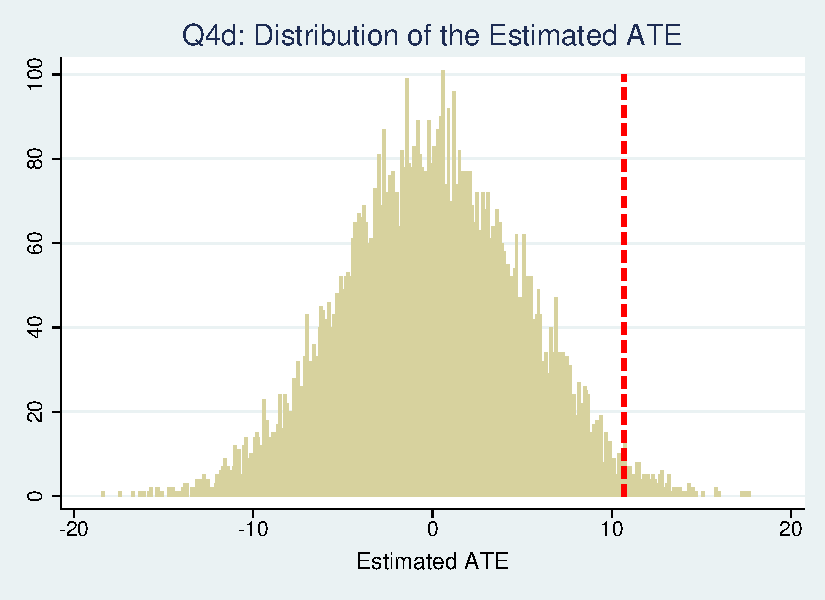
\includegraphics[width=4in,height=3.6in]{figure/exercise_4_4_d_graph} 

}



\end{knitrout}
We use a two-tailed test in order to evaluate the null hypothesis that the treatment has no effect for any subject.  We find a two-tailed $p$-value of 0.031, which leads us to reject the null hypothesis in favor of the alternative hypothesis that the treatment has some positive effect.

\item Using the estimator in part (c), use randomization inference to evaluate the sharp null hypothesis of no effect for any school. To obtain the sampling distribution under the sharp null hypothesis, simulate 100,000 random assignments, and for each simulated sample, estimate the ATE using a regression of $Y_i$ on $D_i$ and $X_i$.  Interpret the results.

\begin{knitrout}
\definecolor{shadecolor}{rgb}{0.969, 0.969, 0.969}\color{fgcolor}\begin{kframe}
    \begin{Verbatim}[commandchars=\\\{\}]
{\color{incolor}In [{\color{incolor}11}]:} \PY{k}{capture}\PY{k}{ program}\PY{k}{ drop} ate\PYZus{}cov
         \PY{k}{program} define ate\PYZus{}cov, rclass
         \PY{k}{	regress} y D x
         \PY{k}{    return}\PY{k}{ scalar} Ys=\PYZus{}b[D]
         end
         
         tsrtest D \PY{n+nf}{r}(Ys) using ate\PYZus{}cov\PY{l+m}{.}dta, overwrite: ate\PYZus{}cov
\end{Verbatim}

    \begin{Verbatim}[commandchars=\\\{\}]



Two-sample randomization test for theta=r(Ys) of ate\_cov by D

Combinations:   137846528820 = (40 choose 20)
Assuming null=0
Observed theta: 5.316

Minimum time needed for exact test (h:m:s):  164458:34:01
Reverting to Monte Carlo simulation.
Mode: simulation (10000 repetitions)

progress: |{\ldots}|

 p=0.00150 [one-tailed test of Ho:  theta(D==0)<=theta(D==1)]
 p=0.99840 [one-tailed test of Ho:  theta(D==0)>=theta(D==1)]
 p=0.00290 [two-tailed test of Ho:  theta(D==0)==theta(D==1)]

Saving log file to ate\_cov.dta{\ldots}done.

    \end{Verbatim}

    \begin{Verbatim}[commandchars=\\\{\}]
{\color{incolor}In [{\color{incolor}12}]:} \PY{c+c1}{//}\PY{c+c1}{a}\PY{c+c1}{t}\PY{c+c1}{e}\PY{c+c1}{\PYZus{}}\PY{c+c1}{c}\PY{c+c1}{o}\PY{c+c1}{v}
         \PY{k}{di} \PY{n+nf}{r}(obsvStat)
\end{Verbatim}

    \begin{Verbatim}[commandchars=\\\{\}]
5.3155362

    \end{Verbatim}

    \begin{Verbatim}[commandchars=\\\{\}]
{\color{incolor}In [{\color{incolor}13}]:} \PY{c+c1}{//}\PY{c+c1}{ }\PY{c+c1}{p}\PY{c+c1}{.}\PY{c+c1}{v}\PY{c+c1}{a}\PY{c+c1}{l}\PY{c+c1}{u}\PY{c+c1}{e}\PY{c+c1}{\PYZus{}}\PY{c+c1}{c}\PY{c+c1}{o}\PY{c+c1}{v}
         \PY{k}{di} \PY{n+nf}{r}(twotail)
\end{Verbatim}

    \begin{Verbatim}[commandchars=\\\{\}]
.00289971

    \end{Verbatim}
\end{kframe}
\end{knitrout}

We again use a two-tailed test in order to evaluate the null hypothesis that the treatment has no effect for any subject.  We find a two-tailed p-value of 0.003, which leads us to reject the null hypothesis in favor of the alternative hypothesis that the treatment has some effect.

\item Use the estimated ATE in part (a) to construct a full schedule of potential outcomes for all schools, assuming that every school has the same treatment effect. Using this simulated schedule of potential outcomes, construct a 95\% confidence interval for the sample average treatment effect in the following way. First, assign each subject to treatment or control, and estimate the ATE by a regression of $Y_i$ on $D_i$. Repeat this procedure until you have 100,000 estimates of the ATE.  Order the estimates from smallest to largest. The 2,501st estimate marks the 2.5th percentile, and the 97,500th estimate marks the 97.5th percentile. Interpret the results.

\begin{knitrout}
\definecolor{shadecolor}{rgb}{0.969, 0.969, 0.969}\color{fgcolor}\begin{kframe}
    \begin{Verbatim}[commandchars=\\\{\}]
{\color{incolor}In [{\color{incolor}14}]:} \PY{k}{cap}\PY{k}{ drop} Y0\PYZus{}sim Y1\PYZus{}sim Y\PYZus{}sim
         \PY{k}{qui}\PY{k}{ gen} Y0\PYZus{}sim = y
         \PY{k}{qui}\PY{k}{ gen} Y1\PYZus{}sim = y
         \PY{k}{qui}\PY{k}{ gen} Y\PYZus{}sim = .
         \PY{k}{qui}\PY{k}{ replace} Y0\PYZus{}sim = y \PY{o}{\PYZhy{}} \PY{n+nv+vg}{\PYZdl{}}\PY{n+nv+vg}{tau}\PY{k}{ if} D\PY{o}{==}\PY{l+m}{1}
         \PY{k}{qui}\PY{k}{ replace} Y1\PYZus{}sim = y \PY{o}{+} \PY{n+nv+vg}{\PYZdl{}}\PY{n+nv+vg}{tau}\PY{k}{ if} D\PY{o}{==}\PY{l+m}{0}
\end{Verbatim}

    \begin{Verbatim}[commandchars=\\\{\}]
{\color{incolor}In [{\color{incolor}15}]:} \PY{k}{capture}\PY{k}{ program}\PY{k}{ drop} ate\PYZus{}null
         \PY{k}{program} define ate\PYZus{}null, rclass
         \PY{k}{	replace} Y\PYZus{}sim = Y0\PYZus{}sim\PY{o}{*}(\PY{l+m}{1}\PY{o}{\PYZhy{}}D) \PY{o}{+} Y1\PYZus{}sim\PY{o}{*}(D) 
         \PY{k}{	regress} Y\PYZus{}sim D 
         \PY{k}{    return}\PY{k}{ scalar} Ys=\PYZus{}b[D]	
         end
         
         ritest D Ys = \PY{n+nf}{r}(Ys), reps(\PY{l+m}{10000})
         \PY{k}{ sav}(ate\PYZus{}null\PY{l+m}{.}dta,\PY{k}{ replace}) nodots: ate\PYZus{}null
\end{Verbatim}

    \begin{Verbatim}[commandchars=\\\{\}]


      Source |       SS           df       MS      Number of obs   =        40
-------------+----------------------------------   F(1, 38)        =      5.16
       Model |      1144.9         1      1144.9   Prob > F        =    0.0288
    Residual |      8427.5        38  221.776316   R-squared       =    0.1196
-------------+----------------------------------   Adj R-squared   =    0.0964
       Total |      9572.4        39  245.446154   Root MSE        =    14.892

------------------------------------------------------------------------------
       Y\_sim |      Coef.   Std. Err.      t    P>|t|     [95\% Conf. Interval]
-------------+----------------------------------------------------------------
           D |       10.7   4.709313     2.27   0.029     1.166494    20.23351
       \_cons |      26.85   3.329987     8.06   0.000     20.10879    33.59121
------------------------------------------------------------------------------

      command:  ate\_null
           Ys:  r(Ys)
  res. var(s):  D
   Resampling:  Permuting D
Clust. var(s):  \_\_00000J
     Clusters:  40
Strata var(s):  none
       Strata:  1

------------------------------------------------------------------------------
T            |     T(obs)       c       n   p=c/n   SE(p) [95\% Conf. Interval]
-------------+----------------------------------------------------------------
          Ys |       10.7    4996   10000  0.4996  0.0050  .4897515   .5094487
------------------------------------------------------------------------------
Note: Confidence interval is with respect to p=c/n.
Note: c = \#\{|T| >= |T(obs)|\}

    \end{Verbatim}

    \begin{Verbatim}[commandchars=\\\{\}]
{\color{incolor}In [{\color{incolor}16}]:} \PY{k}{preserve}
         \PY{c+c1}{//}\PY{c+c1}{ }\PY{c+c1}{C}\PY{c+c1}{I}\PY{c+c1}{ }\PY{c+c1}{a}\PY{c+c1}{n}\PY{c+c1}{d}\PY{c+c1}{ }\PY{c+c1}{H}\PY{c+c1}{i}\PY{c+c1}{s}\PY{c+c1}{t}
         \PY{k}{use} \PY{l+s}{\PYZdq{}}\PY{l+s}{a}\PY{l+s}{t}\PY{l+s}{e}\PY{l+s}{\PYZus{}}\PY{l+s}{n}\PY{l+s}{u}\PY{l+s}{l}\PY{l+s}{l}\PY{l+s}{.}\PY{l+s}{d}\PY{l+s}{t}\PY{l+s}{a}\PY{l+s}{\PYZdq{}},\PY{k}{ clear}
         
         \PY{k}{sort} Ys
         \PY{k}{global} ylower= \PY{n+nf}{round}(Ys[\PY{l+m}{251}], .\PY{l+m}{01})
         
         \PY{k}{global} yupper= \PY{n+nf}{round}(Ys[\PY{l+m}{9750}], .\PY{l+m}{01})
         \PY{k}{di} \PY{l+s}{\PYZdq{}}\PY{l+s}{9}\PY{l+s}{5}\PY{l+s}{\PYZpc{}}\PY{l+s}{C}\PY{l+s}{I}\PY{l+s}{:}\PY{l+s}{ }\PY{l+s}{(}\PY{n+nv+vg}{\PYZdl{}}\PY{n+nv+vg}{ylower}\PY{l+s}{,}\PY{l+s}{ }\PY{n+nv+vg}{\PYZdl{}}\PY{n+nv+vg}{yupper}\PY{l+s}{)}\PY{l+s}{\PYZdq{}} 
         
         \PY{k}{graph}\PY{k}{ twoway} (histogram Ys,frequency bin(\PY{l+m}{1000})) 
         (scatteri \PY{l+m}{0} \PY{n+nv+vg}{\PYZdl{}}\PY{n+nv+vg}{tau} \PY{l+m}{50} \PY{n+nv+vg}{\PYZdl{}}\PY{n+nv+vg}{tau}, \PY{n+nf}{c}(l) lc(red) lw(thick) lp(dash)\PY{k}{ m}(i)) 
         (scatteri \PY{l+m}{0} \PY{n+nv+vg}{\PYZdl{}}\PY{n+nv+vg}{ylower} \PY{l+m}{50} \PY{n+nv+vg}{\PYZdl{}}\PY{n+nv+vg}{ylower}, \PY{n+nf}{c}(l) lc(red) lw(thick) lp(dash)\PY{k}{ m}(i)) 
         (scatteri \PY{l+m}{0} \PY{n+nv+vg}{\PYZdl{}}\PY{n+nv+vg}{yupper} \PY{l+m}{50} \PY{n+nv+vg}{\PYZdl{}}\PY{n+nv+vg}{yupper}, \PY{n+nf}{c}(l) lc(red) lw(thick) lp(dash)\PY{k}{ m}(i)),
         legend(off) 
         b1title(\PY{l+s}{\PYZdq{}}\PY{l+s}{E}\PY{l+s}{s}\PY{l+s}{t}\PY{l+s}{i}\PY{l+s}{m}\PY{l+s}{a}\PY{l+s}{t}\PY{l+s}{e}\PY{l+s}{d}\PY{l+s}{ }\PY{l+s}{A}\PY{l+s}{T}\PY{l+s}{E}\PY{l+s}{\PYZdq{}}) 
         title(\PY{l+s}{\PYZdq{}}\PY{l+s}{D}\PY{l+s}{i}\PY{l+s}{s}\PY{l+s}{t}\PY{l+s}{r}\PY{l+s}{i}\PY{l+s}{b}\PY{l+s}{u}\PY{l+s}{t}\PY{l+s}{i}\PY{l+s}{o}\PY{l+s}{n}\PY{l+s}{ }\PY{l+s}{u}\PY{l+s}{n}\PY{l+s}{d}\PY{l+s}{e}\PY{l+s}{r}\PY{l+s}{ }\PY{l+s}{t}\PY{l+s}{h}\PY{l+s}{e}\PY{l+s}{ }\PY{l+s}{n}\PY{l+s}{u}\PY{l+s}{l}\PY{l+s}{l}\PY{l+s}{ }\PY{l+s}{A}\PY{l+s}{T}\PY{l+s}{E}\PY{l+s}{ }\PY{l+s}{=}\PY{l+s}{ }\PY{l+s}{1}\PY{l+s}{0}\PY{l+s}{.}\PY{l+s}{7}\PY{l+s}{\PYZdq{}}) \PY{c+cs}{///}
         xtitle(\PY{l+s}{\PYZdq{}}\PY{l+s}{\PYZdq{}})
         
         \PY{k}{graph} export .\PY{o}{/}exercise\PYZus{}4\PYZus{}4\PYZus{}f\PYZus{}graph\PY{l+m}{.}pdf
         
         \PY{k}{restore}
\end{Verbatim}

    \begin{Verbatim}[commandchars=\\\{\}]
95\%CI: (1.53, 19.83)
    \end{Verbatim}
\end{kframe}

{\centering 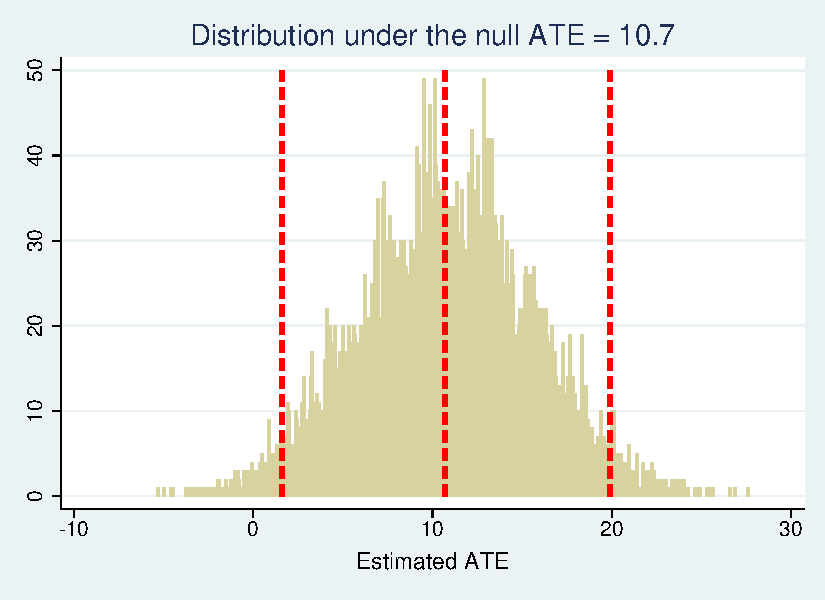
\includegraphics[width=4in,height=3.6in]{figure/exercise_4_4_f_graph} 

}


\end{knitrout}

The confidence interval stretches from [1.53, 19.83] implying that the ATE is positive but its location is subject to a great deal of statistical uncertainty.  Our best guess is 10.7, but the interval ranges from a small positive value to a truly massive effect.

\item Use the estimated ATE in part (c) to construct a full schedule of potential outcomes for all schools, assuming that every school has the same treatment effect.  Using this simulated schedule of potential outcomes, simulate the 95\% confidence interval for the sample average treatment effect estimated by a regression of $Y_i$ on $D_i$ and $X_i$.  Interpret the results.  Is this confidence interval narrower than one you generated in question (f)?  

\begin{knitrout}
\definecolor{shadecolor}{rgb}{0.969, 0.969, 0.969}\color{fgcolor}\begin{kframe}
    \begin{Verbatim}[commandchars=\\\{\}]
{\color{incolor}In [{\color{incolor}17}]:} \PY{k}{cap}\PY{k}{ drop} Y0\PYZus{}sim Y1\PYZus{}sim Y\PYZus{}sim
         \PY{k}{qui}\PY{k}{ gen} Y0\PYZus{}sim = y
         \PY{k}{qui}\PY{k}{ gen} Y1\PYZus{}sim = y
         \PY{k}{qui}\PY{k}{ gen} Y\PYZus{}sim = .
         \PY{k}{qui}\PY{k}{ replace} Y0\PYZus{}sim = y \PY{o}{\PYZhy{}} \PY{n+nv+vg}{\PYZdl{}}\PY{n+nv+vg}{tau\PYZus{}c}\PY{k}{ if} D\PY{o}{==}\PY{l+m}{1}
         \PY{k}{qui}\PY{k}{ replace} Y1\PYZus{}sim = y \PY{o}{+} \PY{n+nv+vg}{\PYZdl{}}\PY{n+nv+vg}{tau\PYZus{}c}\PY{k}{ if} D\PY{o}{==}\PY{l+m}{0}
\end{Verbatim}

    \begin{Verbatim}[commandchars=\\\{\}]
{\color{incolor}In [{\color{incolor}18}]:} \PY{k}{capture}\PY{k}{ program}\PY{k}{ drop} ate\PYZus{}null\PYZus{}cov
         \PY{k}{program} define ate\PYZus{}null\PYZus{}cov, rclass
         \PY{k}{	replace} Y\PYZus{}sim = Y0\PYZus{}sim\PY{o}{*}(\PY{l+m}{1}\PY{o}{\PYZhy{}}D) \PY{o}{+} Y1\PYZus{}sim\PY{o}{*}(D) 
         \PY{k}{	regress} Y\PYZus{}sim D x
         \PY{k}{    return}\PY{k}{ scalar} Ys\PYZus{}cov=\PYZus{}b[D]	
         end
         
         ritest D Ys\PYZus{}cov = \PY{n+nf}{r}(Ys\PYZus{}cov), reps(\PY{l+m}{10000})
         \PY{k}{ sav}(ate\PYZus{}null\PYZus{}cov\PY{l+m}{.}dta,\PY{k}{ replace}) nodots: \PY{c+cs}{///}
         ate\PYZus{}null\PYZus{}cov
\end{Verbatim}

    \begin{Verbatim}[commandchars=\\\{\}]

      Source |       SS           df       MS      Number of obs   =        40
-------------+----------------------------------   F(2, 37)        =    168.97
       Model |  8627.78597         2  4313.89298   Prob > F        =    0.0000
    Residual |  944.614033        37   25.530109   R-squared       =    0.9013
-------------+----------------------------------   Adj R-squared   =    0.8960
       Total |      9572.4        39  245.446154   Root MSE        =    5.0527

------------------------------------------------------------------------------
       Y\_sim |      Coef.   Std. Err.      t    P>|t|     [95\% Conf. Interval]
-------------+----------------------------------------------------------------
           D |   5.315536   1.628474     3.26   0.002     2.015935    8.615138
           x |   .9204212   .0537624    17.12   0.000     .8114883    1.029354
       \_cons |   1.216271   1.875729     0.65   0.521    -2.584317    5.016858
------------------------------------------------------------------------------

      command:  ate\_null\_cov
       Ys\_cov:  r(Ys\_cov)
  res. var(s):  D
   Resampling:  Permuting D
Clust. var(s):  \_\_00000M
     Clusters:  40
Strata var(s):  none
       Strata:  1

------------------------------------------------------------------------------
T            |     T(obs)       c       n   p=c/n   SE(p) [95\% Conf. Interval]
-------------+----------------------------------------------------------------
      Ys\_cov |   5.315536    4961   10000  0.4961  0.0050  .4862528   .5059495
------------------------------------------------------------------------------
Note: Confidence interval is with respect to p=c/n.
Note: c = \#\{|T| >= |T(obs)|\}

    \end{Verbatim}

    \begin{Verbatim}[commandchars=\\\{\}]
{\color{incolor}In [{\color{incolor}19}]:} \PY{k}{preserve}
        \PY{c+c1}{//}\PY{c+c1}{ }\PY{c+c1}{C}\PY{c+c1}{I}\PY{c+c1}{ }\PY{c+c1}{a}\PY{c+c1}{n}\PY{c+c1}{d}\PY{c+c1}{ }\PY{c+c1}{H}\PY{c+c1}{i}\PY{c+c1}{s}\PY{c+c1}{t}
        \PY{k}{use} \PY{l+s}{\PYZdq{}}\PY{l+s}{a}\PY{l+s}{t}\PY{l+s}{e}\PY{l+s}{\PYZus{}}\PY{l+s}{n}\PY{l+s}{u}\PY{l+s}{l}\PY{l+s}{l}\PY{l+s}{\PYZus{}}\PY{l+s}{c}\PY{l+s}{o}\PY{l+s}{v}\PY{l+s}{.}\PY{l+s}{d}\PY{l+s}{t}\PY{l+s}{a}\PY{l+s}{\PYZdq{}},\PY{k}{ clear}
        
        \PY{k}{sort} Ys\PYZus{}cov
        \PY{k}{global} yclower= \PY{n+nf}{round}(Ys\PYZus{}cov[\PY{l+m}{251}], .\PY{l+m}{001})
        \PY{k}{global} ycupper= \PY{n+nf}{round}(Ys\PYZus{}cov[\PY{l+m}{9750}], .\PY{l+m}{001})
        
        \PY{k}{di} \PY{l+s}{\PYZdq{}}\PY{l+s}{9}\PY{l+s}{5}\PY{l+s}{\PYZpc{}}\PY{l+s}{C}\PY{l+s}{I}\PY{l+s}{:}\PY{l+s}{ }\PY{l+s}{(}\PY{n+nv+vg}{\PYZdl{}}\PY{n+nv+vg}{yclower}\PY{l+s}{,}\PY{l+s}{ }\PY{n+nv+vg}{\PYZdl{}}\PY{n+nv+vg}{ycupper}\PY{l+s}{)}\PY{l+s}{\PYZdq{}} 
        
        \PY{k}{graph}\PY{k}{ twoway} (histogram Ys\PYZus{}cov,frequency bin(\PY{l+m}{1000})) 
        (scatteri \PY{l+m}{0} \PY{n+nv+vg}{\PYZdl{}}\PY{n+nv+vg}{tau\PYZus{}c} \PY{l+m}{40} \PY{n+nv+vg}{\PYZdl{}}\PY{n+nv+vg}{tau\PYZus{}c}, \PY{n+nf}{c}(l) lc(red) lw(thick) lp(dash)\PY{k}{ m}(i)) 
        (scatteri \PY{l+m}{0} \PY{n+nv+vg}{\PYZdl{}}\PY{n+nv+vg}{yclower} \PY{l+m}{40} \PY{n+nv+vg}{\PYZdl{}}\PY{n+nv+vg}{yclower}, \PY{n+nf}{c}(l) lc(red) lw(thick) lp(dash)\PY{k}{ m}(i)) 
        (scatteri \PY{l+m}{0} \PY{n+nv+vg}{\PYZdl{}}\PY{n+nv+vg}{ycupper} \PY{l+m}{40} \PY{n+nv+vg}{\PYZdl{}}\PY{n+nv+vg}{ycupper}, \PY{n+nf}{c}(l) lc(red) lw(thick) lp(dash)\PY{k}{ m}(i)), 
        legend(off) 
        b1title(\PY{l+s}{\PYZdq{}}\PY{l+s}{E}\PY{l+s}{s}\PY{l+s}{t}\PY{l+s}{i}\PY{l+s}{m}\PY{l+s}{a}\PY{l+s}{t}\PY{l+s}{e}\PY{l+s}{d}\PY{l+s}{ }\PY{l+s}{A}\PY{l+s}{T}\PY{l+s}{E}\PY{l+s}{ }\PY{l+s}{c}\PY{l+s}{o}\PY{l+s}{n}\PY{l+s}{t}\PY{l+s}{r}\PY{l+s}{o}\PY{l+s}{l}\PY{l+s}{l}\PY{l+s}{i}\PY{l+s}{n}\PY{l+s}{g}\PY{l+s}{ }\PY{l+s}{c}\PY{l+s}{o}\PY{l+s}{v}\PY{l+s}{a}\PY{l+s}{r}\PY{l+s}{i}\PY{l+s}{a}\PY{l+s}{n}\PY{l+s}{c}\PY{l+s}{e}\PY{l+s}{\PYZdq{}}) 
        title(\PY{l+s}{\PYZdq{}}\PY{l+s}{D}\PY{l+s}{i}\PY{l+s}{s}\PY{l+s}{t}\PY{l+s}{r}\PY{l+s}{i}\PY{l+s}{b}\PY{l+s}{u}\PY{l+s}{t}\PY{l+s}{i}\PY{l+s}{o}\PY{l+s}{n}\PY{l+s}{ }\PY{l+s}{u}\PY{l+s}{n}\PY{l+s}{d}\PY{l+s}{e}\PY{l+s}{r}\PY{l+s}{ }\PY{l+s}{t}\PY{l+s}{h}\PY{l+s}{e}\PY{l+s}{ }\PY{l+s}{n}\PY{l+s}{u}\PY{l+s}{l}\PY{l+s}{l}\PY{l+s}{ }\PY{l+s}{A}\PY{l+s}{T}\PY{l+s}{E}\PY{l+s}{ }\PY{l+s}{=}\PY{l+s}{ }\PY{l+s}{5}\PY{l+s}{.}\PY{l+s}{3}\PY{l+s}{\PYZdq{}}) 
        xtitle(\PY{l+s}{\PYZdq{}}\PY{l+s}{\PYZdq{}})
        
        \PY{k}{graph} export .\PY{o}{/}exercise\PYZus{}4\PYZus{}4\PYZus{}g\PYZus{}graph\PY{l+m}{.}pdf
        
        \PY{k}{restore}
\end{Verbatim}

    \begin{Verbatim}[commandchars=\\\{\}]
95\%CI: (2.213, 8.460)
    \end{Verbatim}
\end{kframe}
{\centering 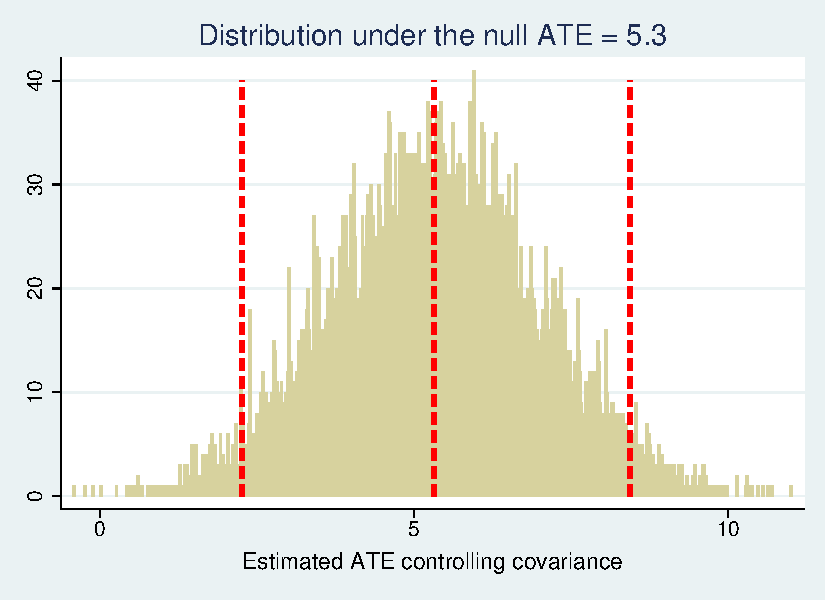
\includegraphics[width=4in,height=3.6in]{figure/exercise_4_4_g_graph} 

}

\end{knitrout}

The confidence interval now stretches from [2.22, 8.46].  Interestingly, this interval no longer contains the estimate obtained without controls for covariates.  Our best guess is now 5.3, and our 95\% interval is now roughly one-third as wide as before.

\end{enumerate}

\section*{Question 5}


Randomizations are said to be ``restricted'' when the set of all possible random allocations is narrowed to exclude allocations that have inadequate covariate balance.  Suppose, for example, that the assignment of treatments ($D_i$) in Table 4.1 was conducted subject to the restriction that a regression of $D_i$ on $X_i$ (the pretest) does not allow the researcher to reject the sharp null hypothesis of no effect of $X_i$ on $D_i$ at the 0.05 significance level) produces a $p$-value on that is greater than 0.05. In other words, had the researcher found that the assigned $D_i$ were significantly predicted by $X_i$, the random allocation would have been conducted again, until the $D_i$ met this criterion. [10pts]

\begin{enumerate}[a)]
\item Conduct a series of random assignments in order to calculate the weighting variable $w_i$; for units in the treatment group, this weight is defined as the inverse of the probability of being assigned to treatment, and for units in the control group, this weight is defined as the inverse of the probability of being assigned to control. See Table 4.2 for an example. Does $w_i$ appear to vary within the treatment group or within the control group?

\begin{knitrout}
\definecolor{shadecolor}{rgb}{0.969, 0.969, 0.969}\color{fgcolor}\begin{kframe}
    \begin{Verbatim}[commandchars=\\\{\}]
{\color{incolor}In [{\color{incolor}1}]:} \PY{k}{clear}
        \PY{k}{clear}\PY{k}{ matrix}
        \PY{k}{clear}\PY{k}{ mata}
        \PY{k}{set} matsize \PY{l+m}{11000} 
        \PY{k}{set} maxvar \PY{l+m}{32767}
        \PY{k}{set} seed \PY{l+m}{1234567}
        \PY{k}{set}\PY{k}{ more} off
\end{Verbatim}

    \begin{Verbatim}[commandchars=\\\{\}]
{\color{incolor}In [{\color{incolor}2}]:} 
\PY{c+c1}{//}\PY{c+c1}{ }\PY{c+c1}{l}\PY{c+c1}{o}\PY{c+c1}{o}\PY{c+c1}{p}\PY{c+c1}{ }\PY{c+c1}{t}\PY{c+c1}{o}\PY{c+c1}{ }\PY{c+c1}{s}\PY{c+c1}{i}\PY{c+c1}{m}\PY{c+c1}{u}\PY{c+c1}{l}\PY{c+c1}{t}\PY{c+c1}{e}\PY{c+c1}{ }\PY{c+c1}{r}\PY{c+c1}{a}\PY{c+c1}{n}\PY{c+c1}{d}\PY{c+c1}{o}\PY{c+c1}{m}\PY{c+c1}{ }\PY{c+c1}{a}\PY{c+c1}{s}\PY{c+c1}{s}\PY{c+c1}{i}\PY{c+c1}{g}\PY{c+c1}{n}\PY{c+c1}{m}\PY{c+c1}{e}\PY{c+c1}{n}\PY{c+c1}{t}\PY{c+c1}{ }\PY{c+c1}{a}\PY{c+c1}{n}\PY{c+c1}{d}\PY{c+c1}{ }\PY{c+c1}{s}\PY{c+c1}{a}\PY{c+c1}{v}\PY{c+c1}{e}\PY{c+c1}{ }\PY{c+c1}{t}\PY{c+c1}{o}\PY{c+c1}{ }\PY{c+c1}{a}\PY{c+c1}{ }\PY{c+c1}{m}\PY{c+c1}{a}\PY{c+c1}{t}\PY{c+c1}{r}\PY{c+c1}{i}\PY{c+c1}{x}\PY{c+c1}{ }       
        \PY{k}{cap}\PY{k}{ matrix}\PY{k}{ drop} z
        \PY{k}{matrix} z=\PY{n+nf}{J}(\PY{l+m}{40}, \PY{l+m}{10000}, .)
        
        \PY{k}{qui}\PY{k}{ forvalues} i = \PY{l+m}{1}\PY{o}{/}\PY{l+m}{10000} \PYZob{}
        \PY{c+c1}{//}\PY{c+c1}{c}\PY{c+c1}{r}\PY{c+c1}{e}\PY{c+c1}{a}\PY{c+c1}{t}\PY{c+c1}{e}\PY{c+c1}{ }\PY{c+c1}{a}\PY{c+c1}{n}\PY{c+c1}{d}\PY{c+c1}{ }\PY{c+c1}{s}\PY{c+c1}{a}\PY{c+c1}{v}\PY{c+c1}{e}\PY{c+c1}{ }\PY{c+c1}{5}\PY{c+c1}{0}\PY{c+c1}{ }\PY{c+c1}{p}\PY{c+c1}{e}\PY{c+c1}{r}\PY{c+c1}{m}\PY{c+c1}{u}\PY{c+c1}{t}\PY{c+c1}{a}\PY{c+c1}{t}\PY{c+c1}{i}\PY{c+c1}{o}\PY{c+c1}{n}\PY{c+c1}{s}\PY{c+c1}{ }\PY{c+c1}{o}\PY{c+c1}{f}\PY{c+c1}{ }\PY{c+c1}{t}\PY{c+c1}{r}\PY{c+c1}{e}\PY{c+c1}{a}\PY{c+c1}{t}\PY{c+c1}{m}\PY{c+c1}{e}\PY{c+c1}{n}\PY{c+c1}{t}
        	import delim 
       \PY{l+s}{\PYZdq{}}\PY{l+s}{.}\PY{l+s}{/}\PY{l+s}{d}\PY{l+s}{a}\PY{l+s}{t}\PY{l+s}{a}\PY{l+s}{/}\PY{l+s}{c}\PY{l+s}{h}\PY{l+s}{a}\PY{l+s}{p}\PY{l+s}{t}\PY{l+s}{e}\PY{l+s}{r}\PY{l+s}{0}\PY{l+s}{4}\PY{l+s}{/}\PY{l+s}{G}\PY{l+s}{e}\PY{l+s}{r}\PY{l+s}{b}\PY{l+s}{e}\PY{l+s}{r}\PY{l+s}{G}\PY{l+s}{r}\PY{l+s}{e}\PY{l+s}{e}\PY{l+s}{n}\PY{l+s}{B}\PY{l+s}{o}\PY{l+s}{o}\PY{l+s}{k}\PY{l+s}{\PYZus{}}\PY{l+s}{C}\PY{l+s}{h}\PY{l+s}{a}\PY{l+s}{p}\PY{l+s}{t}\PY{l+s}{e}\PY{l+s}{r}\PY{l+s}{4}\PY{l+s}{\PYZus{}}\PY{l+s}{E}\PY{l+s}{x}\PY{l+s}{e}\PY{l+s}{r}\PY{l+s}{c}\PY{l+s}{i}\PY{l+s}{s}\PY{l+s}{e}\PY{l+s}{s}\PY{l+s}{\PYZus{}}\PY{l+s}{4}\PY{l+s}{\PYZhy{}}\PY{l+s}{5}\PY{l+s}{.}\PY{l+s}{c}\PY{l+s}{s}\PY{l+s}{v}\PY{l+s}{\PYZdq{}}
        \PY{k}{	tempvar} teststat Z
        \PY{k}{	gen} \PY{n+nv}{`}\PY{n+nv}{Z}\PY{n+nv}{\PYZsq{}} = .
        \PY{k}{	gen} \PY{n+nv}{`}\PY{n+nv}{t}\PY{n+nv}{e}\PY{n+nv}{s}\PY{n+nv}{t}\PY{n+nv}{s}\PY{n+nv}{t}\PY{n+nv}{a}\PY{n+nv}{t}\PY{n+nv}{\PYZsq{}} = \PY{o}{\PYZhy{}}\PY{l+m}{1}
        \PY{k}{	while} \PY{n+nv}{`}\PY{n+nv}{t}\PY{n+nv}{e}\PY{n+nv}{s}\PY{n+nv}{t}\PY{n+nv}{s}\PY{n+nv}{t}\PY{n+nv}{a}\PY{n+nv}{t}\PY{n+nv}{\PYZsq{}} \PY{o}{\PYZlt{}} \PY{l+m}{0.05}\PYZob{}
        \PY{k}{		tempvar} rannum Zri t
        \PY{k}{	    gen} \PY{n+nv}{`}\PY{n+nv}{r}\PY{n+nv}{a}\PY{n+nv}{n}\PY{n+nv}{n}\PY{n+nv}{u}\PY{n+nv}{m}\PY{n+nv}{\PYZsq{}}=\PY{n+nf}{uniform}()
        \PY{k}{		egen} \PY{n+nv}{`}\PY{n+nv}{Z}\PY{n+nv}{r}\PY{n+nv}{i}\PY{n+nv}{\PYZsq{}} = cut(\PY{n+nv}{`}\PY{n+nv}{r}\PY{n+nv}{a}\PY{n+nv}{n}\PY{n+nv}{n}\PY{n+nv}{u}\PY{n+nv}{m}\PY{n+nv}{\PYZsq{}}), \PY{n+nf}{group}(\PY{l+m}{2})
        \PY{k}{		qui}\PY{k}{ reg} \PY{n+nv}{`}\PY{n+nv}{Z}\PY{n+nv}{r}\PY{n+nv}{i}\PY{n+nv}{\PYZsq{}} x
        \PY{k}{		gen} \PY{n+nv}{`}\PY{n+nv}{t}\PY{n+nv}{\PYZsq{}} = \PYZus{}b[x]\PY{o}{/}\PYZus{}se[x]		
        \PY{k}{		replace} \PY{n+nv}{`}\PY{n+nv}{t}\PY{n+nv}{e}\PY{n+nv}{s}\PY{n+nv}{t}\PY{n+nv}{s}\PY{n+nv}{t}\PY{n+nv}{a}\PY{n+nv}{t}\PY{n+nv}{\PYZsq{}} = \PY{l+m}{2}\PY{o}{*}\PY{n+nf}{ttail}(\PY{n+nf}{e}(df\PYZus{}r),\PY{n+nf}{abs}(\PY{n+nv}{`}\PY{n+nv}{t}\PY{n+nv}{\PYZsq{}}))	
        	\PYZcb{}
        \PY{k}{	replace} \PY{n+nv}{`}\PY{n+nv}{Z}\PY{n+nv}{\PYZsq{}} = \PY{n+nv}{`}\PY{n+nv}{Z}\PY{n+nv}{r}\PY{n+nv}{i}\PY{n+nv}{\PYZsq{}}
        \PY{k}{	forvalues} j = \PY{l+m}{1}\PY{o}{/}\PY{l+m}{40} \PYZob{}
        \PY{k}{	matrix} z[\PY{n+nv}{`}\PY{n+nv}{j}\PY{n+nv}{\PYZsq{}}, \PY{n+nv}{`}\PY{n+nv}{i}\PY{n+nv}{\PYZsq{}}] = \PY{n+nv}{`}\PY{n+nv}{Z}\PY{n+nv}{\PYZsq{}}[\PY{n+nv}{`}\PY{n+nv}{j}\PY{n+nv}{\PYZsq{}}]
        	\PYZcb{}
        \PY{k}{	drop} \PYZus{}all
        \PYZcb{}
\end{Verbatim}

    \begin{Verbatim}[commandchars=\\\{\}]
{\color{incolor}In [{\color{incolor}3}]:} \PY{k}{qui} import delim 
	\PY{l+s}{\PYZdq{}}\PY{l+s}{.}\PY{l+s}{/}\PY{l+s}{d}\PY{l+s}{a}\PY{l+s}{t}\PY{l+s}{a}\PY{l+s}{/}\PY{l+s}{c}\PY{l+s}{h}\PY{l+s}{a}\PY{l+s}{p}\PY{l+s}{t}\PY{l+s}{e}\PY{l+s}{r}\PY{l+s}{0}\PY{l+s}{4}\PY{l+s}{/}\PY{l+s}{G}\PY{l+s}{e}\PY{l+s}{r}\PY{l+s}{b}\PY{l+s}{e}\PY{l+s}{r}\PY{l+s}{G}\PY{l+s}{r}\PY{l+s}{e}\PY{l+s}{e}\PY{l+s}{n}\PY{l+s}{B}\PY{l+s}{o}\PY{l+s}{o}\PY{l+s}{k}\PY{l+s}{\PYZus{}}\PY{l+s}{C}\PY{l+s}{h}\PY{l+s}{a}\PY{l+s}{p}\PY{l+s}{t}\PY{l+s}{e}\PY{l+s}{r}\PY{l+s}{4}\PY{l+s}{\PYZus{}}\PY{l+s}{E}\PY{l+s}{x}\PY{l+s}{e}\PY{l+s}{r}\PY{l+s}{c}\PY{l+s}{i}\PY{l+s}{s}\PY{l+s}{e}\PY{l+s}{s}\PY{l+s}{\PYZus{}}\PY{l+s}{4}\PY{l+s}{\PYZhy{}}\PY{l+s}{5}\PY{l+s}{.}\PY{l+s}{c}\PY{l+s}{s}\PY{l+s}{v}\PY{l+s}{\PYZdq{}},\PY{k}{ clear}
        \PY{k}{rename}\PY{k}{ d} D
        \PY{k}{rename} y Y
        \PY{k}{matrix} rowm = z \PY{o}{*} \PY{n+nf}{J}(\PY{n+nf}{colsof}(z), \PY{l+m}{1}, \PY{l+m}{1}\PY{o}{/}\PY{n+nf}{colsof}(z))
        \PY{k}{matrix} colnames rowm=probs
        \PY{k}{svmat} double rowm, names(col)       
        \PY{k}{qui}\PY{k}{ gen} weights = (\PY{l+m}{1}\PY{o}{/}probs)\PY{o}{*}D \PY{o}{+}(\PY{l+m}{1}\PY{o}{/}(\PY{l+m}{1}\PY{o}{\PYZhy{}}probs))\PY{o}{*}(\PY{l+m}{1}\PY{o}{\PYZhy{}}D)        
        \PY{k}{tabstat} weights,\PY{k}{ by}(D) stat(v)
\end{Verbatim}

    \begin{Verbatim}[commandchars=\\\{\}]
Summary for variables: weights
     by categories of: D (D)

       D |  variance
---------+----------
       0 |  .0004185
       1 |   .000625
---------+----------
   Total |  .0005084
--------------------

    \end{Verbatim}
\end{kframe}
\end{knitrout}

The variance of the weights is \ensuremath{4\times 10^{-4}} in the treatment condition and \ensuremath{6\times 10^{-4}} in the control condition. Indeed, units do have different probabilities of assignments as a result of the restriction scheme, but the differences are small.

\item Use randomization inference to test the sharp null hypothesis that $D_i$ has no effect on $Y_i$ by regressing $Y_i$ on $D_i$ and comparing the estimate to the sampling distribution under the null hypothesis. Make sure that your sampling distribution includes only random allocations that satisfy the restriction mentioned above. Be sure to weight units by inverse probability weights as produced by the random allocation procedure. Estimate the ATE, calculate the $p$-value, and interpret the results.

\begin{knitrout}
\definecolor{shadecolor}{rgb}{0.969, 0.969, 0.969}\color{fgcolor}\begin{kframe}
    \begin{Verbatim}[commandchars=\\\{\}]
{\color{incolor}In [{\color{incolor}4}]:} \PY{k}{qui}\PY{k}{ reg} Y D [pw=weights]
        \PY{k}{global} ate\PYZus{}restricted\PYZus{}RA = \PYZus{}b[D]
        
        \PY{k}{di} \PY{l+s}{\PYZdq{}}\PY{l+s}{A}\PY{l+s}{T}\PY{l+s}{E}\PY{l+s}{ }\PY{l+s}{(}\PY{l+s}{R}\PY{l+s}{e}\PY{l+s}{s}\PY{l+s}{t}\PY{l+s}{r}\PY{l+s}{i}\PY{l+s}{c}\PY{l+s}{t}\PY{l+s}{e}\PY{l+s}{d}\PY{l+s}{ }\PY{l+s}{A}\PY{l+s}{s}\PY{l+s}{s}\PY{l+s}{i}\PY{l+s}{g}\PY{l+s}{n}\PY{l+s}{m}\PY{l+s}{e}\PY{l+s}{n}\PY{l+s}{t}\PY{l+s}{)}\PY{l+s}{=}\PY{l+s}{ }\PY{l+s}{\PYZdq{}} \PY{n+nv+vg}{\PYZdl{}}\PY{n+nv+vg}{ate\PYZus{}restricted\PYZus{}RA}
\end{Verbatim}

    \begin{Verbatim}[commandchars=\\\{\}]
ATE (Restricted Assignment)= 10.712532
    \end{Verbatim}

    \begin{Verbatim}[commandchars=\\\{\}]
{\color{incolor}In [{\color{incolor}5}]:} \PY{k}{svmat} z
        
        \PY{k}{cap}\PY{k}{ matrix}\PY{k}{ drop} y\PYZus{}dis
        \PY{k}{matrix} y\PYZus{}dis=\PY{n+nf}{J}(\PY{l+m}{10000}, \PY{l+m}{1}, .)
        
        \PY{k}{forvalues} i = \PY{l+m}{1}\PY{o}{/}\PY{l+m}{10000} \PYZob{}
        \PY{k}{	tempvar} weight\PY{n+nv}{`}\PY{n+nv}{i}\PY{n+nv}{\PYZsq{}}
        \PY{k}{	gen} \PY{n+nv}{`}\PY{n+nv}{w}\PY{n+nv}{e}\PY{n+nv}{i}\PY{n+nv}{g}\PY{n+nv}{h}\PY{n+nv}{t}\PY{n+nv}{`}\PY{n+nv}{i}\PY{n+nv}{\PYZsq{}}\PY{n+nv}{\PYZsq{}} = (\PY{l+m}{1}\PY{o}{/}probs)\PY{o}{*}z\PY{n+nv}{`}\PY{n+nv}{i}\PY{n+nv}{\PYZsq{}} \PY{o}{+}(\PY{l+m}{1}\PY{o}{/}(\PY{l+m}{1}\PY{o}{\PYZhy{}}probs))\PY{o}{*}(\PY{l+m}{1}\PY{o}{\PYZhy{}}z\PY{n+nv}{`}\PY{n+nv}{i}\PY{n+nv}{\PYZsq{}})
        \PY{k}{	qui}\PY{k}{ reg} Y z\PY{n+nv}{`}\PY{n+nv}{i}\PY{n+nv}{\PYZsq{}} [pw=\PY{n+nv}{`}\PY{n+nv}{w}\PY{n+nv}{e}\PY{n+nv}{i}\PY{n+nv}{g}\PY{n+nv}{h}\PY{n+nv}{t}\PY{n+nv}{`}\PY{n+nv}{i}\PY{n+nv}{\PYZsq{}}\PY{n+nv}{\PYZsq{}}]
        \PY{k}{	matrix} y\PYZus{}dis[\PY{n+nv}{`}\PY{n+nv}{i}\PY{n+nv}{\PYZsq{}}, \PY{l+m}{1}] = \PYZus{}b[z\PY{n+nv}{`}\PY{n+nv}{i}\PY{n+nv}{\PYZsq{}}]
        
        \PYZcb{}
\end{Verbatim}

    \begin{Verbatim}[commandchars=\\\{\}]
{\color{incolor}In [{\color{incolor}6}]:} \PY{k}{preserve}
         \PY{k}{svmat} y\PYZus{}dis      
         \PY{c+c1}{//}\PY{c+c1}{ }\PY{c+c1}{p}\PY{c+c1}{ }\PY{c+c1}{v}\PY{c+c1}{a}\PY{c+c1}{l}\PY{c+c1}{u}\PY{c+c1}{e}
         \PY{k}{count}\PY{k}{ if} \PY{n+nf}{abs}(y\PYZus{}dis1) \PY{o}{\PYZgt{}} \PY{n+nf}{abs}(\PY{n+nv+vg}{\PYZdl{}}\PY{n+nv+vg}{ate\PYZus{}restricted\PYZus{}RA})
         \PY{k}{di} \PY{n+nf}{r}(N)\PY{o}{/}\PYZus{}N
         \PY{k}{restore}
\end{Verbatim}

    \begin{Verbatim}[commandchars=\\\{\}]
  56

.0056
    \end{Verbatim}
\end{kframe}
\end{knitrout}


The IPW estimate of the ATE is 10.71, which is close to the unweighted estimate above.  Using a two-tailed test in order to evaluate the null hypothesis that the treatment has no effect for any subject, we find a p-value of 0.0056, which leads us to reject the null hypothesis in favor of the alternative hypothesis that the treatment has some effect. 

\item Use randomization inference to test the sharp null hypothesis that $D_i$ has no effect on $Y_i$ by regressing $Y_i$ on $D_i$ and $X_i$ and comparing the estimate to the sampling distribution under the null hypothesis.  Estimate the ATE, calculate the $p$-value, and interpret the results. 


\begin{knitrout}
\definecolor{shadecolor}{rgb}{0.969, 0.969, 0.969}\color{fgcolor}\begin{kframe}
    \begin{Verbatim}[commandchars=\\\{\}]
{\color{incolor}In [{\color{incolor}7}]:} \PY{k}{qui}\PY{k}{ reg} Y x D [pw=weights]
         \PY{k}{global} ate\PYZus{}cov\PYZus{}restricted\PYZus{}RA = \PYZus{}b[D]
         \PY{k}{di} \PY{l+s}{\PYZdq{}}\PY{l+s}{A}\PY{l+s}{T}\PY{l+s}{E}\PY{l+s}{ }\PY{l+s}{C}\PY{l+s}{o}\PY{l+s}{n}\PY{l+s}{t}\PY{l+s}{r}\PY{l+s}{o}\PY{l+s}{l}\PY{l+s}{l}\PY{l+s}{i}\PY{l+s}{n}\PY{l+s}{g}\PY{l+s}{ }\PY{l+s}{C}\PY{l+s}{o}\PY{l+s}{v}\PY{l+s}{a}\PY{l+s}{r}\PY{l+s}{i}\PY{l+s}{a}\PY{l+s}{n}\PY{l+s}{c}\PY{l+s}{e}\PY{l+s}{ }\PY{l+s}{(}\PY{l+s}{R}\PY{l+s}{e}\PY{l+s}{s}\PY{l+s}{t}\PY{l+s}{r}\PY{l+s}{i}\PY{l+s}{c}\PY{l+s}{t}\PY{l+s}{e}\PY{l+s}{d}\PY{l+s}{ }\PY{l+s}{A}\PY{l+s}{s}\PY{l+s}{s}\PY{l+s}{i}\PY{l+s}{g}\PY{l+s}{n}\PY{l+s}{m}\PY{l+s}{e}\PY{l+s}{n}\PY{l+s}{t}\PY{l+s}{)}\PY{l+s}{=}\PY{l+s}{ }\PY{l+s}{\PYZdq{}} 
        		 \PY{n+nv+vg}{\PYZdl{}}\PY{n+nv+vg}{ate\PYZus{}cov\PYZus{}restricted\PYZus{}RA}
\end{Verbatim}

    \begin{Verbatim}[commandchars=\\\{\}]
ATE Controlling Covariance (Restricted Assignment)= 5.3186105
    \end{Verbatim}

    \begin{Verbatim}[commandchars=\\\{\}]
{\color{incolor}In [{\color{incolor}8}]:} \PY{k}{cap}\PY{k}{ matrix}\PY{k}{ drop} cov\PYZus{}dis
         \PY{k}{matrix} cov\PYZus{}dis=\PY{n+nf}{J}(\PY{l+m}{10000}, \PY{l+m}{1}, .)        
         \PY{k}{forvalues} i = \PY{l+m}{1}\PY{o}{/}\PY{l+m}{10000}\PYZob{}
         \PY{k}{		tempvar} weight\PY{n+nv}{`}\PY{n+nv}{i}\PY{n+nv}{\PYZsq{}}
         \PY{k}{		gen} \PY{n+nv}{`}\PY{n+nv}{w}\PY{n+nv}{e}\PY{n+nv}{i}\PY{n+nv}{g}\PY{n+nv}{h}\PY{n+nv}{t}\PY{n+nv}{`}\PY{n+nv}{i}\PY{n+nv}{\PYZsq{}}\PY{n+nv}{\PYZsq{}} = (\PY{l+m}{1}\PY{o}{/}probs)\PY{o}{*}z\PY{n+nv}{`}\PY{n+nv}{i}\PY{n+nv}{\PYZsq{}} \PY{o}{+}(\PY{l+m}{1}\PY{o}{/}(\PY{l+m}{1}\PY{o}{\PYZhy{}}probs))\PY{o}{*}(\PY{l+m}{1}\PY{o}{\PYZhy{}}z\PY{n+nv}{`}\PY{n+nv}{i}\PY{n+nv}{\PYZsq{}})
         \PY{k}{		qui}\PY{k}{ reg} Y x z\PY{n+nv}{`}\PY{n+nv}{i}\PY{n+nv}{\PYZsq{}} [pw=\PY{n+nv}{`}\PY{n+nv}{w}\PY{n+nv}{e}\PY{n+nv}{i}\PY{n+nv}{g}\PY{n+nv}{h}\PY{n+nv}{t}\PY{n+nv}{`}\PY{n+nv}{i}\PY{n+nv}{\PYZsq{}}\PY{n+nv}{\PYZsq{}}]		
         \PY{k}{		matrix} cov\PYZus{}dis[\PY{n+nv}{`}\PY{n+nv}{i}\PY{n+nv}{\PYZsq{}}, \PY{l+m}{1}] = \PYZus{}b[z\PY{n+nv}{`}\PY{n+nv}{i}\PY{n+nv}{\PYZsq{}}]
         
         \PYZcb{}
\end{Verbatim}

    \begin{Verbatim}[commandchars=\\\{\}]
{\color{incolor}In [{\color{incolor}9}]:} \PY{k}{preserve}
         \PY{k}{svmat} cov\PYZus{}dis
         
         \PY{c+c1}{//}\PY{c+c1}{ }\PY{c+c1}{p}\PY{c+c1}{.}\PY{c+c1}{v}\PY{c+c1}{a}\PY{c+c1}{l}\PY{c+c1}{u}\PY{c+c1}{e}\PY{c+c1}{ }\PY{c+c1}{c}\PY{c+c1}{o}\PY{c+c1}{n}\PY{c+c1}{t}\PY{c+c1}{r}\PY{c+c1}{o}\PY{c+c1}{l}\PY{c+c1}{l}\PY{c+c1}{i}\PY{c+c1}{n}\PY{c+c1}{g}\PY{c+c1}{ }\PY{c+c1}{c}\PY{c+c1}{o}\PY{c+c1}{v}\PY{c+c1}{a}\PY{c+c1}{r}\PY{c+c1}{i}\PY{c+c1}{a}\PY{c+c1}{n}\PY{c+c1}{c}\PY{c+c1}{e}
         \PY{k}{count}\PY{k}{ if} \PY{n+nf}{abs}(cov\PYZus{}dis1) \PY{o}{\PYZgt{}} \PY{n+nf}{abs}(\PY{n+nv+vg}{\PYZdl{}}\PY{n+nv+vg}{ate\PYZus{}cov\PYZus{}restricted\PYZus{}RA})
         \PY{k}{di} \PY{n+nf}{r}(N)\PY{o}{/}\PYZus{}N
         \PY{k}{restore}
\end{Verbatim}

    \begin{Verbatim}[commandchars=\\\{\}]
  28

.0028
    \end{Verbatim}

\end{kframe}
\end{knitrout}

The IPW estimate of the ATE is 5.32, which is close to the unweighted estimate above. We again use a two-tailed test in order to evaluate the null hypothesis that the treatment has no effect for any subject. We find a $p$-value of 0.0028, which leads us to reject the null hypothesis in favor of the alternative hypothesis that the treatment has some effect.

\item Compare the sampling distributions under the null hypothesis in parts (a) and (b) to the sampling distributions obtained in exercises 4(d) and 4(e), which assumed that the randomization was unrestricted.  

\begin{knitrout}
\definecolor{shadecolor}{rgb}{0.969, 0.969, 0.969}\color{fgcolor}\begin{kframe}

    \begin{Verbatim}[commandchars=\\\{\}]
{\color{incolor}In [{\color{incolor}10}]:} \PY{c+cm}{/*}\PY{c+cm}{\PYZhy{}}\PY{c+cm}{\PYZhy{}}\PY{c+cm}{\PYZhy{}}\PY{c+cm}{\PYZhy{}}\PY{c+cm}{\PYZhy{}}\PY{c+cm}{\PYZhy{}}\PY{c+cm}{\PYZhy{}}\PY{c+cm}{\PYZhy{}}\PY{c+cm}{\PYZhy{}}\PY{c+cm}{\PYZhy{}}\PY{c+cm}{\PYZhy{}}\PY{c+cm}{\PYZhy{}}\PY{c+cm}{\PYZhy{}}\PY{c+cm}{\PYZhy{}}\PY{c+cm}{\PYZhy{}}\PY{c+cm}{\PYZhy{}}\PY{c+cm}{\PYZhy{}}\PY{c+cm}{\PYZhy{}}\PY{c+cm}{\PYZhy{}}\PY{c+cm}{\PYZhy{}}\PY{c+cm}{\PYZhy{}}\PY{c+cm}{\PYZhy{}}\PY{c+cm}{s}\PY{c+cm}{e}\PY{c+cm}{\PYZus{}}\PY{c+cm}{c}\PY{c+cm}{o}\PY{c+cm}{m}\PY{c+cm}{p}\PY{c+cm}{l}\PY{c+cm}{e}\PY{c+cm}{t}\PY{c+cm}{e}\PY{c+cm}{\PYZus{}}\PY{c+cm}{R}\PY{c+cm}{A}
         
         \PY{c+c1}{//}\PY{c+c1}{ }\PY{c+c1}{c}\PY{c+c1}{a}\PY{c+c1}{l}\PY{c+c1}{c}\PY{c+c1}{u}\PY{c+c1}{l}\PY{c+c1}{a}\PY{c+c1}{t}\PY{c+c1}{e}\PY{c+c1}{ }\PY{c+c1}{a}\PY{c+c1}{t}\PY{c+c1}{e}\PY{c+c1}{\PYZus{}}\PY{c+c1}{c}\PY{c+c1}{o}\PY{c+c1}{m}\PY{c+c1}{p}\PY{c+c1}{l}\PY{c+c1}{e}\PY{c+c1}{t}\PY{c+c1}{e}\PY{c+c1}{\PYZus{}}\PY{c+c1}{R}\PY{c+c1}{A}
         \PY{k}{qui}\PY{k}{ reg} Y D
         \PY{k}{global} ate\PYZus{}complete\PYZus{}RA = \PYZus{}b[D]
         \PY{k}{di} \PY{l+s}{\PYZdq{}}\PY{l+s}{A}\PY{l+s}{T}\PY{l+s}{E}\PY{l+s}{ }\PY{l+s}{u}\PY{l+s}{n}\PY{l+s}{d}\PY{l+s}{e}\PY{l+s}{r}\PY{l+s}{ }\PY{l+s}{C}\PY{l+s}{o}\PY{l+s}{m}\PY{l+s}{p}\PY{l+s}{l}\PY{l+s}{e}\PY{l+s}{t}\PY{l+s}{e}\PY{l+s}{ }\PY{l+s}{A}\PY{l+s}{s}\PY{l+s}{s}\PY{l+s}{i}\PY{l+s}{g}\PY{l+s}{n}\PY{l+s}{m}\PY{l+s}{e}\PY{l+s}{n}\PY{l+s}{t}\PY{l+s}{ }\PY{l+s}{=}\PY{l+s}{ }\PY{l+s}{\PYZdq{}} \PY{n+nv+vg}{\PYZdl{}}\PY{n+nv+vg}{ate\PYZus{}complete\PYZus{}RA}
\end{Verbatim}

    \begin{Verbatim}[commandchars=\\\{\}]
ATE under Complete Assignment = 10.7
    \end{Verbatim}

    \begin{Verbatim}[commandchars=\\\{\}]
{\color{incolor}In [{\color{incolor}11}]:} \PY{c+c1}{//}\PY{c+c1}{ }\PY{c+c1}{R}\PY{c+c1}{I}\PY{c+c1}{ }\PY{c+c1}{u}\PY{c+c1}{n}\PY{c+c1}{d}\PY{c+c1}{e}\PY{c+c1}{r}\PY{c+c1}{ }\PY{c+c1}{t}\PY{c+c1}{h}\PY{c+c1}{e}\PY{c+c1}{ }\PY{c+c1}{n}\PY{c+c1}{u}\PY{c+c1}{l}\PY{c+c1}{l}\PY{c+c1}{ }\PY{c+c1}{a}\PY{c+c1}{t}\PY{c+c1}{e}\PY{c+c1}{=}\PY{c+c1}{a}\PY{c+c1}{t}\PY{c+c1}{e}\PY{c+c1}{\PYZus{}}\PY{c+c1}{c}\PY{c+c1}{o}\PY{c+c1}{m}\PY{c+c1}{p}\PY{c+c1}{l}\PY{c+c1}{e}\PY{c+c1}{t}\PY{c+c1}{e}\PY{c+c1}{\PYZus{}}\PY{c+c1}{R}\PY{c+c1}{A}
         \PY{k}{cap}\PY{k}{ drop} Y0\PYZus{}sim Y1\PYZus{}sim Y\PYZus{}sim
         \PY{k}{qui}\PY{k}{ gen} Y0\PYZus{}sim = Y
         \PY{k}{qui}\PY{k}{ gen} Y1\PYZus{}sim = Y
         \PY{k}{qui}\PY{k}{ gen} Y\PYZus{}sim = .
         \PY{k}{qui}\PY{k}{ replace} Y0\PYZus{}sim = Y \PY{o}{\PYZhy{}} \PY{n+nv+vg}{\PYZdl{}}\PY{n+nv+vg}{ate\PYZus{}complete\PYZus{}RA}\PY{k}{ if} D\PY{o}{==}\PY{l+m}{1}
         \PY{k}{qui}\PY{k}{ replace} Y1\PYZus{}sim = Y \PY{o}{+} \PY{n+nv+vg}{\PYZdl{}}\PY{n+nv+vg}{ate\PYZus{}complete\PYZus{}RA}\PY{k}{ if} D\PY{o}{==}\PY{l+m}{0}
\end{Verbatim}

    \begin{Verbatim}[commandchars=\\\{\}]
{\color{incolor}In [{\color{incolor}12}]:} \PY{k}{capture}\PY{k}{ program}\PY{k}{ drop} ate\PYZus{}complete\PYZus{}RA\PYZus{}ri
         \PY{k}{program} define ate\PYZus{}complete\PYZus{}RA\PYZus{}ri, rclass
         \PY{k}{	replace} Y\PYZus{}sim = Y0\PYZus{}sim\PY{o}{*}(\PY{l+m}{1}\PY{o}{\PYZhy{}}D) \PY{o}{+} Y1\PYZus{}sim\PY{o}{*}(D) 
         \PY{k}{	regress} Y\PYZus{}sim D 
         \PY{k}{    return}\PY{k}{ scalar} Ys\PYZus{}complete\PYZus{}RA=\PYZus{}b[D]	
         end
         
         tsrtest D \PY{n+nf}{r}(Ys\PYZus{}complete\PYZus{}RA) using distout\PYZus{}complete\PYZus{}RA\PY{l+m}{.}dta, \PY{c+cs}{///}
         overwrite: ate\PYZus{}complete\PYZus{}RA\PYZus{}ri
\end{Verbatim}

    \begin{Verbatim}[commandchars=\\\{\}]
Two-sample randomization test for 
theta=r(Ys\_complete\_RA) of ate\_complete\_RA\_ri by D

Combinations:   137846528820 = (40 choose 20)
Assuming null=0
Observed theta: 10.7

Minimum time needed for exact test (h:m:s):  392479:42:00
Reverting to Monte Carlo simulation.
Mode: simulation (10000 repetitions)

progress: |{\ldots}|

 p=0.48995 [one-tailed test of Ho:  theta(D==0)<=theta(D==1)]
 p=0.50995 [one-tailed test of Ho:  theta(D==0)>=theta(D==1)]
 p=0.48995 [two-tailed test of Ho:  theta(D==0)==theta(D==1)]

Saving log file to distout\_complete\_RA.dta{\ldots}done.

    \end{Verbatim}

    \begin{Verbatim}[commandchars=\\\{\}]
{\color{incolor}In [{\color{incolor}13}]:} \PY{c+c1}{//}\PY{c+c1}{ }\PY{c+c1}{c}\PY{c+c1}{a}\PY{c+c1}{l}\PY{c+c1}{c}\PY{c+c1}{u}\PY{c+c1}{l}\PY{c+c1}{a}\PY{c+c1}{t}\PY{c+c1}{e}\PY{c+c1}{ }\PY{c+c1}{s}\PY{c+c1}{e}\PY{c+c1}{\PYZus{}}\PY{c+c1}{c}\PY{c+c1}{o}\PY{c+c1}{m}\PY{c+c1}{p}\PY{c+c1}{l}\PY{c+c1}{e}\PY{c+c1}{t}\PY{c+c1}{e}\PY{c+c1}{\PYZus{}}\PY{c+c1}{R}\PY{c+c1}{A}
         \PY{k}{preserve}
         \PY{k}{use} \PY{l+s}{\PYZdq{}}\PY{l+s}{d}\PY{l+s}{i}\PY{l+s}{s}\PY{l+s}{t}\PY{l+s}{o}\PY{l+s}{u}\PY{l+s}{t}\PY{l+s}{\PYZus{}}\PY{l+s}{c}\PY{l+s}{o}\PY{l+s}{m}\PY{l+s}{p}\PY{l+s}{l}\PY{l+s}{e}\PY{l+s}{t}\PY{l+s}{e}\PY{l+s}{\PYZus{}}\PY{l+s}{R}\PY{l+s}{A}\PY{l+s}{.}\PY{l+s}{d}\PY{l+s}{t}\PY{l+s}{a}\PY{l+s}{\PYZdq{}},\PY{k}{ clear}
         \PY{k}{qui}\PY{k}{ drop}\PY{k}{ if} \PYZus{}n\PY{o}{==}\PY{l+m}{1}
         \PY{k}{tabstat} theta, stat(sd)
         \PY{k}{restore}
\end{Verbatim}

    \begin{Verbatim}[commandchars=\\\{\}]
    variable |        sd
-------------+----------
       theta |  4.673591
------------------------


    \end{Verbatim}

    \begin{Verbatim}[commandchars=\\\{\}]
{\color{incolor}In [{\color{incolor}14}]:} \PY{c+cm}{/*}\PY{c+cm}{\PYZhy{}}\PY{c+cm}{\PYZhy{}}\PY{c+cm}{\PYZhy{}}\PY{c+cm}{\PYZhy{}}\PY{c+cm}{\PYZhy{}}\PY{c+cm}{\PYZhy{}}\PY{c+cm}{\PYZhy{}}\PY{c+cm}{\PYZhy{}}\PY{c+cm}{\PYZhy{}}\PY{c+cm}{\PYZhy{}}\PY{c+cm}{\PYZhy{}}\PY{c+cm}{\PYZhy{}}\PY{c+cm}{\PYZhy{}}\PY{c+cm}{\PYZhy{}}\PY{c+cm}{\PYZhy{}}\PY{c+cm}{\PYZhy{}}\PY{c+cm}{\PYZhy{}}\PY{c+cm}{\PYZhy{}}\PY{c+cm}{\PYZhy{}}\PY{c+cm}{\PYZhy{}}\PY{c+cm}{s}\PY{c+cm}{e}\PY{c+cm}{\PYZus{}}\PY{c+cm}{c}\PY{c+cm}{o}\PY{c+cm}{v}\PY{c+cm}{\PYZus{}}\PY{c+cm}{c}\PY{c+cm}{o}\PY{c+cm}{m}\PY{c+cm}{p}\PY{c+cm}{l}\PY{c+cm}{e}\PY{c+cm}{t}\PY{c+cm}{e}\PY{c+cm}{\PYZus{}}\PY{c+cm}{R}\PY{c+cm}{A}
         
         \PY{c+c1}{//}\PY{c+c1}{ }\PY{c+c1}{c}\PY{c+c1}{a}\PY{c+c1}{l}\PY{c+c1}{c}\PY{c+c1}{u}\PY{c+c1}{l}\PY{c+c1}{a}\PY{c+c1}{t}\PY{c+c1}{e}\PY{c+c1}{ }\PY{c+c1}{a}\PY{c+c1}{t}\PY{c+c1}{e}\PY{c+c1}{\PYZus{}}\PY{c+c1}{c}\PY{c+c1}{o}\PY{c+c1}{v}\PY{c+c1}{\PYZus{}}\PY{c+c1}{c}\PY{c+c1}{o}\PY{c+c1}{m}\PY{c+c1}{p}\PY{c+c1}{l}\PY{c+c1}{e}\PY{c+c1}{t}\PY{c+c1}{e}\PY{c+c1}{\PYZus{}}\PY{c+c1}{R}\PY{c+c1}{A}
         \PY{k}{qui}\PY{k}{ reg} Y D x
         \PY{k}{global} ate\PYZus{}cov\PYZus{}complete\PYZus{}RA = \PYZus{}b[D]
         \PY{k}{di} \PY{l+s}{\PYZdq{}}\PY{l+s}{A}\PY{l+s}{T}\PY{l+s}{E}\PY{l+s}{ }\PY{l+s}{C}\PY{l+s}{o}\PY{l+s}{n}\PY{l+s}{t}\PY{l+s}{r}\PY{l+s}{o}\PY{l+s}{l}\PY{l+s}{l}\PY{l+s}{i}\PY{l+s}{n}\PY{l+s}{g}\PY{l+s}{ }\PY{l+s}{C}\PY{l+s}{o}\PY{l+s}{v}\PY{l+s}{a}\PY{l+s}{r}\PY{l+s}{i}\PY{l+s}{a}\PY{l+s}{n}\PY{l+s}{c}\PY{l+s}{e}\PY{l+s}{ }\PY{l+s}{u}\PY{l+s}{n}\PY{l+s}{d}\PY{l+s}{e}\PY{l+s}{r}\PY{l+s}{ }\PY{l+s}{C}\PY{l+s}{o}\PY{l+s}{m}\PY{l+s}{p}\PY{l+s}{l}\PY{l+s}{e}\PY{l+s}{t}\PY{l+s}{e}\PY{l+s}{ }\PY{l+s}{A}\PY{l+s}{s}\PY{l+s}{s}\PY{l+s}{i}\PY{l+s}{g}\PY{l+s}{n}\PY{l+s}{m}\PY{l+s}{e}\PY{l+s}{n}\PY{l+s}{t}\PY{l+s}{=}\PY{l+s}{ }\PY{l+s}{\PYZdq{}} \PY{n+nv+vg}{\PYZdl{}}\PY{n+nv+vg}{ate\PYZus{}cov\PYZus{}complete\PYZus{}RA}
\end{Verbatim}

    \begin{Verbatim}[commandchars=\\\{\}]
ATE Controlling Covariance under Complete Assignment= 5.3155362
    \end{Verbatim}

    \begin{Verbatim}[commandchars=\\\{\}]
{\color{incolor}In [{\color{incolor}15}]:} \PY{c+c1}{//}\PY{c+c1}{ }\PY{c+c1}{R}\PY{c+c1}{I}\PY{c+c1}{ }\PY{c+c1}{u}\PY{c+c1}{n}\PY{c+c1}{d}\PY{c+c1}{e}\PY{c+c1}{r}\PY{c+c1}{ }\PY{c+c1}{t}\PY{c+c1}{h}\PY{c+c1}{e}\PY{c+c1}{ }\PY{c+c1}{n}\PY{c+c1}{u}\PY{c+c1}{l}\PY{c+c1}{l}\PY{c+c1}{ }\PY{c+c1}{a}\PY{c+c1}{t}\PY{c+c1}{e}\PY{c+c1}{=}\PY{c+c1}{ }\PY{c+c1}{a}\PY{c+c1}{t}\PY{c+c1}{e}\PY{c+c1}{\PYZus{}}\PY{c+c1}{c}\PY{c+c1}{o}\PY{c+c1}{v}\PY{c+c1}{\PYZus{}}\PY{c+c1}{c}\PY{c+c1}{o}\PY{c+c1}{m}\PY{c+c1}{p}\PY{c+c1}{l}\PY{c+c1}{e}\PY{c+c1}{t}\PY{c+c1}{e}\PY{c+c1}{\PYZus{}}\PY{c+c1}{R}\PY{c+c1}{A}
         \PY{k}{cap}\PY{k}{ drop} Y0\PYZus{}sim Y1\PYZus{}sim Y\PYZus{}sim
         \PY{k}{qui}\PY{k}{ gen} Y0\PYZus{}sim = Y
         \PY{k}{qui}\PY{k}{ gen} Y1\PYZus{}sim = Y
         \PY{k}{qui}\PY{k}{ gen} Y\PYZus{}sim = .
         \PY{k}{qui}\PY{k}{ replace} Y0\PYZus{}sim = Y \PY{o}{\PYZhy{}} \PY{n+nv+vg}{\PYZdl{}}\PY{n+nv+vg}{ate\PYZus{}cov\PYZus{}complete\PYZus{}RA}\PY{k}{ if} D\PY{o}{==}\PY{l+m}{1}
         \PY{k}{qui}\PY{k}{ replace} Y1\PYZus{}sim = Y \PY{o}{+} \PY{n+nv+vg}{\PYZdl{}}\PY{n+nv+vg}{ate\PYZus{}cov\PYZus{}complete\PYZus{}RA}\PY{k}{ if} D\PY{o}{==}\PY{l+m}{0}
\end{Verbatim}

    \begin{Verbatim}[commandchars=\\\{\}]
{\color{incolor}In [{\color{incolor}16}]:} \PY{k}{capture}\PY{k}{ program}\PY{k}{ drop} ate\PYZus{}cov\PYZus{}complete\PYZus{}RA\PYZus{}ri
         \PY{k}{program} define ate\PYZus{}cov\PYZus{}complete\PYZus{}RA\PYZus{}ri, rclass
         \PY{k}{	replace} Y\PYZus{}sim = Y0\PYZus{}sim\PY{o}{*}(\PY{l+m}{1}\PY{o}{\PYZhy{}}D) \PY{o}{+} Y1\PYZus{}sim\PY{o}{*}(D) 
         \PY{k}{	regress} Y\PYZus{}sim D x
         \PY{k}{    return}\PY{k}{ scalar} Ys\PYZus{}cov\PYZus{}complete\PYZus{}RA=\PYZus{}b[D]	
         end
         
         tsrtest D \PY{n+nf}{r}(Ys\PYZus{}cov\PYZus{}complete\PYZus{}RA) using distout\PYZus{}cov\PYZus{}complete\PYZus{}RA\PY{l+m}{.}dta, \PY{c+cs}{///}
         overwrite: ate\PYZus{}cov\PYZus{}complete\PYZus{}RA\PYZus{}ri
\end{Verbatim}

    \begin{Verbatim}[commandchars=\\\{\}]
Two-sample randomization test for 
theta=r(Ys\_cov\_complete\_RA) of ate\_cov\_complete\_RA\_ri by D

Combinations:   137846528820 = (40 choose 20)
Assuming null=0
Observed theta: 5.316

Minimum time needed for exact test (h:m:s):  408561:47:43
Reverting to Monte Carlo simulation.
Mode: simulation (10000 repetitions)

progress: |{\ldots}|

 p=0.50495 [one-tailed test of Ho:  theta(D==0)<=theta(D==1)]
 p=0.49495 [one-tailed test of Ho:  theta(D==0)>=theta(D==1)]
 p=0.50495 [two-tailed test of Ho:  theta(D==0)==theta(D==1)]

Saving log file to distout\_cov\_complete\_RA.dta{\ldots}done.

    \end{Verbatim}

    \begin{Verbatim}[commandchars=\\\{\}]
{\color{incolor}In [{\color{incolor}17}]:} \PY{c+c1}{//}\PY{c+c1}{ }\PY{c+c1}{c}\PY{c+c1}{a}\PY{c+c1}{l}\PY{c+c1}{c}\PY{c+c1}{u}\PY{c+c1}{l}\PY{c+c1}{a}\PY{c+c1}{t}\PY{c+c1}{e}\PY{c+c1}{ }\PY{c+c1}{s}\PY{c+c1}{e}\PY{c+c1}{\PYZus{}}\PY{c+c1}{c}\PY{c+c1}{o}\PY{c+c1}{v}\PY{c+c1}{\PYZus{}}\PY{c+c1}{c}\PY{c+c1}{o}\PY{c+c1}{m}\PY{c+c1}{p}\PY{c+c1}{l}\PY{c+c1}{e}\PY{c+c1}{t}\PY{c+c1}{e}\PY{c+c1}{\PYZus{}}\PY{c+c1}{R}\PY{c+c1}{A}
         \PY{k}{preserve}
         \PY{k}{use} \PY{l+s}{\PYZdq{}}\PY{l+s}{d}\PY{l+s}{i}\PY{l+s}{s}\PY{l+s}{t}\PY{l+s}{o}\PY{l+s}{u}\PY{l+s}{t}\PY{l+s}{\PYZus{}}\PY{l+s}{c}\PY{l+s}{o}\PY{l+s}{v}\PY{l+s}{\PYZus{}}\PY{l+s}{c}\PY{l+s}{o}\PY{l+s}{m}\PY{l+s}{p}\PY{l+s}{l}\PY{l+s}{e}\PY{l+s}{t}\PY{l+s}{e}\PY{l+s}{\PYZus{}}\PY{l+s}{R}\PY{l+s}{A}\PY{l+s}{.}\PY{l+s}{d}\PY{l+s}{t}\PY{l+s}{a}\PY{l+s}{\PYZdq{}},\PY{k}{ clear}
         \PY{k}{qui}\PY{k}{ drop}\PY{k}{ if} \PYZus{}n\PY{o}{==}\PY{l+m}{1}
         \PY{k}{tabstat} theta, stat(sd)
         \PY{k}{restore}
\end{Verbatim}

    \begin{Verbatim}[commandchars=\\\{\}]

    variable |        sd
-------------+----------
       theta |  1.577595
------------------------

    \end{Verbatim}

    \begin{Verbatim}[commandchars=\\\{\}]
{\color{incolor}In [{\color{incolor}18}]:} \PY{c+cm}{/*}\PY{c+cm}{\PYZhy{}}\PY{c+cm}{\PYZhy{}}\PY{c+cm}{\PYZhy{}}\PY{c+cm}{\PYZhy{}}\PY{c+cm}{\PYZhy{}}\PY{c+cm}{\PYZhy{}}\PY{c+cm}{\PYZhy{}}\PY{c+cm}{\PYZhy{}}\PY{c+cm}{\PYZhy{}}\PY{c+cm}{\PYZhy{}}\PY{c+cm}{\PYZhy{}}\PY{c+cm}{\PYZhy{}}\PY{c+cm}{\PYZhy{}}\PY{c+cm}{\PYZhy{}}\PY{c+cm}{\PYZhy{}}\PY{c+cm}{\PYZhy{}}\PY{c+cm}{\PYZhy{}}\PY{c+cm}{\PYZhy{}}\PY{c+cm}{\PYZhy{}}\PY{c+cm}{\PYZhy{}}\PY{c+cm}{s}\PY{c+cm}{e}\PY{c+cm}{\PYZus{}}\PY{c+cm}{r}\PY{c+cm}{e}\PY{c+cm}{s}\PY{c+cm}{t}\PY{c+cm}{r}\PY{c+cm}{i}\PY{c+cm}{c}\PY{c+cm}{t}\PY{c+cm}{e}\PY{c+cm}{d}\PY{c+cm}{\PYZus{}}\PY{c+cm}{R}\PY{c+cm}{A}

         \PY{c+c1}{//}\PY{c+c1}{ }\PY{c+c1}{c}\PY{c+c1}{a}\PY{c+c1}{l}\PY{c+c1}{c}\PY{c+c1}{u}\PY{c+c1}{l}\PY{c+c1}{a}\PY{c+c1}{t}\PY{c+c1}{e}\PY{c+c1}{ }\PY{c+c1}{a}\PY{c+c1}{t}\PY{c+c1}{e}\PY{c+c1}{\PYZus{}}\PY{c+c1}{r}\PY{c+c1}{e}\PY{c+c1}{s}\PY{c+c1}{t}\PY{c+c1}{r}\PY{c+c1}{i}\PY{c+c1}{c}\PY{c+c1}{t}\PY{c+c1}{e}\PY{c+c1}{d}\PY{c+c1}{\PYZus{}}\PY{c+c1}{R}\PY{c+c1}{A}
         \PY{k}{di} \PY{l+s}{\PYZdq{}}\PY{l+s}{A}\PY{l+s}{T}\PY{l+s}{E}\PY{l+s}{ }\PY{l+s}{u}\PY{l+s}{n}\PY{l+s}{d}\PY{l+s}{e}\PY{l+s}{r}\PY{l+s}{ }\PY{l+s}{R}\PY{l+s}{e}\PY{l+s}{s}\PY{l+s}{t}\PY{l+s}{r}\PY{l+s}{i}\PY{l+s}{c}\PY{l+s}{t}\PY{l+s}{e}\PY{l+s}{d}\PY{l+s}{ }\PY{l+s}{A}\PY{l+s}{s}\PY{l+s}{s}\PY{l+s}{i}\PY{l+s}{g}\PY{l+s}{n}\PY{l+s}{m}\PY{l+s}{e}\PY{l+s}{n}\PY{l+s}{t}\PY{l+s}{=}\PY{l+s}{ }\PY{l+s}{\PYZdq{}} \PY{n+nv+vg}{\PYZdl{}}\PY{n+nv+vg}{ate\PYZus{}restricted\PYZus{}RA}
\end{Verbatim}

    \begin{Verbatim}[commandchars=\\\{\}]
ATE under Restricted Assignment= 10.712532
    \end{Verbatim}

    \begin{Verbatim}[commandchars=\\\{\}]
{\color{incolor}In [{\color{incolor}19}]:} \PY{c+c1}{//}\PY{c+c1}{ }\PY{c+c1}{R}\PY{c+c1}{I}\PY{c+c1}{ }\PY{c+c1}{u}\PY{c+c1}{n}\PY{c+c1}{d}\PY{c+c1}{e}\PY{c+c1}{r}\PY{c+c1}{ }\PY{c+c1}{t}\PY{c+c1}{h}\PY{c+c1}{e}\PY{c+c1}{ }\PY{c+c1}{n}\PY{c+c1}{u}\PY{c+c1}{l}\PY{c+c1}{l}\PY{c+c1}{ }\PY{c+c1}{a}\PY{c+c1}{t}\PY{c+c1}{e}\PY{c+c1}{=}\PY{c+c1}{ }\PY{c+c1}{a}\PY{c+c1}{t}\PY{c+c1}{e}\PY{c+c1}{\PYZus{}}\PY{c+c1}{r}\PY{c+c1}{e}\PY{c+c1}{s}\PY{c+c1}{t}\PY{c+c1}{r}\PY{c+c1}{i}\PY{c+c1}{c}\PY{c+c1}{t}\PY{c+c1}{e}\PY{c+c1}{d}\PY{c+c1}{\PYZus{}}\PY{c+c1}{R}\PY{c+c1}{A}
         \PY{k}{cap}\PY{k}{ drop} Y0\PYZus{}sim Y1\PYZus{}sim Y\PYZus{}sim
         \PY{k}{qui}\PY{k}{ gen} Y0\PYZus{}sim = Y
         \PY{k}{qui}\PY{k}{ gen} Y1\PYZus{}sim = Y
         \PY{k}{qui}\PY{k}{ gen} Y\PYZus{}sim = .
         \PY{k}{qui}\PY{k}{ replace} Y0\PYZus{}sim = Y \PY{o}{\PYZhy{}} \PY{n+nv+vg}{\PYZdl{}}\PY{n+nv+vg}{ate\PYZus{}restricted\PYZus{}RA}\PY{k}{ if} D\PY{o}{==}\PY{l+m}{1}
         \PY{k}{qui}\PY{k}{ replace} Y1\PYZus{}sim = Y \PY{o}{+} \PY{n+nv+vg}{\PYZdl{}}\PY{n+nv+vg}{ate\PYZus{}restricted\PYZus{}RA}\PY{k}{ if} D\PY{o}{==}\PY{l+m}{0}
\end{Verbatim}

    \begin{Verbatim}[commandchars=\\\{\}]
{\color{incolor}In [{\color{incolor}20}]:} \PY{c+c1}{//}\PY{c+c1}{ }\PY{c+c1}{c}\PY{c+c1}{l}\PY{c+c1}{e}\PY{c+c1}{a}\PY{c+c1}{n}\PY{c+c1}{ }\PY{c+c1}{s}\PY{c+c1}{p}\PY{c+c1}{a}\PY{c+c1}{c}\PY{c+c1}{e}
         \PY{k}{drop} \PYZus{}\PYZus{}00\PY{o}{*}
\end{Verbatim}

    \begin{Verbatim}[commandchars=\\\{\}]
{\color{incolor}In [{\color{incolor}21}]:} \PY{k}{cap}\PY{k}{ matrix}\PY{k}{ drop} distout\PYZus{}restricted\PYZus{}RA
         \PY{k}{matrix} distout\PYZus{}restricted\PYZus{}RA=\PY{n+nf}{J}(\PY{l+m}{10000}, \PY{l+m}{1}, .)
         
         \PY{k}{qui}\PY{k}{ forvalues} i = \PY{l+m}{1}\PY{o}{/}\PY{l+m}{10000} \PYZob{}
         \PY{k}{	tempvar} weight\PY{n+nv}{`}\PY{n+nv}{i}\PY{n+nv}{\PYZsq{}}
         \PY{k}{	gen} \PY{n+nv}{`}\PY{n+nv}{w}\PY{n+nv}{e}\PY{n+nv}{i}\PY{n+nv}{g}\PY{n+nv}{h}\PY{n+nv}{t}\PY{n+nv}{`}\PY{n+nv}{i}\PY{n+nv}{\PYZsq{}}\PY{n+nv}{\PYZsq{}} = (\PY{l+m}{1}\PY{o}{/}probs)\PY{o}{*}z\PY{n+nv}{`}\PY{n+nv}{i}\PY{n+nv}{\PYZsq{}} \PY{o}{+}(\PY{l+m}{1}\PY{o}{/}(\PY{l+m}{1}\PY{o}{\PYZhy{}}probs))\PY{o}{*}(\PY{l+m}{1}\PY{o}{\PYZhy{}}z\PY{n+nv}{`}\PY{n+nv}{i}\PY{n+nv}{\PYZsq{}})
         \PY{k}{	replace} Y\PYZus{}sim = Y0\PYZus{}sim\PY{o}{*}(\PY{l+m}{1}\PY{o}{\PYZhy{}}z\PY{n+nv}{`}\PY{n+nv}{i}\PY{n+nv}{\PYZsq{}}) \PY{o}{+} Y1\PYZus{}sim\PY{o}{*}(z\PY{n+nv}{`}\PY{n+nv}{i}\PY{n+nv}{\PYZsq{}})
         \PY{k}{	qui}\PY{k}{ reg} Y\PYZus{}sim z\PY{n+nv}{`}\PY{n+nv}{i}\PY{n+nv}{\PYZsq{}} [pw=\PY{n+nv}{`}\PY{n+nv}{w}\PY{n+nv}{e}\PY{n+nv}{i}\PY{n+nv}{g}\PY{n+nv}{h}\PY{n+nv}{t}\PY{n+nv}{`}\PY{n+nv}{i}\PY{n+nv}{\PYZsq{}}\PY{n+nv}{\PYZsq{}}]
         \PY{k}{	matrix} distout\PYZus{}restricted\PYZus{}RA[\PY{n+nv}{`}\PY{n+nv}{i}\PY{n+nv}{\PYZsq{}}, \PY{l+m}{1}] = \PYZus{}b[z\PY{n+nv}{`}\PY{n+nv}{i}\PY{n+nv}{\PYZsq{}}]
         
         \PYZcb{}
\end{Verbatim}

    \begin{Verbatim}[commandchars=\\\{\}]
{\color{incolor}In [{\color{incolor}22}]:} \PY{c+cm}{/*}\PY{c+cm}{s}\PY{c+cm}{e}\PY{c+cm}{\PYZus{}}\PY{c+cm}{r}\PY{c+cm}{e}\PY{c+cm}{s}\PY{c+cm}{t}\PY{c+cm}{r}\PY{c+cm}{i}\PY{c+cm}{c}\PY{c+cm}{t}\PY{c+cm}{e}\PY{c+cm}{d}\PY{c+cm}{\PYZus{}}\PY{c+cm}{R}\PY{c+cm}{A}\PY{c+cm}{*/}
         \PY{k}{preserve}
         \PY{k}{svmat} distout\PYZus{}restricted\PYZus{}RA
         \PY{k}{tabstat} distout\PYZus{}restricted\PYZus{}RA, stat(sd)
         \PY{k}{restore}
\end{Verbatim}

    \begin{Verbatim}[commandchars=\\\{\}]
    variable |        sd
-------------+----------
distout\_re\textasciitilde{}1 |  4.139767
------------------------
    \end{Verbatim}

    \begin{Verbatim}[commandchars=\\\{\}]
{\color{incolor}In [{\color{incolor}23}]:} \PY{c+cm}{/*}\PY{c+cm}{\PYZhy{}}\PY{c+cm}{\PYZhy{}}\PY{c+cm}{\PYZhy{}}\PY{c+cm}{\PYZhy{}}\PY{c+cm}{\PYZhy{}}\PY{c+cm}{\PYZhy{}}\PY{c+cm}{\PYZhy{}}\PY{c+cm}{\PYZhy{}}\PY{c+cm}{\PYZhy{}}\PY{c+cm}{\PYZhy{}}\PY{c+cm}{\PYZhy{}}\PY{c+cm}{\PYZhy{}}\PY{c+cm}{\PYZhy{}}\PY{c+cm}{\PYZhy{}}\PY{c+cm}{\PYZhy{}}\PY{c+cm}{\PYZhy{}}\PY{c+cm}{\PYZhy{}}\PY{c+cm}{\PYZhy{}}\PY{c+cm}{\PYZhy{}}\PY{c+cm}{\PYZhy{}}\PY{c+cm}{\PYZhy{}}\PY{c+cm}{s}\PY{c+cm}{e}\PY{c+cm}{\PYZus{}}\PY{c+cm}{c}\PY{c+cm}{o}\PY{c+cm}{v}\PY{c+cm}{\PYZus{}}\PY{c+cm}{r}\PY{c+cm}{e}\PY{c+cm}{s}\PY{c+cm}{t}\PY{c+cm}{r}\PY{c+cm}{i}\PY{c+cm}{c}\PY{c+cm}{t}\PY{c+cm}{e}\PY{c+cm}{d}\PY{c+cm}{\PYZus{}}\PY{c+cm}{R}\PY{c+cm}{A}
         
         \PY{c+c1}{//}\PY{c+c1}{ }\PY{c+c1}{c}\PY{c+c1}{a}\PY{c+c1}{l}\PY{c+c1}{c}\PY{c+c1}{u}\PY{c+c1}{l}\PY{c+c1}{a}\PY{c+c1}{t}\PY{c+c1}{e}\PY{c+c1}{ }\PY{c+c1}{a}\PY{c+c1}{t}\PY{c+c1}{e}\PY{c+c1}{\PYZus{}}\PY{c+c1}{r}\PY{c+c1}{e}\PY{c+c1}{s}\PY{c+c1}{t}\PY{c+c1}{r}\PY{c+c1}{i}\PY{c+c1}{c}\PY{c+c1}{t}\PY{c+c1}{e}\PY{c+c1}{d}\PY{c+c1}{\PYZus{}}\PY{c+c1}{R}\PY{c+c1}{A}
         \PY{k}{di} \PY{l+s}{\PYZdq{}}\PY{l+s}{A}\PY{l+s}{T}\PY{l+s}{E}\PY{l+s}{ }\PY{l+s}{C}\PY{l+s}{o}\PY{l+s}{n}\PY{l+s}{t}\PY{l+s}{r}\PY{l+s}{o}\PY{l+s}{l}\PY{l+s}{l}\PY{l+s}{i}\PY{l+s}{n}\PY{l+s}{g}\PY{l+s}{ }\PY{l+s}{C}\PY{l+s}{o}\PY{l+s}{v}\PY{l+s}{a}\PY{l+s}{r}\PY{l+s}{i}\PY{l+s}{a}\PY{l+s}{n}\PY{l+s}{c}\PY{l+s}{e}\PY{l+s}{(}\PY{l+s}{R}\PY{l+s}{e}\PY{l+s}{s}\PY{l+s}{t}\PY{l+s}{r}\PY{l+s}{i}\PY{l+s}{c}\PY{l+s}{t}\PY{l+s}{e}\PY{l+s}{d}\PY{l+s}{ }\PY{l+s}{A}\PY{l+s}{s}\PY{l+s}{s}\PY{l+s}{i}\PY{l+s}{g}\PY{l+s}{n}\PY{l+s}{m}\PY{l+s}{e}\PY{l+s}{n}\PY{l+s}{t}\PY{l+s}{)}\PY{l+s}{=}
         \PY{l+s}{ }\PY{l+s}{\PYZdq{}} \PY{n+nv+vg}{\PYZdl{}}\PY{n+nv+vg}{ate\PYZus{}cov\PYZus{}restricted\PYZus{}RA}
\end{Verbatim}

    \begin{Verbatim}[commandchars=\\\{\}]
ATE Controlling Covariance(Restricted Assignment)= 5.3186105
    \end{Verbatim}

    \begin{Verbatim}[commandchars=\\\{\}]
{\color{incolor}In [{\color{incolor}24}]:} \PY{c+c1}{//}\PY{c+c1}{ }\PY{c+c1}{R}\PY{c+c1}{I}\PY{c+c1}{ }\PY{c+c1}{u}\PY{c+c1}{n}\PY{c+c1}{d}\PY{c+c1}{e}\PY{c+c1}{r}\PY{c+c1}{ }\PY{c+c1}{t}\PY{c+c1}{h}\PY{c+c1}{e}\PY{c+c1}{ }\PY{c+c1}{n}\PY{c+c1}{u}\PY{c+c1}{l}\PY{c+c1}{l}\PY{c+c1}{ }\PY{c+c1}{a}\PY{c+c1}{t}\PY{c+c1}{e}\PY{c+c1}{=}\PY{c+c1}{ }\PY{c+c1}{a}\PY{c+c1}{t}\PY{c+c1}{e}\PY{c+c1}{\PYZus{}}\PY{c+c1}{c}\PY{c+c1}{o}\PY{c+c1}{v}\PY{c+c1}{\PYZus{}}\PY{c+c1}{r}\PY{c+c1}{e}\PY{c+c1}{s}\PY{c+c1}{t}\PY{c+c1}{r}\PY{c+c1}{i}\PY{c+c1}{c}\PY{c+c1}{t}\PY{c+c1}{e}\PY{c+c1}{d}\PY{c+c1}{\PYZus{}}\PY{c+c1}{R}\PY{c+c1}{A}
         
         \PY{k}{cap}\PY{k}{ drop} Y0\PYZus{}sim Y1\PYZus{}sim Y\PYZus{}sim
         \PY{k}{qui}\PY{k}{ gen} Y0\PYZus{}sim = Y
         \PY{k}{qui}\PY{k}{ gen} Y1\PYZus{}sim = Y
         \PY{k}{qui}\PY{k}{ gen} Y\PYZus{}sim = .
         \PY{k}{qui}\PY{k}{ replace} Y0\PYZus{}sim = Y \PY{o}{\PYZhy{}} \PY{n+nv+vg}{\PYZdl{}}\PY{n+nv+vg}{ate\PYZus{}cov\PYZus{}restricted\PYZus{}RA}\PY{k}{ if} D\PY{o}{==}\PY{l+m}{1}
         \PY{k}{qui}\PY{k}{ replace} Y1\PYZus{}sim = Y \PY{o}{+} \PY{n+nv+vg}{\PYZdl{}}\PY{n+nv+vg}{ate\PYZus{}cov\PYZus{}restricted\PYZus{}RA}\PY{k}{ if} D\PY{o}{==}\PY{l+m}{0}
\end{Verbatim}

    \begin{Verbatim}[commandchars=\\\{\}]
{\color{incolor}In [{\color{incolor}25}]:} \PY{c+c1}{//}\PY{c+c1}{ }\PY{c+c1}{c}\PY{c+c1}{l}\PY{c+c1}{e}\PY{c+c1}{a}\PY{c+c1}{n}\PY{c+c1}{ }\PY{c+c1}{s}\PY{c+c1}{p}\PY{c+c1}{a}\PY{c+c1}{c}\PY{c+c1}{e}
         \PY{k}{drop} \PYZus{}\PYZus{}00\PY{o}{*}
\end{Verbatim}

    \begin{Verbatim}[commandchars=\\\{\}]
{\color{incolor}In [{\color{incolor}26}]:} \PY{k}{cap}\PY{k}{ matrix}\PY{k}{ drop} distout\PYZus{}cov\PYZus{}restricted\PYZus{}RA 
         \PY{k}{matrix} distout\PYZus{}cov\PYZus{}restricted\PYZus{}RA=\PY{n+nf}{J}(\PY{l+m}{10000}, \PY{l+m}{1}, .)
                
         \PY{k}{qui}\PY{k}{ forvalues} i = \PY{l+m}{1}\PY{o}{/}\PY{l+m}{10000} \PYZob{}
         \PY{k}{	replace} Y\PYZus{}sim = Y0\PYZus{}sim\PY{o}{*}(\PY{l+m}{1}\PY{o}{\PYZhy{}}z\PY{n+nv}{`}\PY{n+nv}{i}\PY{n+nv}{\PYZsq{}}) \PY{o}{+} Y1\PYZus{}sim\PY{o}{*}(z\PY{n+nv}{`}\PY{n+nv}{i}\PY{n+nv}{\PYZsq{}})
         \PY{k}{	tempvar} weight\PY{n+nv}{`}\PY{n+nv}{i}\PY{n+nv}{\PYZsq{}}
         \PY{k}{	gen} \PY{n+nv}{`}\PY{n+nv}{w}\PY{n+nv}{e}\PY{n+nv}{i}\PY{n+nv}{g}\PY{n+nv}{h}\PY{n+nv}{t}\PY{n+nv}{`}\PY{n+nv}{i}\PY{n+nv}{\PYZsq{}}\PY{n+nv}{\PYZsq{}} = (\PY{l+m}{1}\PY{o}{/}probs)\PY{o}{*}z\PY{n+nv}{`}\PY{n+nv}{i}\PY{n+nv}{\PYZsq{}} \PY{o}{+}(\PY{l+m}{1}\PY{o}{/}(\PY{l+m}{1}\PY{o}{\PYZhy{}}probs))\PY{o}{*}(\PY{l+m}{1}\PY{o}{\PYZhy{}}z\PY{n+nv}{`}\PY{n+nv}{i}\PY{n+nv}{\PYZsq{}})
         \PY{k}{	qui}\PY{k}{ reg} Y\PYZus{}sim x z\PY{n+nv}{`}\PY{n+nv}{i}\PY{n+nv}{\PYZsq{}} [pw=\PY{n+nv}{`}\PY{n+nv}{w}\PY{n+nv}{e}\PY{n+nv}{i}\PY{n+nv}{g}\PY{n+nv}{h}\PY{n+nv}{t}\PY{n+nv}{`}\PY{n+nv}{i}\PY{n+nv}{\PYZsq{}}\PY{n+nv}{\PYZsq{}}]	
         \PY{k}{	matrix} distout\PYZus{}cov\PYZus{}restricted\PYZus{}RA[\PY{n+nv}{`}\PY{n+nv}{i}\PY{n+nv}{\PYZsq{}}, \PY{l+m}{1}] = \PYZus{}b[z\PY{n+nv}{`}\PY{n+nv}{i}\PY{n+nv}{\PYZsq{}}]
         
         \PYZcb{}
\end{Verbatim}

    \begin{Verbatim}[commandchars=\\\{\}]
{\color{incolor}In [{\color{incolor}27}]:} \PY{c+cm}{/*}\PY{c+cm}{s}\PY{c+cm}{e}\PY{c+cm}{\PYZus{}}\PY{c+cm}{r}\PY{c+cm}{e}\PY{c+cm}{s}\PY{c+cm}{t}\PY{c+cm}{r}\PY{c+cm}{i}\PY{c+cm}{c}\PY{c+cm}{t}\PY{c+cm}{e}\PY{c+cm}{d}\PY{c+cm}{\PYZus{}}\PY{c+cm}{R}\PY{c+cm}{A}\PY{c+cm}{*/}
         \PY{k}{preserve}
         \PY{k}{svmat} distout\PYZus{}cov\PYZus{}restricted\PYZus{}RA 
         \PY{k}{tabstat} distout\PYZus{}cov\PYZus{}restricted\PYZus{}RA, stat(sd)
         \PY{k}{restore}
\end{Verbatim}

    \begin{Verbatim}[commandchars=\\\{\}]
    variable |        sd
-------------+----------
distout\_co\textasciitilde{}1 |  1.592966
------------------------
    \end{Verbatim}
\end{kframe}
\end{knitrout}

\begin{table}[H]
\centering
\caption{Summary of Estimated Standard Errors} 
\begin{tabular}{rrr}
  \hline
 & Without Covariates & With Covariates \\ 
  \hline
Complete Random Assignment & 4.674 & 1.578 \\ 
  Restricted Random Assignment & 4.140 & 1.593 \\ 
   \hline
\end{tabular}
\end{table}


Without covariates and assuming complete randomization, we obtain a standard error of 4.674. Under restricted randomization, the standard error declines to 4.140.  Including a covariate and assuming complete randomization, we obtain a standard error of 1.578.  Under restricted randomization, the standard error remains essentially unchanged at 1.593. Restricted randomization is akin to blocking, in that it rules out random allocations that result in imbalance; however, its advantages in terms of precision are limited when the researcher controls for a strongly prognostic covariate, which achieves most of the precision gains associated with blocking. 

\end{enumerate}

\section*{Question 6}

One way to practice your experimental design skills is to undertake a mock randomization of an existing non-experimental dataset. In this exercise, the existing dataset is treated as though it were a baseline data collection effort that an experimental researcher gathered in preparation for a random intervention. The actual data in question come from a panel study of Russian villagers. Villagers from randomly selected rural areas of Russia were interviewed in 1995 and re-interviewed in 1996 and 1997.  Our attention focuses on the 462 respondents who were interviewed in all three waves and provided answers to questions about their income, church membership, and evaluation of national conditions (i.e., how well are things going in Russia?). Imagine that an experimental intervention occurred after the 1996 survey and that national evaluations in the 1997 survey were the experimental outcome of interest.  The dataset provided at isps.research.yale.due/FEDAI contains the following pre-treatment covariates that may be used for blocking: sex, church membership, social class, and evaluations of national conditions in 1995 and 1996. As you design your experiment, imagine that ``post-intervention'' evaluations of national conditions in 1997 were unknown. [10pts]

\begin{enumerate}[a)]
\item One way to develop a sense of which variables are likely to predict post-intervention evaluations of national conditions in 1997 is to regress evaluations of national conditions in 1996 on sex, church membership, social class, and evaluations in 1995. Which of these variables seem to most strongly predict evaluations of national conditions in 1996?  What is the $R^2$ from this regression? 

\begin{knitrout}
\definecolor{shadecolor}{rgb}{0.969, 0.969, 0.969}\color{fgcolor}\begin{kframe}
   \begin{Verbatim}[commandchars=\\\{\}]
{\color{incolor}In [{\color{incolor}1}]:} \PY{k}{clear}
        \PY{k}{qui} import delim  .\PY{o}{/}data\PY{o}{/}chapter04\PY{o}{/}OBrien\PYZus{}Patsiorkovski\PYZus{}ICPSR\PYZus{}1999,clear     
        \PY{k}{qui}\PY{k}{ recode} sexresp6 ( \PY{l+m}{2} = \PY{l+m}{1}) (\PY{l+m}{1} = \PY{l+m}{0}),\PY{k}{ gen}(female)
        \PY{k}{qui}\PY{k}{ recode} memberc6 ( \PY{l+m}{1} = \PY{l+m}{1}) (else = \PY{l+m}{0}),\PY{k}{ gen}(church\PYZus{}member)
\end{Verbatim}

    \begin{Verbatim}[commandchars=\\\{\}]
{\color{incolor}In [{\color{incolor}2}]:} \PY{c+c1}{//}\PY{c+c1}{ }\PY{c+c1}{f}\PY{c+c1}{i}\PY{c+c1}{t}\PY{c+c1}{1}
        \PY{k}{qui}\PY{k}{ reg} index96 index95 i\PY{l+m}{.}female i\PY{l+m}{.}church\PYZus{}member i\PY{l+m}{.}group6
        \PY{k}{disp} \PY{n+nFormat}{\PYZpc{}8.4f}\PY{k}{ e}(r2)
\end{Verbatim}

    \begin{Verbatim}[commandchars=\\\{\}]
  0.3937
    \end{Verbatim}

    \begin{Verbatim}[commandchars=\\\{\}]
{\color{incolor}In [{\color{incolor}3}]:} \PY{c+c1}{//}\PY{c+c1}{ }\PY{c+c1}{f}\PY{c+c1}{i}\PY{c+c1}{t}\PY{c+c1}{2}
        \PY{k}{qui}\PY{k}{ reg} index96 i\PY{l+m}{.}female i\PY{l+m}{.}church\PYZus{}member i\PY{l+m}{.}group6
        \PY{k}{disp} \PY{n+nFormat}{\PYZpc{}8.5f}\PY{k}{ e}(r2)
\end{Verbatim}

    \begin{Verbatim}[commandchars=\\\{\}]
 0.02828
    \end{Verbatim}
\end{kframe}
\end{knitrout}

The regression treats ``index95'' as a continuous variable and all others as categorical.  the R-squared is 0.394, which implies that the regressors predict about 40\% of the variance in ``index96''.  The strongest predictor is 95, the lagged dependent variable.  Had we omitted this variable from the model, the R-squared would have fallen to 0.028.

\item Suppose you were to design a block random assignment in order to predict evaluations in 1997. Use the R package \texttt{blockTools} (for example code, see isps.research.yale.due/FEDAI) to perform a block random assignment, blocking on sex, church membership, social class, and evaluations in 1996. Decide for yourself how many subjects to include in each block. Compare the treatment and control groups to verify that blocking produced groups that have the same profile of sex, church membership, social class, and evaluations in 1996.

\begin{knitrout}
\definecolor{shadecolor}{rgb}{0.969, 0.969, 0.969}\color{fgcolor}\begin{kframe}
    \begin{Verbatim}[commandchars=\\\{\}]
{\color{incolor}In [{\color{incolor}4}]:} \PY{c+c1}{//}\PY{c+c1}{s}\PY{c+c1}{s}\PY{c+c1}{c}\PY{c+c1}{ }\PY{c+c1}{i}\PY{c+c1}{n}\PY{c+c1}{s}\PY{c+c1}{t}\PY{c+c1}{a}\PY{c+c1}{l}\PY{c+c1}{l}\PY{c+c1}{ }\PY{c+c1}{r}\PY{c+c1}{a}\PY{c+c1}{n}\PY{c+c1}{d}\PY{c+c1}{t}\PY{c+c1}{r}\PY{c+c1}{e}\PY{c+c1}{a}\PY{c+c1}{t}\PY{c+c1}{ }
	\PY{c+c1}{//}\PY{c+c1}{(}\PY{c+c1}{i}\PY{c+c1}{n}\PY{c+c1}{s}\PY{c+c1}{t}\PY{c+c1}{a}\PY{c+c1}{l}\PY{c+c1}{l}\PY{c+c1}{ }\PY{c+c1}{t}\PY{c+c1}{h}\PY{c+c1}{e}\PY{c+c1}{ }\PY{c+c1}{p}\PY{c+c1}{a}\PY{c+c1}{c}\PY{c+c1}{k}\PY{c+c1}{a}\PY{c+c1}{g}\PY{c+c1}{e}\PY{c+c1}{ }\PY{c+c1}{f}\PY{c+c1}{o}\PY{c+c1}{r}\PY{c+c1}{ }\PY{c+c1}{r}\PY{c+c1}{a}\PY{c+c1}{n}\PY{c+c1}{d}\PY{c+c1}{o}\PY{c+c1}{m}\PY{c+c1}{ }\PY{c+c1}{a}\PY{c+c1}{s}\PY{c+c1}{s}\PY{c+c1}{i}\PY{c+c1}{g}\PY{c+c1}{m}\PY{c+c1}{e}\PY{c+c1}{n}\PY{c+c1}{t}\PY{c+c1}{)}

        \PY{k}{qui} randtreat,\PY{k}{ generate}(treat) \PY{c+c1}{///}
        strata(female church\PYZus{}member index96 group6) misfits(wglobal)
\end{Verbatim}

    \begin{Verbatim}[commandchars=\\\{\}]
{\color{incolor}In [{\color{incolor}5}]:} \PY{k}{regress} treat female church\PYZus{}member i\PY{l+m}{.}group6 index96
\end{Verbatim}

    \begin{Verbatim}[commandchars=\\\{\}]

      Source |       SS           df       MS      Number of obs   =       462
-------------+----------------------------------   F(6, 455)       =      0.03
       Model |  .042679933         6  .007113322   Prob > F        =    0.9999
    Residual |   115.45732       455  .253752352   R-squared       =    0.0004
-------------+----------------------------------   Adj R-squared   =   -0.0128
       Total |       115.5       461  .250542299   Root MSE        =    .50374

-------------------------------------------------------------------------------
        treat |      Coef.   Std. Err.      t    P>|t|     [95\% Conf. Interval]
--------------+----------------------------------------------------------------
       female |  -.0075749   .0552815    -0.14   0.891    -.1162136    .1010638
church\_member |   .0134376   .0817447     0.16   0.870    -.1472064    .1740816
              |
       group6 |
           2  |  -.0484915   .1590765    -0.30   0.761    -.3611072    .2641243
           3  |  -.0451665   .1563562    -0.29   0.773    -.3524364    .2621034
           4  |  -.0456885   .2234276    -0.20   0.838    -.4847664    .3933895
              |
      index96 |   -.001982   .0129813    -0.15   0.879    -.0274928    .0235288
        \_cons |   .5608169   .1703183     3.29   0.001     .2261088     .895525
-------------------------------------------------------------------------------

    \end{Verbatim}
\end{kframe}
\end{knitrout}

Using the package \texttt{randtreat}, we created blocks of size 2 based on gender, church membership, evaluations in 1996, and social class. The package also conducts complete random assignment -- with some work, this assignment can be extracted. Regressing this treatment assignment on the set of pretreatment covariates reveals that the groups are well balanced.

\item Suppose you wanted to assess how well your blocking design performed in terms of increasing the precision with which treatment effects are estimated. Of course, there was no actual treatment in this case, but imagine that shortly after the survey in 1996, a treatment were administered to a randomly selected treatment group. (Here is an instance in which the sharp null hypothesis of no effect is known to be true!) The outcome from this imaginary experiment is evaluations of national conditions in 1997. Compare the sampling distribution of the estimated treatment effect (which should be centered on zero) under balanced complete random assignment to the sampling distribution of the estimated treatment effect under block random assignment.\\
Answer:\\
See below

\item Calculate the sampling distribution of the estimated treatment effect under balanced complete random assignment using regression to control for the variables that would have otherwise been used to form blocks. Compare the resulting distribution to the sampling distribution of the estimated treatment effect under block random assignment.  Does blocking produce an appreciable gain in precision over what is achieved by covariate adjustment?  

\begin{knitrout}
\definecolor{shadecolor}{rgb}{0.969, 0.969, 0.969}\color{fgcolor}\begin{kframe}
    \begin{Verbatim}[commandchars=\\\{\}]
{\color{incolor}In [{\color{incolor}6}]:} \PY{k}{set} seed \PY{l+m}{1234567}
         \PY{c+c1}{//}\PY{c+c1}{ }\PY{c+c1}{c}\PY{c+c1}{o}\PY{c+c1}{m}\PY{c+c1}{p}\PY{c+c1}{l}\PY{c+c1}{e}\PY{c+c1}{t}\PY{c+c1}{e}\PY{c+c1}{ }\PY{c+c1}{a}\PY{c+c1}{s}\PY{c+c1}{s}\PY{c+c1}{i}\PY{c+c1}{g}\PY{c+c1}{n}\PY{c+c1}{m}\PY{c+c1}{e}\PY{c+c1}{n}\PY{c+c1}{t}
         \PY{k}{clear}\PY{o}{*}
         
         \PY{k}{capture}\PY{k}{ program}\PY{k}{ drop} com\PYZus{}ra
         \PY{k}{program} define com\PYZus{}ra, rclass
         import delim  .\PY{o}{/}data\PY{o}{/}chapter04\PY{o}{/}OBrien\PYZus{}Patsiorkovski\PYZus{}ICPSR\PYZus{}1999,clear
         \PY{k}{capture}\PY{k}{ drop} complete
         randtreat,\PY{k}{ generate}(complete)
         \PY{k}{regress} index97 complete
         \PY{k}{return}\PY{k}{ scalar} coef = \PYZus{}b[complete]
         \PY{k}{exit}
         end
         
         \PY{k}{qui}\PY{k}{ simulate}  coef=\PY{n+nf}{r}(coef), reps(\PY{l+m}{10000}): com\PYZus{}ra
         \PY{k}{qui}\PY{k}{ sum}
         \PY{k}{scalar} complete\PYZus{}est = \PY{n+nf}{r}(mean)
         \PY{k}{scalar} complete\PYZus{}sd = \PY{n+nf}{r}(sd)
         
         \PY{k}{di} \PY{l+s}{\PYZdq{}}\PY{l+s}{A}\PY{l+s}{v}\PY{l+s}{e}\PY{l+s}{r}\PY{l+s}{a}\PY{l+s}{g}\PY{l+s}{e}\PY{l+s}{ }\PY{l+s}{E}\PY{l+s}{s}\PY{l+s}{t}\PY{l+s}{i}\PY{l+s}{m}\PY{l+s}{a}\PY{l+s}{t}\PY{l+s}{e}\PY{l+s}{ }\PY{l+s}{(}\PY{l+s}{c}\PY{l+s}{o}\PY{l+s}{m}\PY{l+s}{p}\PY{l+s}{l}\PY{l+s}{e}\PY{l+s}{t}\PY{l+s}{e}\PY{l+s}{)}\PY{l+s}{\PYZdq{}} \PY{n+nFormat}{\PYZpc{}8.2f} complete\PYZus{}est
         \PY{k}{di} \PY{l+s}{\PYZdq{}}\PY{l+s}{S}\PY{l+s}{t}\PY{l+s}{a}\PY{l+s}{n}\PY{l+s}{d}\PY{l+s}{a}\PY{l+s}{r}\PY{l+s}{d}\PY{l+s}{ }\PY{l+s}{E}\PY{l+s}{r}\PY{l+s}{r}\PY{l+s}{o}\PY{l+s}{r}\PY{l+s}{ }\PY{l+s}{(}\PY{l+s}{c}\PY{l+s}{o}\PY{l+s}{m}\PY{l+s}{p}\PY{l+s}{l}\PY{l+s}{e}\PY{l+s}{t}\PY{l+s}{e}\PY{l+s}{)}\PY{l+s}{\PYZdq{}}\PY{n+nFormat}{\PYZpc{}8.2f} complete\PYZus{}sd
\end{Verbatim}

    \begin{Verbatim}[commandchars=\\\{\}]
Average Estimate (complete)    0.00

Standard Error (complete)    0.17

    \end{Verbatim}

    \begin{Verbatim}[commandchars=\\\{\}]
{\color{incolor}In [{\color{incolor}7}]:} \PY{c+c1}{//}\PY{c+c1}{ }\PY{c+c1}{a}\PY{c+c1}{d}\PY{c+c1}{j}\PY{c+c1}{u}\PY{c+c1}{s}\PY{c+c1}{t}\PY{c+c1}{e}\PY{c+c1}{d}
         \PY{k}{capture}\PY{k}{ program}\PY{k}{ drop} adj\PYZus{}ra
         \PY{k}{program} define adj\PYZus{}ra, rclass
         import delim  .\PY{o}{/}data\PY{o}{/}chapter04\PY{o}{/}OBrien\PYZus{}Patsiorkovski\PYZus{}ICPSR\PYZus{}1999,clear
         \PY{k}{capture}\PY{k}{ drop} complete
         randtreat,\PY{k}{ generate}(complete)
         \PY{k}{regress} index97 complete sexresp6 memberc6 i\PY{l+m}{.}group6 index96
         \PY{k}{return}\PY{k}{ scalar} coef = \PYZus{}b[complete]
         \PY{k}{exit}
         end
         
         
         \PY{k}{qui}\PY{k}{ simulate}  coef=\PY{n+nf}{r}(coef), reps(\PY{l+m}{10000}): adj\PYZus{}ra
         \PY{k}{qui}\PY{k}{ sum}
         \PY{k}{scalar} adjusted\PYZus{}est = \PY{n+nf}{r}(mean)
         \PY{k}{scalar} adjusted\PYZus{}sd = \PY{n+nf}{r}(sd)
         
         \PY{k}{di} \PY{l+s}{\PYZdq{}}\PY{l+s}{A}\PY{l+s}{v}\PY{l+s}{e}\PY{l+s}{r}\PY{l+s}{a}\PY{l+s}{g}\PY{l+s}{e}\PY{l+s}{ }\PY{l+s}{E}\PY{l+s}{s}\PY{l+s}{t}\PY{l+s}{i}\PY{l+s}{m}\PY{l+s}{a}\PY{l+s}{t}\PY{l+s}{e}\PY{l+s}{ }\PY{l+s}{(}\PY{l+s}{a}\PY{l+s}{d}\PY{l+s}{j}\PY{l+s}{u}\PY{l+s}{s}\PY{l+s}{t}\PY{l+s}{e}\PY{l+s}{d}\PY{l+s}{)}\PY{l+s}{\PYZdq{}}\PY{n+nFormat}{\PYZpc{}8.2f} adjusted\PYZus{}est
         \PY{k}{di} \PY{l+s}{\PYZdq{}}\PY{l+s}{S}\PY{l+s}{t}\PY{l+s}{a}\PY{l+s}{n}\PY{l+s}{d}\PY{l+s}{a}\PY{l+s}{r}\PY{l+s}{d}\PY{l+s}{ }\PY{l+s}{E}\PY{l+s}{r}\PY{l+s}{r}\PY{l+s}{o}\PY{l+s}{r}\PY{l+s}{ }\PY{l+s}{(}\PY{l+s}{a}\PY{l+s}{d}\PY{l+s}{j}\PY{l+s}{u}\PY{l+s}{s}\PY{l+s}{t}\PY{l+s}{e}\PY{l+s}{d}\PY{l+s}{)}\PY{l+s}{\PYZdq{}}\PY{n+nFormat}{\PYZpc{}8.2f} adjusted\PYZus{}sd
\end{Verbatim}

    \begin{Verbatim}[commandchars=\\\{\}]
Average Estimate (adjusted)   -0.00

Standard Error (adjusted)    0.13

    \end{Verbatim}

    \begin{Verbatim}[commandchars=\\\{\}]
{\color{incolor}In [{\color{incolor}8}]:} \PY{c+c1}{//}\PY{c+c1}{ }\PY{c+c1}{b}\PY{c+c1}{l}\PY{c+c1}{o}\PY{c+c1}{c}\PY{c+c1}{k}\PY{c+c1}{e}\PY{c+c1}{d}
         \PY{k}{capture}\PY{k}{ program}\PY{k}{ drop} block\PYZus{}ra
         \PY{k}{program} define block\PYZus{}ra, rclass
         import delim  .\PY{o}{/}data\PY{o}{/}chapter04\PY{o}{/}OBrien\PYZus{}Patsiorkovski\PYZus{}ICPSR\PYZus{}1999,clear
         \PY{k}{capture}\PY{k}{ drop} block
         randtreat,\PY{k}{ generate}(block)  \PY{c+c1}{///}
         strata(sexresp6 memberc6 group6 index96) misfits(wglobal)
         \PY{k}{regress} index97 block
         \PY{k}{return}\PY{k}{ scalar} coef = \PYZus{}b[block]
         \PY{k}{exit}
         end
                
         \PY{k}{qui}\PY{k}{ simulate}  coef=\PY{n+nf}{r}(coef), reps(\PY{l+m}{10000}): block\PYZus{}ra
         \PY{k}{qui}\PY{k}{ sum}
         \PY{k}{scalar} block\PYZus{}est = \PY{n+nf}{r}(mean)
         \PY{k}{scalar} block\PYZus{}sd = \PY{n+nf}{r}(sd)
         
         \PY{k}{di} \PY{l+s}{\PYZdq{}}\PY{l+s}{A}\PY{l+s}{v}\PY{l+s}{e}\PY{l+s}{r}\PY{l+s}{a}\PY{l+s}{g}\PY{l+s}{e}\PY{l+s}{ }\PY{l+s}{E}\PY{l+s}{s}\PY{l+s}{t}\PY{l+s}{i}\PY{l+s}{m}\PY{l+s}{a}\PY{l+s}{t}\PY{l+s}{e}\PY{l+s}{ }\PY{l+s}{(}\PY{l+s}{b}\PY{l+s}{l}\PY{l+s}{o}\PY{l+s}{c}\PY{l+s}{k}\PY{l+s}{e}\PY{l+s}{d}\PY{l+s}{)}\PY{l+s}{\PYZdq{}}\PY{n+nFormat}{\PYZpc{}8.2f} block\PYZus{}est
         \PY{k}{di} \PY{l+s}{\PYZdq{}}\PY{l+s}{S}\PY{l+s}{t}\PY{l+s}{a}\PY{l+s}{n}\PY{l+s}{d}\PY{l+s}{a}\PY{l+s}{r}\PY{l+s}{d}\PY{l+s}{ }\PY{l+s}{E}\PY{l+s}{r}\PY{l+s}{r}\PY{l+s}{o}\PY{l+s}{r}\PY{l+s}{ }\PY{l+s}{(}\PY{l+s}{b}\PY{l+s}{l}\PY{l+s}{o}\PY{l+s}{c}\PY{l+s}{k}\PY{l+s}{e}\PY{l+s}{d}\PY{l+s}{)}\PY{l+s}{\PYZdq{}}\PY{n+nFormat}{\PYZpc{}8.2f} block\PYZus{}sd
\end{Verbatim}

    \begin{Verbatim}[commandchars=\\\{\}]
Average Estimate (blocked)    0.00

Standard Error (blocked)    0.12

    \end{Verbatim}

    \begin{Verbatim}[commandchars=\\\{\}]
{\color{incolor}In [{\color{incolor}9}]:} \PY{c+c1}{//}\PY{c+c1}{ }\PY{c+c1}{p}\PY{c+c1}{o}\PY{c+c1}{o}\PY{c+c1}{l}\PY{c+c1}{ }\PY{c+c1}{r}\PY{c+c1}{e}\PY{c+c1}{s}\PY{c+c1}{u}\PY{c+c1}{l}\PY{c+c1}{t}\PY{c+c1}{s}\PY{c+c1}{ }\PY{c+c1}{t}\PY{c+c1}{o}\PY{c+c1}{g}\PY{c+c1}{e}\PY{c+c1}{t}\PY{c+c1}{h}\PY{c+c1}{e}\PY{c+c1}{r}
         \PY{k}{disp} \PY{n+nFormat}{\PYZpc{}8.2f} complete\PYZus{}est \PY{n+nFormat}{\PYZpc{}8.2f} adjusted\PYZus{}est \PY{n+nFormat}{\PYZpc{}8.2f} block\PYZus{}est
         \PY{k}{disp} \PY{n+nFormat}{\PYZpc{}8.2f} complete\PYZus{}sd \PY{n+nFormat}{\PYZpc{}8.2f} adjusted\PYZus{}sd \PY{n+nFormat}{\PYZpc{}8.2f} block\PYZus{}sd
\end{Verbatim}
\end{kframe}
\end{knitrout}


\begin{table}[H]
\centering
\caption{Comparison of 3 estimators} 
\begin{tabular}{rrrr}
  \hline
 & complete & adjusted & blocked \\ 
  \hline
Average Estimate & 0.00 & -0.00 & 0.00 \\ 
  Standard Error & 0.17 & 0.13 & 0.12 \\ 
   \hline
\end{tabular}
\end{table}


The table above shows a comparison of three estimators of the ATE: difference-in-means under complete random assignment, OLS with covariate adjustment under complete random assignment, and difference-in-means under blocked random assignment. All three estimators are centered on the true ATE of zero. The least precise method is complete random assignment with the difference-in-means estimator, which produces a standard error of 0.17.  The most precise approach is blocking, which produces a standard error of 0.12.  Slightly inferior to blocking is covariate adjustment, which produces a standard error of 0.13. Blocking's slight superiority stems from the fact that, under blocking, there is no incidental correlation between the covariates and random assignments and therefore no ``collinearity penalty.''

\end{enumerate}

\section*{Question 7}
Researchers may be concerned about using block randomization when they are unsure whether the variable used to form the blocks actually predicts the outcome. Consider the case in which blocks are formed randomly -- in other words, the variable used to form the blocks has no prognostic value whatsoever. Below is a schedule of potential outcomes for four observations. [10pts]

% Table generated by Excel2LaTeX from sheet 'Sheet1'
\begin{table}[H]
  \centering
  \caption{Question 7 Table}
    \begin{tabular}{ccc}
    \toprule
    Subject & Y(0)  & Y(1) \\
    \midrule
    A     & 1     & 2 \\
    B     & 0     & 3 \\
    C     & 2     & 2 \\
    D     & 5     & 5 \\
    \bottomrule
    \end{tabular}%
  \label{tab:addlabel}%
\end{table}%

\begin{enumerate}[a)]
\item Suppose you were to use complete random assignment such that $m=2$ units are assigned to treatment.  What is the sampling variance of the difference-in-means estimator across all six possible random assignments?

% Table generated by Excel2LaTeX from sheet 'Sheet1'
\begin{table}[htbp]
  \centering
  \caption{Question 7a table}
    \begin{tabular}{rrrr}
    \toprule
     Treated Units     &  $\bar{Y(1)}$ &  $\bar{Y(0)}$ &  $\widehat{ATE}$ \\
    \midrule
    A and B & 2.5   & 3.5   & -1 \\
    A and C & 2     & 2.5   & -0.5 \\
    A and D & 3.5   & 1     & 2.5 \\
    B and C & 2.5   & 3     & -0.5 \\
    B and D & 4     & 1.5   & 2.5 \\
    C and D & 3.5     & 0.5   & 3 \\
    \bottomrule
    \end{tabular}%
  \label{tab:addlabel}%
\end{table}%

The average estimated ATE is 1.0, which is the true ATE. The variance of the estimated ATEs over all 6 possible randomizations is 2.833.

\item Suppose you were to form blocks by randomly pairing the observations. Within each pair, you randomly allocate one subject to treatment and the other to control so that $m=2$ units are assigned to treatment.There are three possible blocking schemes; for each blocking scheme, there are four possible random assignments.  What is the sampling variance of the difference-in-means estimator across all twelve possible random assignments?

% Table generated by Excel2LaTeX from sheet 'Sheet1'
\begin{table}[H]
  \centering
  \caption{Question 7b table}
    \begin{tabular}{rrrrr}
    \toprule
          & Treated Units     &  $\bar{Y(1)}$ &  $\bar{Y(0)}$ &  $\widehat{ATE}$ \\
    \midrule
    \multicolumn{1}{c}{\multirow{4}[0]{*}{AB and CD blocked}} & A,C   & 2     & 2.5   & -0.5 \\
    \multicolumn{1}{c}{} & A,D   & 3.5   & 1     & 2.5 \\
    \multicolumn{1}{c}{} & B,D   & 4     & 1.5   & 2.5 \\
    \multicolumn{1}{c}{} & B,C   & 2.5   & 3     & -0.5 \\
          &       &       &       &  \\
    \multicolumn{1}{c}{\multirow{4}[0]{*}{AC and BD blocked}} & A,B   & 2.5   & 3.5   & -1 \\
    \multicolumn{1}{c}{} & A,D   & 3.5   & 1     & 2.5 \\
    \multicolumn{1}{c}{} & C,B   & 2.5   & 3     & -0.5 \\
    \multicolumn{1}{c}{} & C,D   & 3.5   & 0.5   & 3 \\
          &       &       &       &  \\
    \multicolumn{1}{c}{\multirow{4}[0]{*}{AD and BC blocked}} & A,B   & 2.5   & 3.5   & -1 \\
    \multicolumn{1}{c}{} & A,C   & 2     & 2.5   & -0.5 \\
    \multicolumn{1}{c}{} & D,B   & 4     & 1.5   & 2.5 \\
    \multicolumn{1}{c}{} & D,C   & 3.5   & 0.5   & 3 \\
    \bottomrule
    \end{tabular}%
  \label{tab:addlabel}%
\end{table}%

Across the 12 possible random assignments, the variance of the estimated ATE is again 2.833.  Notice that every estimate in the previous table appears in this table twice.

\item From this example, what do you infer about the risks of blocking on a non-prognostic covariate?\\
Answer:\\
There is no risk of increasing variance with a useless blocking variable; at worst, the variable will be random noise, in which case the sampling variance will be the same as a design without blocking.
\end{enumerate}


\section*{Question 8}
Sometimes researchers randomly assign subjects from lists that are later discovered to have duplicate entries. Suppose, for example, that a fund-raising experiment randomly assigns 500 of 1,000 names to a treatment that consists of an invitation to contribute to a charitable cause.  However, it is later discovered that 600 names appear once and 200 names appear twice. Before the invitations are mailed, duplicate invitations are discarded, so that no one receives more than one invitation.  [10pts]
\begin{enumerate}[a)]
\item What is the probability of assignment to the treatment group among those whose names appeared once in the original list?  What is the probability of assignment to the treatment group among those whose names appeared twice in the original list?\\
Answer:\\
The probability of being assigned to treatment if your name appears once is 0.5. The probability of being assigned to treatment if your name is a duplicate is 0.5 + (0.5)(0.5) = 0.75, where the first term is the probability you were assigned to treatment the first time your name came up and the second term is the probability you were assigned to control the first time multiplied by the probability you were assigned to treatment the second time.

\item Of the 800 unique names in the original list, how many would you expect to be assigned to treatment and control?  \\
Answer:\\
Of the 600 unique names that appear once, 300 are, in expectation, allocated to treatment. Of the 200 unique names that appear twice, 150 are, in expectation, allocated to treatment. Thus, we expect a total of 450 unique names in the treatment group.
\item What estimation procedure should one use in order to obtain unbiased estimates of the ATE?\\
Answer:\\
One should analyze the experiment as though it were randomized in two blocks: the names that appear once and the names that appear twice. Use an estimator like equation (4.11).
\end{enumerate}

\section*{Question 9}
Gerber and Green conducted a mobilization experiment in which calls from a large commercial phone bank urged voters in Iowa and Michigan to vote in the November 2002 election.\footnote{Gerber and Green 2005.} The randomization was conducted within four blocks: uncompetitive congressional districts in Iowa, competitive congressional districts in Iowa, uncompetitive congressional districts in Michigan, and competitive congressional districts in Michigan. Table 4.3 presents results only for one-voter households in order to sidestep the complications of cluster assignment. [10pts]



\begin{enumerate}[a)]
\item Within each of the four blocks, what was the apparent effect of being called by a phone bank on voter turnout?  \\
Answer:\\
From the ``Estimated ATE'' Row: Block 1: .0096, Block 2: -.0078, Block 3: -.0136, Block 4: .0083.  Substantively, these results suggest that calls encouraging voter turnout had effects ranging from -1.4 percentage points to +1.0 percentage point.
\item When all of the subjects in this experiment are combined (see the rightmost column of the table), turnout seems substantially higher in the treatment group than the control group.  Explain why this comparison gives a biased estimate of the ATE.\\
Answer:\\
This estimator is biased because individuals in each stratum had different propensities to enter into treatment. The uncompetitive Michigan block has the lowest rate of treatment and also has the lowest rate of voting in the control group. Overall, blocks with higher rates of treatment tend to have higher rates of voting in the control group, which accounts for the upward bias.
\item Using the weighted estimator described in Chapter 3, show the calculations used to generate an unbiased estimate of the overall ATE. 
\begin{knitrout}
\definecolor{shadecolor}{rgb}{0.969, 0.969, 0.969}\color{fgcolor}\begin{kframe}

    \begin{Verbatim}[commandchars=\\\{\}]
{\color{incolor}In [{\color{incolor}1}]:} \PY{k}{clear}
        \PY{k}{input} ests shareoftotalN
        .\PY{l+m}{00964} .\PY{l+m}{049487}
        \PY{o}{\PYZhy{}}.\PY{l+m}{007829} .\PY{l+m}{1520981}
        \PY{o}{\PYZhy{}}.\PY{l+m}{01362} .\PY{l+m}{626616}
        .\PY{l+m}{008271} .\PY{l+m}{171799}
        end
        
        \PY{k}{qui}\PY{k}{ gen} overall\PYZus{}ate = ests\PY{o}{*}shareoftotalN
        \PY{k}{total}(overall\PYZus{}ate)
\end{Verbatim}

    \begin{Verbatim}[commandchars=\\\{\}]
        ests  shareof\textasciitilde{}N

Total estimation                  Number of obs   =          4

--------------------------------------------------------------
             |      Total   Std. Err.     [95\% Conf. Interval]
-------------+------------------------------------------------
 overall\_ate |  -.0078273   .0090322     -.0365719    .0209173
--------------------------------------------------------------

    \end{Verbatim}
\end{kframe}
\end{knitrout}

\item When analyzing block randomized experiments, researchers frequently use regression to estimate the ATE by regressing the outcome on the treatment and indicator variables for each of the blocks (omitting one block if the regression includes an intercept.)  This regression estimator places extra weight on blocks that allocate approximately half of the subjects to the treatment condition (i.e., $P_j  = 0.5$) because these blocks tend to estimate the within-block ATE with less sampling variability. Compare the four OLS weights to the weights $W_j$ used in part (c).\\
Answer:\\
The weights used in part (c) are based on the share of the subject pool that is in each block.  This weighting scheme places a great deal of weight on the relatively large Michigan block. By contrast, the OLS weights are a blend of the number of subjects in each block and each block's balance between treatment and control allocations. Because the blocks do not differ very much in terms of their allocation rates, the OLS weights tend to be similar across blocks.
\item Regression provides an easy way to calculate the weighted estimate of the ATE in part (c) above. For each treatment subject $i$, compute the proportion of subjects in the same block who were assigned to the treatment group.  For control subjects, compute the proportion of subjects in the same block who were assigned to the control group.  Call this variable $q_i$.  Regress outcomes on treatment, weighting each observation by $1/q_i$, and show that this type of weighted regression produces the same estimate as weighting the estimated ATEs for each block.

\begin{knitrout}
\definecolor{shadecolor}{rgb}{0.969, 0.969, 0.969}\color{fgcolor}\begin{kframe}
    \begin{Verbatim}[commandchars=\\\{\}]
{\color{incolor}In [{\color{incolor}2}]:} \PY{k}{clear}
        \PY{k}{qui} import delim .\PY{o}{/}data\PY{o}{/}chapter04\PY{o}{/}Gerber\PYZus{}Green\PYZus{}AAAPSS\PYZus{}2005,\PY{k}{ clear}
        \PY{k}{qui}\PY{k}{ bysort} strata:\PY{k}{ egen} blockpr =\PY{k}{ mean}(treat2)
        \PY{k}{qui}\PY{k}{ gen}\PY{k}{ q} = blockpr\PY{o}{*}treat2 \PY{o}{+} (\PY{l+m}{1}\PY{o}{\PYZhy{}}blockpr)\PY{o}{*}(\PY{l+m}{1}\PY{o}{\PYZhy{}}treat2)
        \PY{k}{regress} vote02 treat2 [aw=\PY{l+m}{1}\PY{o}{/}q]
\end{Verbatim}

    \begin{Verbatim}[commandchars=\\\{\}]
(sum of wgt is   1.8814e+06)

      Source |       SS           df       MS      Number of obs   =   940,715
-------------+----------------------------------   F(1, 940713)    =     57.98
       Model |  14.4110635         1  14.4110635   Prob > F        =    0.0000
    Residual |  233826.144   940,713  .248562679   R-squared       =    0.0001
-------------+----------------------------------   Adj R-squared   =    0.0001
       Total |  233840.555   940,714  .248577734   Root MSE        =    .49856

------------------------------------------------------------------------------
      vote02 |      Coef.   Std. Err.      t    P>|t|     [95\% Conf. Interval]
-------------+----------------------------------------------------------------
      treat2 |   -.007828   .0010281    -7.61   0.000    -.0098429    -.005813
       \_cons |   .4661975   .0007269   641.31   0.000     .4647727    .4676223
------------------------------------------------------------------------------

    \end{Verbatim}
\end{kframe}
\end{knitrout}

The coefficient on the treatment indicator is \ensuremath{-0.0078}, which is the same as was found in part c.

\end{enumerate}


\section*{Question 10}


The 2003 Kansas City voter mobilization experiment described in Chapter 3 is a cluster randomized design in which 28 precincts comprising 9,712 voters were randomly assigned to treatment and control.\footnote{Arceneaux 2005.} The study contains a wealth of covariates: the registrar recorded whether each voter participated in elections dating back to 1996.  The dataset may be obtained at isps.research.yale.edu/FEDAI. [10pts]

\begin{enumerate}[a)]

\item Test the balance of the treatment and control groups by looking at whether past turnout predicts treatment assignment.  Regress treatment assignment on the entire set of past votes, and calculate the F-statistic.  Use randomization inference to test the null hypothesis that none of the past turnout variables predict treatment assignment. Remember that to simulate the distribution of the F-statistic, you must generate 1,000 random cluster assignments and calculate the F-statistic for each simulated assignment.  Judging from the p-value of this test, what does the F-statistic seem to suggest about whether subjects in the treatment and control groups have comparable background characteristics?  

\begin{knitrout}
\definecolor{shadecolor}{rgb}{0.969, 0.969, 0.969}\color{fgcolor}\begin{kframe}
   \begin{Verbatim}[commandchars=\\\{\}]
{\color{incolor}In [{\color{incolor}1}]:} \PY{k}{clear}
         \PY{k}{clear}\PY{k}{ mata}
         \PY{k}{clear}\PY{k}{ matrix}
         \PY{k}{set} matsize \PY{l+m}{11000} 
         \PY{k}{set} maxvar \PY{l+m}{32767}
         \PY{k}{set} seed \PY{l+m}{1234567}
         
         \PY{k}{qui} import delim .\PY{o}{/}data\PY{o}{/}chapter04\PY{o}{/}Arceneaux\PYZus{}AAAPSSsubset\PYZus{}2005,\PY{k}{ clear}
         \PY{k}{set} seed \PY{l+m}{1234567}
\end{Verbatim}

    \begin{Verbatim}[commandchars=\\\{\}]
{\color{incolor}In [{\color{incolor}2}]:} \PY{k}{rename} treatment Z
         \PY{k}{rename} vote03 Y
         \PY{k}{rename} unit clust
         
         \PY{k}{global} cov v\PYZus{}p2003 v\PYZus{}m2003 v\PYZus{}g2002 v\PYZus{}p2002 v\PYZus{}m2002 \PY{c+cs}{///}
          v\PYZus{}s2001 v\PYZus{}g2000 v\PYZus{}p2000 v\PYZus{}m2000 v\PYZus{}s1999 \PY{c+cs}{///}
          v\PYZus{}m1999 v\PYZus{}g1998 v\PYZus{}m1998 v\PYZus{}s1998 v\PYZus{}m1997 \PY{c+cs}{///}
          v\PYZus{}s1997 v\PYZus{}g1996 v\PYZus{}p1996 v\PYZus{}m1996 v\PYZus{}s1996
\end{Verbatim}

    \begin{Verbatim}[commandchars=\\\{\}]
{\color{incolor}In [{\color{incolor}3}]:} \PY{k}{ritest} Z Fstat=\PY{n+nf}{e}(F), right clu(clust) reps(\PY{l+m}{10000}) nodots:\PY{k}{ reg} Z \PY{n+nv+vg}{\PYZdl{}}\PY{n+nv+vg}{cov}
\end{Verbatim}

    \begin{Verbatim}[commandchars=\\\{\}]
        Fstat:  e(F)
  res. var(s):  Z
   Resampling:  Permuting Z
Clust. var(s):  clust
     Clusters:  28
Strata var(s):  none
       Strata:  1

------------------------------------------------------------------------------
T            |     T(obs)       c       n   p=c/n   SE(p) [95\% Conf. Interval]
-------------+----------------------------------------------------------------
       Fstat |   1.649235    9392   10000  0.9392  0.0024  .9343371   .9438051
------------------------------------------------------------------------------
Note: Confidence interval is with respect to p=c/n.
Note: c = \#\{T >= T(obs)\}

    \end{Verbatim}

    \begin{Verbatim}[commandchars=\\\{\}]
{\color{incolor}In [{\color{incolor}4}]:} \PY{c+c1}{//}\PY{c+c1}{ }\PY{c+c1}{o}\PY{c+c1}{n}\PY{c+c1}{e}\PY{c+c1}{\PYZhy{}}\PY{c+c1}{t}\PY{c+c1}{a}\PY{c+c1}{i}\PY{c+c1}{l}\PY{c+c1}{ }\PY{c+c1}{p}\PY{c+c1}{\PYZhy{}}\PY{c+c1}{v}\PY{c+c1}{a}\PY{c+c1}{l}\PY{c+c1}{u}\PY{c+c1}{e}
        \PY{k}{di} \PY{n+nFormat}{\PYZpc{}8.3f} \PY{n+nf}{el}(\PY{n+nf}{r}(p),\PY{l+m}{1},\PY{l+m}{1})
\end{Verbatim}

    \begin{Verbatim}[commandchars=\\\{\}]
   0.939
    \end{Verbatim}

\end{kframe}
\end{knitrout}

Using randomization inference, we recover a $p$-value of 0.939; we therefore cannot reject the null hypothesis of random assignment.

\item Regress turnout in 2003 (after the treatment was administered) on the experimental assignment and the full set of covariates. Interpret the estimated ATE. Use randomization inference to test the sharp null hypothesis that experimental assignment had no effect on any subject's decision to vote.  

\begin{knitrout}
\definecolor{shadecolor}{rgb}{0.969, 0.969, 0.969}\color{fgcolor}\begin{kframe}
   \begin{Verbatim}[commandchars=\\\{\}]
{\color{incolor}In [{\color{incolor}5}]:} \PY{c+c1}{//}\PY{c+c1}{ }\PY{c+c1}{c}\PY{c+c1}{a}\PY{c+c1}{l}\PY{c+c1}{c}\PY{c+c1}{u}\PY{c+c1}{l}\PY{c+c1}{a}\PY{c+c1}{t}\PY{c+c1}{e}\PY{c+c1}{ }\PY{c+c1}{t}\PY{c+c1}{h}\PY{c+c1}{e}\PY{c+c1}{ }\PY{c+c1}{p}\PY{c+c1}{r}\PY{c+c1}{o}\PY{c+c1}{b}\PY{c+c1}{a}\PY{c+c1}{b}\PY{c+c1}{i}\PY{c+c1}{b}\PY{c+c1}{i}\PY{c+c1}{l}\PY{c+c1}{i}\PY{c+c1}{t}\PY{c+c1}{y}\PY{c+c1}{ }\PY{c+c1}{u}\PY{c+c1}{n}\PY{c+c1}{d}\PY{c+c1}{e}\PY{c+c1}{r}\PY{c+c1}{ }\PY{c+c1}{c}\PY{c+c1}{l}\PY{c+c1}{u}\PY{c+c1}{s}\PY{c+c1}{t}\PY{c+c1}{e}\PY{c+c1}{r}\PY{c+c1}{ }\PY{c+c1}{a}\PY{c+c1}{s}\PY{c+c1}{s}\PY{c+c1}{i}\PY{c+c1}{g}\PY{c+c1}{n}\PY{c+c1}{m}\PY{c+c1}{e}\PY{c+c1}{n}\PY{c+c1}{t}
         \PY{k}{preserve}
         \PY{k}{collapse} Z,\PY{k}{ by}(clust)   
         \PY{k}{qui}\PY{k}{ sum} Z
         \PY{k}{global} p = \PY{n+nf}{r}(mean)
         \PY{k}{restore}
         
         \PY{c+c1}{//}\PY{c+c1}{ }\PY{c+c1}{p}\PY{c+c1}{r}\PY{c+c1}{o}\PY{c+c1}{b}\PY{c+c1}{a}\PY{c+c1}{b}\PY{c+c1}{i}\PY{c+c1}{l}\PY{c+c1}{i}\PY{c+c1}{t}\PY{c+c1}{y}\PY{c+c1}{ }\PY{c+c1}{o}\PY{c+c1}{f}\PY{c+c1}{ }\PY{c+c1}{b}\PY{c+c1}{e}\PY{c+c1}{i}\PY{c+c1}{n}\PY{c+c1}{g}\PY{c+c1}{ }\PY{c+c1}{a}\PY{c+c1}{s}\PY{c+c1}{s}\PY{c+c1}{i}\PY{c+c1}{g}\PY{c+c1}{n}\PY{c+c1}{e}\PY{c+c1}{d}\PY{c+c1}{ }\PY{c+c1}{t}\PY{c+c1}{o}\PY{c+c1}{ }\PY{c+c1}{t}\PY{c+c1}{r}\PY{c+c1}{e}\PY{c+c1}{a}\PY{c+c1}{t}\PY{c+c1}{m}\PY{c+c1}{e}\PY{c+c1}{n}\PY{c+c1}{t}
         \PY{k}{gen} probs = \PY{n+nv+vg}{\PYZdl{}}\PY{n+nv+vg}{p}
         \PY{k}{sum} probs
\end{Verbatim}

    \begin{Verbatim}[commandchars=\\\{\}]

    Variable |        Obs        Mean    Std. Dev.       Min        Max
-------------+---------------------------------------------------------
       probs |      9,712          .5           0         .5         .5

    \end{Verbatim}

    \begin{Verbatim}[commandchars=\\\{\}]
{\color{incolor}In [{\color{incolor}}6]:} \PY{c+c1}{//}\PY{c+c1}{a}\PY{c+c1}{t}\PY{c+c1}{e}
        \PY{k}{qui}\PY{k}{ reg} Y Z \PY{n+nv+vg}{\PYZdl{}}\PY{n+nv+vg}{cov}
        \PY{k}{di} \PY{l+s}{\PYZdq{}}\PY{l+s}{A}\PY{l+s}{T}\PY{l+s}{E}\PY{l+s}{=}\PY{l+s}{ }\PY{l+s}{\PYZdq{}} \PYZus{}b[Z]
\end{Verbatim}

    \begin{Verbatim}[commandchars=\\\{\}]
ATE= .05596196
    \end{Verbatim}

    \begin{Verbatim}[commandchars=\\\{\}]
{\color{incolor}In [{\color{incolor}7}]:}\PY{k}{ritest} Z ate\PYZus{}sim=\PYZus{}b[Z],  \PY{c+c1}{///}
	right clu(clust) reps(\PY{l+m}{10000}) nodots: \PY{c+c1}{///}
	\PY{k}{ reg} Y Z \PY{n+nv+vg}{\PYZdl{}}\PY{n+nv+vg}{cov}
\end{Verbatim}

    \begin{Verbatim}[commandchars=\\\{\}]
  res. var(s):  Z
   Resampling:  Permuting Z
Clust. var(s):  clust
     Clusters:  28
Strata var(s):  none
       Strata:  1

------------------------------------------------------------------------------
T            |     T(obs)       c       n   p=c/n   SE(p) [95\% Conf. Interval]
-------------+----------------------------------------------------------------
     ate\_sim |    .055962      13   10000  0.0013  0.0004  .0006924    .002222
------------------------------------------------------------------------------
Note: Confidence interval is with respect to p=c/n.
Note: c = \#\{T >= T(obs)\}

    \end{Verbatim}

    \begin{Verbatim}[commandchars=\\\{\}]
{\color{incolor}In [{\color{incolor}8}]:} \PY{c+c1}{//}\PY{c+c1}{ }\PY{c+c1}{a}\PY{c+c1}{t}\PY{c+c1}{e}
        \PY{k}{di} \PY{n+nFormat}{\PYZpc{}8.5f} \PY{n+nf}{el}(\PY{n+nf}{r}(b),\PY{l+m}{1},\PY{l+m}{1})
\end{Verbatim}

    \begin{Verbatim}[commandchars=\\\{\}]
 0.05596
    \end{Verbatim}

    \begin{Verbatim}[commandchars=\\\{\}]
{\color{incolor}In [{\color{incolor}9}]:} \PY{c+c1}{//}\PY{c+c1}{ }\PY{c+c1}{o}\PY{c+c1}{n}\PY{c+c1}{e}\PY{c+c1}{\PYZhy{}}\PY{c+c1}{t}\PY{c+c1}{a}\PY{c+c1}{i}\PY{c+c1}{l}\PY{c+c1}{ }\PY{c+c1}{p}\PY{c+c1}{\PYZhy{}}\PY{c+c1}{v}\PY{c+c1}{a}\PY{c+c1}{l}\PY{c+c1}{u}\PY{c+c1}{e}
         \PY{k}{di} \PY{n+nFormat}{\PYZpc{}8.4f} \PY{n+nf}{el}(\PY{n+nf}{r}(p),\PY{l+m}{1},\PY{l+m}{1})
\end{Verbatim}

    \begin{Verbatim}[commandchars=\\\{\}]
  0.0013
    \end{Verbatim}
\end{kframe}
\end{knitrout}

The estimate of the treatment effect is 0.056, implying that treatment increased turnout by 5.6 percentage points. This finding is statistically significant. Under the sharp null, estimates as large or larger only occur 0.13\% of the time.

\item When analyzing cluster randomized experiments with clusters of varying size, one concern is that difference-in-means estimation is prone to bias. This concern also applies to regression.  In order to sidestep this problem, researchers may choose to use the difference-in-totals estimator in equation (3.24) to estimate the ATE. Estimate the ATE using this estimator.

\begin{knitrout}
\definecolor{shadecolor}{rgb}{0.969, 0.969, 0.969}\color{fgcolor}\begin{kframe}
\begin{Verbatim}[commandchars=\\\{\}]
{\color{incolor}In [{\color{incolor}10}]:} \PY{k}{qui}\PY{k}{ gen} weights = Z\PY{o}{/}probs \PY{o}{+} (\PY{l+m}{1} \PY{o}{\PYZhy{}} Z)\PY{o}{/}(\PY{l+m}{1} \PY{o}{\PYZhy{}} probs)
         \PY{k}{qui}\PY{k}{ tabstat} Y [aw=weights],\PY{k}{ by}(Z)  stat(sum)\PY{k}{ save}
         
         \PY{k}{scalar} ateHT = (\PY{n+nf}{el}(\PY{n+nf}{r}(Stat2),\PY{l+m}{1},\PY{l+m}{1}) \PY{o}{\PYZhy{}} \PY{n+nf}{el}(\PY{n+nf}{r}(Stat1),\PY{l+m}{1},\PY{l+m}{1}))\PY{o}{/}\PYZus{}N
         \PY{k}{di} \PY{l+s}{\PYZdq{}}\PY{l+s}{a}\PY{l+s}{t}\PY{l+s}{e}\PY{l+s}{\PYZus{}}\PY{l+s}{H}\PY{l+s}{T}\PY{l+s}{ }\PY{l+s}{=}\PY{l+s}{\PYZdq{}}\PY{n+nFormat}{\PYZpc{}8.5f} ateHT
\end{Verbatim}

    \begin{Verbatim}[commandchars=\\\{\}]
ate\_HT = 0.05395

    \end{Verbatim}
\end{kframe}
\end{knitrout}

The difference-in-totals estimate of the treatment effect is that treatment increased turnout by 5.4 percentage points.

\item Use randomization inference to test the sharp null hypothesis that treatment assignment had no effect, using the difference-in-totals estimator.  

\begin{knitrout}
\definecolor{shadecolor}{rgb}{0.969, 0.969, 0.969}\color{fgcolor}\begin{kframe}
    \begin{Verbatim}[commandchars=\\\{\}]
{\color{incolor}In [{\color{incolor}11}]:} \PY{k}{cap}\PY{k}{ program}\PY{k}{ drop} di\PYZus{}in\PYZus{}total
         \PY{k}{program} define di\PYZus{}in\PYZus{}total, rclass
         \PY{k}{tabstat} Y [aw=weights],\PY{k}{ by}(Z)  stat(sum)\PY{k}{ save}
         \PY{k}{return}\PY{k}{ scalar} ateHT\PYZus{}sim = (\PY{n+nf}{el}(\PY{n+nf}{r}(Stat2),\PY{l+m}{1},\PY{l+m}{1}) \PY{o}{\PYZhy{}} \PY{n+nf}{el}(\PY{n+nf}{r}(Stat1),\PY{l+m}{1},\PY{l+m}{1}))\PY{o}{/}\PYZus{}N
         end
         
        \PY{k}{ritest} Z ateHT\PYZus{}sim=\PY{n+nf}{r}(ateHT\PYZus{}sim),  \PY{c+c1}{///}
          right clu(clust) reps(\PY{l+m}{10000}) nodots: di\PYZus{}in\PYZus{}total
\end{Verbatim}

    \begin{Verbatim}[commandchars=\\\{\}]
    
Resampling:  Permuting Z
Clust. var(s):  clust
Clusters:  28
Strata var(s):  none
Strata:  1

------------------------------------------------------------------------------
T            |     T(obs)       c       n   p=c/n   SE(p) [95\% Conf. Interval]
-------------+----------------------------------------------------------------
   ateHT\_sim |   .0539539    1954   10000  0.1954  0.0040  .1876681   .2033097
------------------------------------------------------------------------------
Note: Confidence interval is with respect to p=c/n.
Note: c = \#\{T >= T(obs)\}

    \end{Verbatim}

    \begin{Verbatim}[commandchars=\\\{\}]
{\color{incolor}In [{\color{incolor}12}]:} \PY{c+c1}{//}\PY{c+c1}{ }\PY{c+c1}{o}\PY{c+c1}{n}\PY{c+c1}{e}\PY{c+c1}{\PYZhy{}}\PY{c+c1}{t}\PY{c+c1}{a}\PY{c+c1}{i}\PY{c+c1}{l}\PY{c+c1}{ }\PY{c+c1}{p}\PY{c+c1}{\PYZhy{}}\PY{c+c1}{v}\PY{c+c1}{a}\PY{c+c1}{l}\PY{c+c1}{u}\PY{c+c1}{e}
         \PY{k}{di} \PY{n+nFormat}{\PYZpc{}8.3f} \PY{n+nf}{el}(\PY{n+nf}{r}(p),\PY{l+m}{1},\PY{l+m}{1})
\end{Verbatim}

    \begin{Verbatim}[commandchars=\\\{\}]
   0.195

    \end{Verbatim}
\end{kframe}
\end{knitrout}

Estimates generated under the sharp null equaled or exceeded the observed difference-in-totals 19.5\% of the time, meaning we cannot reject the null.

\item The difference-in-totals estimator can generate imprecise estimates, but its precision can be improved by incorporating information about covariates. Create a new outcome variable that is the difference between a subject's turnout (1 = vote, 0 = abstain) and the average rate of turnout in all past elections. Now, using this ``differenced'' outcome variable, estimate the ATE using the difference-in-totals estimator, and test the sharp null hypothesis of no effect.

\begin{knitrout}
\definecolor{shadecolor}{rgb}{0.969, 0.969, 0.969}\color{fgcolor}\begin{kframe}
   \begin{Verbatim}[commandchars=\\\{\}]
{\color{incolor}In [{\color{incolor}13}]:} \PY{k}{mkmat} \PY{n+nv+vg}{\PYZdl{}}\PY{n+nv+vg}{cov} ,\PY{k}{ mat}(cov\PYZus{}m)
         \PY{k}{matrix} rowm = cov\PYZus{}m \PY{o}{*} \PY{n+nf}{J}(\PY{n+nf}{colsof}(cov\PYZus{}m), \PY{l+m}{1}, \PY{l+m}{1}\PY{o}{/}\PY{n+nf}{colsof}(cov\PYZus{}m))
         \PY{k}{matrix} colnames rowm=row\PYZus{}mean
         \PY{k}{svmat} double rowm, names(col)
         
         \PY{k}{qui}\PY{k}{ gen} Y\PYZus{}diff = Y \PY{o}{\PYZhy{}} row\PYZus{}mean
\end{Verbatim}

    \begin{Verbatim}[commandchars=\\\{\}]
{\color{incolor}In [{\color{incolor}14}]:} \PY{k}{cap}\PY{k}{ program}\PY{k}{ drop} di\PYZus{}in\PYZus{}total2
         \PY{k}{program} define di\PYZus{}in\PYZus{}total2, rclass
         \PY{k}{tabstat} Y\PYZus{}diff [aw=weights],\PY{k}{ by}(Z)  stat(sum)\PY{k}{ save}
         \PY{k}{return}\PY{k}{ scalar} ateHT\PYZus{}sim2 = (\PY{n+nf}{el}(\PY{n+nf}{r}(Stat2),\PY{l+m}{1},\PY{l+m}{1}) \PY{o}{\PYZhy{}} \PY{n+nf}{el}(\PY{n+nf}{r}(Stat1),\PY{l+m}{1},\PY{l+m}{1}))\PY{o}{/}\PYZus{}N
         end
         
         \PY{k}{ritest} Z ateHT\PYZus{}sim=\PY{n+nf}{r}(ateHT\PYZus{}sim2), \PY{c+c1}{///}
         	right clu(clust) reps(\PY{l+m}{10000}) nodots: di\PYZus{}in\PYZus{}total2
\end{Verbatim}

    \begin{Verbatim}[commandchars=\\\{\}]

Resampling:  Permuting Z
Clust. var(s):  clust
Clusters:  28
Strata var(s):  none
Strata:  1

------------------------------------------------------------------------------
T            |     T(obs)       c       n   p=c/n   SE(p) [95\% Conf. Interval]
-------------+----------------------------------------------------------------
   ateHT\_sim |   .0487438     110   10000  0.0110  0.0010  .0090491    .013243
------------------------------------------------------------------------------
Note: Confidence interval is with respect to p=c/n.
Note: c = \#\{T >= T(obs)\}

    \end{Verbatim}

    \begin{Verbatim}[commandchars=\\\{\}]
{\color{incolor}In [{\color{incolor}15}]:} \PY{c+c1}{//}\PY{c+c1}{ }\PY{c+c1}{a}\PY{c+c1}{t}\PY{c+c1}{e}\PY{c+c1}{H}\PY{c+c1}{T}\PY{c+c1}{2}
         \PY{k}{di} \PY{n+nFormat}{\PYZpc{}8.5f} \PY{n+nf}{el}(\PY{n+nf}{r}(b),\PY{l+m}{1},\PY{l+m}{1})
\end{Verbatim}

    \begin{Verbatim}[commandchars=\\\{\}]
 0.04874
    \end{Verbatim}

    \begin{Verbatim}[commandchars=\\\{\}]
{\color{incolor}In [{\color{incolor}16}]:} \PY{c+c1}{//}\PY{c+c1}{ }\PY{c+c1}{o}\PY{c+c1}{n}\PY{c+c1}{e}\PY{c+c1}{\PYZhy{}}\PY{c+c1}{t}\PY{c+c1}{a}\PY{c+c1}{i}\PY{c+c1}{l}\PY{c+c1}{ }\PY{c+c1}{p}\PY{c+c1}{\PYZhy{}}\PY{c+c1}{v}\PY{c+c1}{a}\PY{c+c1}{l}\PY{c+c1}{u}\PY{c+c1}{e}
         \PY{k}{di} \PY{n+nFormat}{\PYZpc{}8.3f} \PY{n+nf}{el}(\PY{n+nf}{r}(p),\PY{l+m}{1},\PY{l+m}{1})
\end{Verbatim}

    \begin{Verbatim}[commandchars=\\\{\}]
   0.011
    \end{Verbatim}
\end{kframe}
\end{knitrout}

Using the differenced outcome variable tightened our estimates -- the $p$-value under the sharp null is now 0.011, meaning we can reject the sharp null of no effect for any unit.

\end{enumerate}











\end{document}

